\PassOptionsToPackage{subsection=false}{beamerouterthememiniframes} % Omit bar for the subsections
\documentclass[hyperref={colorlinks=true},9pt]{beamer}\usepackage[]{graphicx}\usepackage[]{color}


% character encoding
%\usepackage{alltt}
\usepackage{lmodern}
\usepackage[utf8]{inputenc} 
\usepackage[T1]{fontenc} 
%\usepackage{cmbright} 


% Theme
\usetheme[progressbar=frametitle]{metropolis}
\setbeamercolor{background canvas}{bg=white}

% Progress bar
\setbeamercolor{progress bar}{%
  use=alerted text,
  fg=red,
  bg=alerted text.fg!50!black!30
}

% Make progress bar a bit wider
\makeatletter
\setlength{\metropolis@titleseparator@linewidth}{2pt}
\setlength{\metropolis@progressonsectionpage@linewidth}{2pt}
\setlength{\metropolis@progressinheadfoot@linewidth}{2pt}
\makeatother

% reset page numbers at the end to refine progress in progress bar
\newcommand{\backupbegin}{
   \newcounter{finalframe}
   \setcounter{finalframe}{\value{framenumber}}
}
\newcommand{\backupend}{
   \setcounter{framenumber}{\value{finalframe}}
}



% Theme fonts
\setmainfont{Fira Sans} 
\setsansfont{Fira Sans Light}

% Blocks
\setbeamertemplate{blocks}[rounded][shadow=false]
\setbeamercolor{block title}{bg=black!60,fg=white}
\setbeamercolor{block body}{bg=black!10}

% Footer
%\setbeamertemplate{frame footer}{My custom footer}
\setbeamertemplate{footline}{%
  \parbox{.98\paperwidth}{\vspace*{-8pt}\hspace{5pt}\insertshorttitle~~|~~\insertshortauthor\hfill\insertframenumber}}
%\setbeamertemplate{navigation symbols}{}

\usepackage[ngerman,english]{babel}
\usepackage[babel,german=quotes]{csquotes}
%\setbeamertemplate{headline}{} % hide upper navigation bar
%\usecolortheme{seagull}
\setbeamertemplate{itemize item}[bullet]
\usepackage{graphicx}
\usepackage{color}
\usepackage{multirow}
\usepackage{multicol}
\usepackage{dcolumn}
\usepackage{tabularx}
\usepackage{booktabs}
\usepackage{MnSymbol}
\usepackage{wasysym}
\usepackage[absolute,overlay]{textpos}
\usepackage{listings}
\usepackage{url}
\urlstyle{sf}
\usepackage{hyperref}
\hypersetup{
  pdfauthor={...},
  pdftitle={...},
  pdfsubject={...},
  linkcolor=black,
  urlcolor=darkblue,
  citecolor=darkblue
}
\usepackage{pdfpages}
\usepackage[authoryear,round]{natbib}

%----- Definitions of colors -----%
\definecolor{darkblue}{RGB}{0,0,160}
\definecolor{markfunction}{rgb}{0,0,0.6}
\definecolor{markargument}{RGB}{0, 104, 55}
\definecolor{markcode}{RGB}{26, 26, 26}
\definecolor{markpackage}{RGB}{222,45,38}
\definecolor{markfile}{RGB}{165, 0, 38}
\definecolor{lightblue}{RGB}{158,202,225}
\definecolor{lightgreen}{RGB}{161,217,155}
\definecolor{shadecolor}{rgb}{.97, .97, .97}
\definecolor{messagecolor}{rgb}{0, 0, 0}
\definecolor{warningcolor}{rgb}{1, 0, 1}
\definecolor{errorcolor}{rgb}{1, 0, 0}
\definecolor{darkblue}{RGB}{43,140,190}
\definecolor{darkgreen}{RGB}{43,190,140}
\definecolor{darkred}{rgb}{0.82, 0.1, 0.26}
\definecolor{lightred}{rgb}{1.0, 0.71, 0.76}
\definecolor{darkgreen}{rgb}{0.0, 0.5, 0.0}
\definecolor{lightgreen}{rgb}{0.67, 0.88, 0.69}


%----- Definitions of columntypes -----%
\newcolumntype{N}{>{\scriptsize}c}
\newcolumntype{M}{>{\scriptsize}l}
\newcolumntype{C}[1]{>{\centering\arraybackslash}p{#1}}
\newcolumntype{R}[1]{>{\raggedleft\arraybackslash}p{#1}}
\newcolumntype{L}[1]{>{\raggedright\arraybackslash}p{#1}}
\newcommand{\HRule}{\rule{\linewidth}{0.25mm}}

%----- Definitions of macros in text -----%
%\newcommand{\func}[1]{\texttt{\seqsplit{#1}}}
%\newcommand{\code}[1]{\texttt{\seqsplit{#1}}}
\newcommand{\func}[1]{\textcolor{markfunction}{\footnotesize\texttt{#1}}}
\newcommand{\argu}[1]{\textcolor{markargument}{\footnotesize\texttt{#1}}}
\newcommand{\code}[1]{\textcolor{markcode}{\footnotesize\texttt{#1}}}
\newcommand{\pack}[1]{\textcolor{markpackage}{\textsf{#1}}}
\newcommand{\file}[1]{\textcolor{markfile}{\textit{#1}}}
\newcommand{\R}{\textsf{R}}


%----- Beamer style issues -----%

% Change bullet style
% \useinnertheme{circles}
% \newcommand{\myitem}{\item[\textbullet]}
\beamertemplatenavigationsymbolsempty
\setbeamertemplate{itemize item}{\textbullet}
\def\Tiny{\fontsize{6pt}{6pt}\selectfont}



%----- Code formatting -----%


\lstloadlanguages{R}
%%listing environment for R code input
 \lstdefinestyle{Rinput} {
  %numbers=left,  % where line numbers are displayed
  %stepnumber=1, % spacing between line numbers 
  basicstyle=\ttfamily\scriptsize\color{black},
  backgroundcolor=\color{white},
  aboveskip=0pt, % space above and
  belowskip=0pt, % below listing
  breaklines=true,      % line breaking of long lines.
  breakatwhitespace=false, % allows line breaks only at white space.
  breakindent=0pt,  % no indenting in second line
  breakautoindent=true, % apply intendation
  columns=flexible,    %
  keepspaces=true,
  xleftmargin=0pt, % left indentation
  xrightmargin=0pt, % right indentation
}

%%listing environment for R code output
 \lstdefinestyle{Routput} {
  basicstyle=\ttfamily\scriptsize\color{black},
  commentstyle=\color{black},
  backgroundcolor=\color{white},
  aboveskip=0pt, % space above and
  belowskip=0pt, % below listing
  breaklines=true,      % line breaking of long lines.
  breakatwhitespace=false, % allows line breaks only at white space.
  breakindent=0pt,  % no indenting in second line
  breakautoindent=true, % apply intendation
  columns=flexible,    %
  keepspaces=true,
  xleftmargin=0pt, % left indentation
  xrightmargin=0pt % right indentation
}

%%listing environment for R code output
 \lstdefinestyle{Routputfigure} {
  numbers=left,  % where line numbers are displayed
  numberfirstline=false,
  numberblanklines=false,
  stepnumber=1, % spacing between line numbers
  basicstyle=\ttfamily\scriptsize\color{black},
  commentstyle=\color{black},
  backgroundcolor=\color{white},
  aboveskip=0pt, % space above and
  belowskip=0pt, % below listing
  breaklines=true,      % line breaking of long lines.
  breakatwhitespace=false, % allows line breaks only at white space.
  breakindent=0pt,  % no indenting in second line
  breakautoindent=true, % apply intendation
  columns=flexible,    %
  keepspaces=false,
  xleftmargin=0pt, % left indentation
  xrightmargin=0pt, % right indentation
  frame=single,
  frameround=tttt
}

%%listing environment for HTML code
\lstset{numberstyle=\ttfamily} % define font type of line numbers in listings environment
 \lstdefinestyle{HTML} {
  language=html,
  numbers=left,  % where line numbers are displayed
  numberfirstline=false,
  numberblanklines=false,
  stepnumber=1, % spacing between line numbers
  aboveskip=5pt, % space above and
  belowskip=5pt, % below listing
  extendedchars=true,
  breaklines=true,
  columns=fullflexible,
  showstringspaces=false,
  morestring=[b]",
  morecomment=[s]{<?}{?>},
  morecomment=[s][\color{black}]{<!--}{-->},
  basicstyle=\scriptsize\ttfamily,
  identifierstyle=\color{black}\scriptsize\ttfamily,
  stringstyle=\color{orange}\scriptsize\ttfamily,
  keywordstyle=\color{blue}\scriptsize\bfseries\ttfamily,
  ndkeywordstyle=\color{green}\scriptsize\bfseries\ttfamily,
  commentstyle=\color{brown}\ttfamily,     
  identifierstyle=\color{black},
  keywordstyle=\color{blue}\bfseries,
  frame=single,
  frameround=tttt
}


%%listing environment for XML code
 \lstdefinestyle{XML} {
  language=xml,
  numbers=left,  % where line numbers are displayed
  numberfirstline=false,
  numberblanklines=false,
  stepnumber=1, % spacing between line numbers  
  aboveskip=5pt, % space above and
  belowskip=5pt, % below listing
  extendedchars=true,
  basicstyle=\scriptsize\ttfamily,
  breaklines=true,
  columns=fullflexible,
  showstringspaces=false,
  morestring=[b]",
  morecomment=[s]{<?}{?>},
  morecomment=[s][\color{black}]{<!--}{-->},
  identifierstyle=\color{black},
  stringstyle=\color{black},
  keywordstyle=\bfseries\ttfamily,
  morekeywords={xmlns,version,type,encoding,bond,villain,henchman,id,book,table,author,title,bond_movies,movie,name,year,actors,budget,boxoffice, deadpeople,actor,protagonist,math_wisdom,root,h:head,h:title,t:book,t:author,t:title,xmlns:h,xmlns:t,date,close,volume,open,high,low,company,Apple,document},
  frame=single,
  frameround=tttt
}

%%listing environment for DTD code
 \lstdefinestyle{DTD} {
  numbers=left,  % where line numbers are displayed
  numberfirstline=false,
  numberblanklines=false,
  stepnumber=1, % spacing between line numbers 
  aboveskip=5pt, % space above and
  belowskip=5pt, % below listing
  extendedchars=true,
  basicstyle=\scriptsize\ttfamily,
  breaklines=true,
  columns=fullflexible,
  showstringspaces=false,
  morestring=[b]",
  morecomment=[s]{<?}{?>},
  morecomment=[s][\color{black}]{<!--}{-->},
  identifierstyle=\color{black},
  stringstyle=\color{black},
  frame=single,
  frameround=tttt
}

%%listing environment for JSON code
 \lstdefinestyle{JSON} {
  numbers=left,  % where line numbers are displayed
  numberfirstline=false,
  numberblanklines=false,
  stepnumber=1, % spacing between line numbers 
  aboveskip=5pt, % space above and
  belowskip=5pt, % below listing
  extendedchars=true,
  basicstyle=\scriptsize\ttfamily,
  breaklines=true,
  columns=fullflexible,
  showstringspaces=false,
  morestring=[b]",
  morecomment=[s]{<?}{?>},
  morecomment=[s][\color{black}]{<!--}{-->},
  identifierstyle=\color{black},
  stringstyle=\color{black},
  frame=single,
  frameround=tttt
}

%%listing environment for SVG code
 \lstdefinestyle{SVG} {
  numbers=left,  % where line numbers are displayed
  numberfirstline=false,
  numberblanklines=false,
  stepnumber=1, % spacing between line numbers 
  aboveskip=5pt, % space above and
  belowskip=5pt, % below listing
  extendedchars=true,
  basicstyle=\scriptsize\ttfamily,
  breaklines=true,
  columns=fullflexible,
  showstringspaces=false,
  morestring=[b]",
  morecomment=[s]{<?}{?>},
  morecomment=[s][\color{black}]{<!--}{-->},
  identifierstyle=\color{black},
  stringstyle=\color{black},
  keywordstyle=\bfseries\ttfamily,
  morekeywords={svg,ellipse,text,circle,rect,path},
  frame=single,
  frameround=tttt
}

%%listing environment for RSS code
 \lstdefinestyle{RSS} {
  numbers=left,  % where line numbers are displayed
  numberfirstline=false,
  numberblanklines=false,
  stepnumber=1, % spacing between line numbers 
  aboveskip=5pt, % space above and
  belowskip=5pt, % below listing
  extendedchars=true,
  basicstyle=\scriptsize\ttfamily,
  breaklines=true,
  columns=fullflexible,
  showstringspaces=false,
  morestring=[b]",
  morecomment=[s]{<?}{?>},
  morecomment=[s][\color{black}]{<!--}{-->},
  identifierstyle=\color{black},
  stringstyle=\color{black},
  keywordstyle=\bfseries\ttfamily,
  morekeywords={rss,channel,description,title,item,link,author,category,enclosure,guid,image,language,pubDate,source,ttl,lastBuildDate,yweather},
  frame=single,
  frameround=tttt
}

%%listing environment for HTTP code
 \lstdefinestyle{HTTP} {
  numbers=left,  % where line numbers are displayed
  numberfirstline=false,
  numberblanklines=false,
  stepnumber=1, % spacing between line numbers 
  aboveskip=5pt, % space above and
  belowskip=5pt, % below listing
  extendedchars=true,
  basicstyle=\scriptsize\ttfamily,
  breaklines=true,
  columns=fullflexible,
  showstringspaces=false,
  morestring=[b]",
  morecomment=[s]{<?}{?>},
  morecomment=[s][\color{black}]{<!--}{-->},
  identifierstyle=\color{black},
  stringstyle=\color{black},
  keywordstyle=\bfseries\ttfamily,
  morekeywords={GET,POST,HEAD,PUT,DELETE,TRACE,OPTIONS,CONNECT},
  frame=single,
  frameround=tttt
}

%%listing environment for SQL code
 \lstdefinestyle{SQL} {
  numbers=left,  % where line numbers are displayed
  numberfirstline=false,
  numberblanklines=false,
  stepnumber=1, % spacing between line numbers 
  language=sql,
  aboveskip=5pt, % space above and
  belowskip=5pt, % below listing
  extendedchars=true,
  basicstyle=\scriptsize\ttfamily,
  breaklines=true,
  columns=fullflexible,
  keepspaces=true,
  showstringspaces=false,
  identifierstyle=\color{black},
  stringstyle=\color{black},
  keywordstyle=\bfseries\ttfamily,
  morekeywords={IDENTIFIED,TO,WITH,AUTO_INCREMENT,DATETIME,DATE,BINARY,REFERENCES,MODIFY},
  frame=single,
  frameround=tttt
}

%%listing environment for BASH code
 \lstdefinestyle{Bash} {
  numbers=left,  % where line numbers are displayed
  numberfirstline=false,
  numberblanklines=false,
  stepnumber=1, % spacing between line numbers 
  language=java,
  aboveskip=5pt, % space above and
  belowskip=5pt, % below listing
  extendedchars=true,
  basicstyle=\scriptsize\ttfamily,
  breaklines=true,
  columns=fullflexible,
  keepspaces=true,
  showstringspaces=false,
  identifierstyle=\color{black},
  stringstyle=\color{black},
  keywordstyle=\bfseries\ttfamily,
  frame=single,
  frameround=tttt
}

%%listing environment for simple TXT files
 \lstdefinestyle{TXT} {
  numbers=left,  % where line numbers are displayed
  numberfirstline=false,
  numberblanklines=false,
  stepnumber=1, % spacing between line numbers  
  aboveskip=5pt, % space above and
  belowskip=5pt, % below listing
  extendedchars=true,
  basicstyle=\scriptsize\ttfamily,
  breaklines=true,
  columns=fullflexible,
  keepspaces=true,
  showstringspaces=false,
  identifierstyle=\color{black},
  stringstyle=\color{black},
  keywordstyle=\bfseries\ttfamily,
  frame=single,
  frameround=tttt
} 

%%listing environment for JavaScript code
 \lstdefinestyle{JavaScript} {
  numbers=left,  % where line numbers are displayed
  numberfirstline=false,
  numberblanklines=false,
  stepnumber=1, % spacing between line numbers  
  aboveskip=5pt, % space above and
  belowskip=5pt, % below listing
  extendedchars=true,
  basicstyle=\scriptsize\ttfamily,
  breaklines=true,
  columns=fullflexible,
  showstringspaces=false,
  morestring=[b]',
  morestring=[b]",
  sensitive=false,
  comment=[l]{//},
  morecomment=[s]{/*}{*/},
  identifierstyle=\color{black},
  stringstyle=\color{black},
  keywordstyle=\bfseries\ttfamily,
  morekeywords={typeof, new, true, false, catch, function, return, null, catch, switch, var, if, in, while, do, else, case, break},
  frame=single,
  frameround=tttt
}


%% maxwidth is the original width if it is less than linewidth
%% otherwise use linewidth (to make sure the graphics do not exceed the margin)
\makeatletter
\def\maxwidth{ %
  \ifdim\Gin@nat@width>\linewidth
    \linewidth
  \else
    \Gin@nat@width
  \fi
}
\makeatother

\definecolor{fgcolor}{rgb}{0.345, 0.345, 0.345}
\newcommand{\hlnum}[1]{\textcolor[rgb]{0.686,0.059,0.569}{#1}}%
\newcommand{\hlstr}[1]{\textcolor[rgb]{0.192,0.494,0.8}{#1}}%
\newcommand{\hlcom}[1]{\textcolor[rgb]{0.678,0.584,0.686}{\textit{#1}}}%
\newcommand{\hlopt}[1]{\textcolor[rgb]{0,0,0}{#1}}%
\newcommand{\hlstd}[1]{\textcolor[rgb]{0.345,0.345,0.345}{#1}}%
\newcommand{\hlkwa}[1]{\textcolor[rgb]{0.161,0.373,0.58}{\textbf{#1}}}%
\newcommand{\hlkwb}[1]{\textcolor[rgb]{0.69,0.353,0.396}{#1}}%
\newcommand{\hlkwc}[1]{\textcolor[rgb]{0.333,0.667,0.333}{#1}}%
\newcommand{\hlkwd}[1]{\textcolor[rgb]{0.737,0.353,0.396}{\textbf{#1}}}%

\usepackage{framed}
\makeatletter
\newenvironment{kframe}{%
 \def\at@end@of@kframe{}%
 \ifinner\ifhmode%
  \def\at@end@of@kframe{\end{minipage}}%
  \begin{minipage}{\columnwidth}%
 \fi\fi%
 \def\FrameCommand##1{\hskip\@totalleftmargin \hskip-\fboxsep
 \colorbox{shadecolor}{##1}\hskip-\fboxsep
     % There is no \\@totalrightmargin, so:
     \hskip-\linewidth \hskip-\@totalleftmargin \hskip\columnwidth}%
 \MakeFramed {\advance\hsize-\width
   \@totalleftmargin\z@ \linewidth\hsize
   \@setminipage}}%
 {\par\unskip\endMakeFramed%
 \at@end@of@kframe}
\makeatother


\newenvironment{knitrout}{}{} % an empty environment to be redefined in TeX

\ifdefined\knitrout
  \renewenvironment{knitrout}{\begin{scriptsize}\setlength{\topsep}{0mm}}{\end{scriptsize}}
\else
\fi

\usepackage{fontawesome}
\usepackage{enumitem}
\usepackage{subfig}
\setlist[itemize]{label=\textbullet}

\newenvironment{myblock}[3]{%
  \setbeamercolor{block body}{#2}
  \setbeamercolor{block title}{#3}
  \begin{block}{#1}}{\end{block}}
  
% emojis
\newcommand{\emojiNo}{%
  \begingroup\normalfont
  \includegraphics[height=1.2\fontcharht\font`\B]{../figures/1F62B.pdf}%
  \endgroup
}

\newcommand{\emojiYes}{%
  \begingroup\normalfont
  \includegraphics[height=1.2\fontcharht\font`\B]{../figures/1F603.pdf}%
  \endgroup
}


\usefonttheme{serif}
\usepackage{tikz}
\newcommand*\circled[1]{\tikz[baseline=(char.base)]{
            \node[shape=circle,draw,inner sep=2pt] (char) {#1};}}

            
\title[The legislatoR package]{{\small MZES Social Science Data Lab \vspace{.5cm}\\ \huge \textbf{\texttt{legislatoR}} \vspace{.25cm} \\ \textbf{Political, sociodemographic, and Wikipedia-related data on political elites}}} 
\author[G\"obel and Munzert]{Sascha G\"obel \hfill Simon Munzert  \\ University of Konstanz \hfill Hertie School of Governance} 
\institute[\textsc{\textcolor{white}{G\"obel and Munzert}}]{}
\date{\vspace{.5cm}\small May 6, 2019} 


\makeindex

%******************************************* 
%******** BEGIN DOCUMENT *****
%*******************************************
\begin{document}
\setbeamertemplate{caption}{\raggedright\insertcaption\par}
\thispagestyle{empty}
\frame{\titlepage} 


\section{Motivation}
\begin{frame}{Motivation}
\begin{block}{Why a data package on political elites?}
\begin{itemize}
	\item \textbf{Continued demand} for individual-level data by researchers, students, analysts, and journalists  
	\item \textbf{Status quo:} recurrent data collection with the same purpose is \textbf{inefficient and restricting}
	\item \textbf{Existing data} structures \textbf{limited} in scope, hidden \textbf{behind paywalls}, or \textbf{difficult to access}
\end{itemize}
\pause
\end{block}
\begin{block}{Why use \& provide Wikipedia data?}
\begin{itemize}
	\item Contains archives full of \textbf{politicians' biographies}
	\item Widely employed and primary \textbf{web information source}
	\item Often deemed \textbf{neutral and trustworthy}
\end{itemize}
\end{block}
\end{frame}


\begin{frame}{Motivation}
\begin{figure}[t]
\begin{center}
\vspace{-.1cm}
	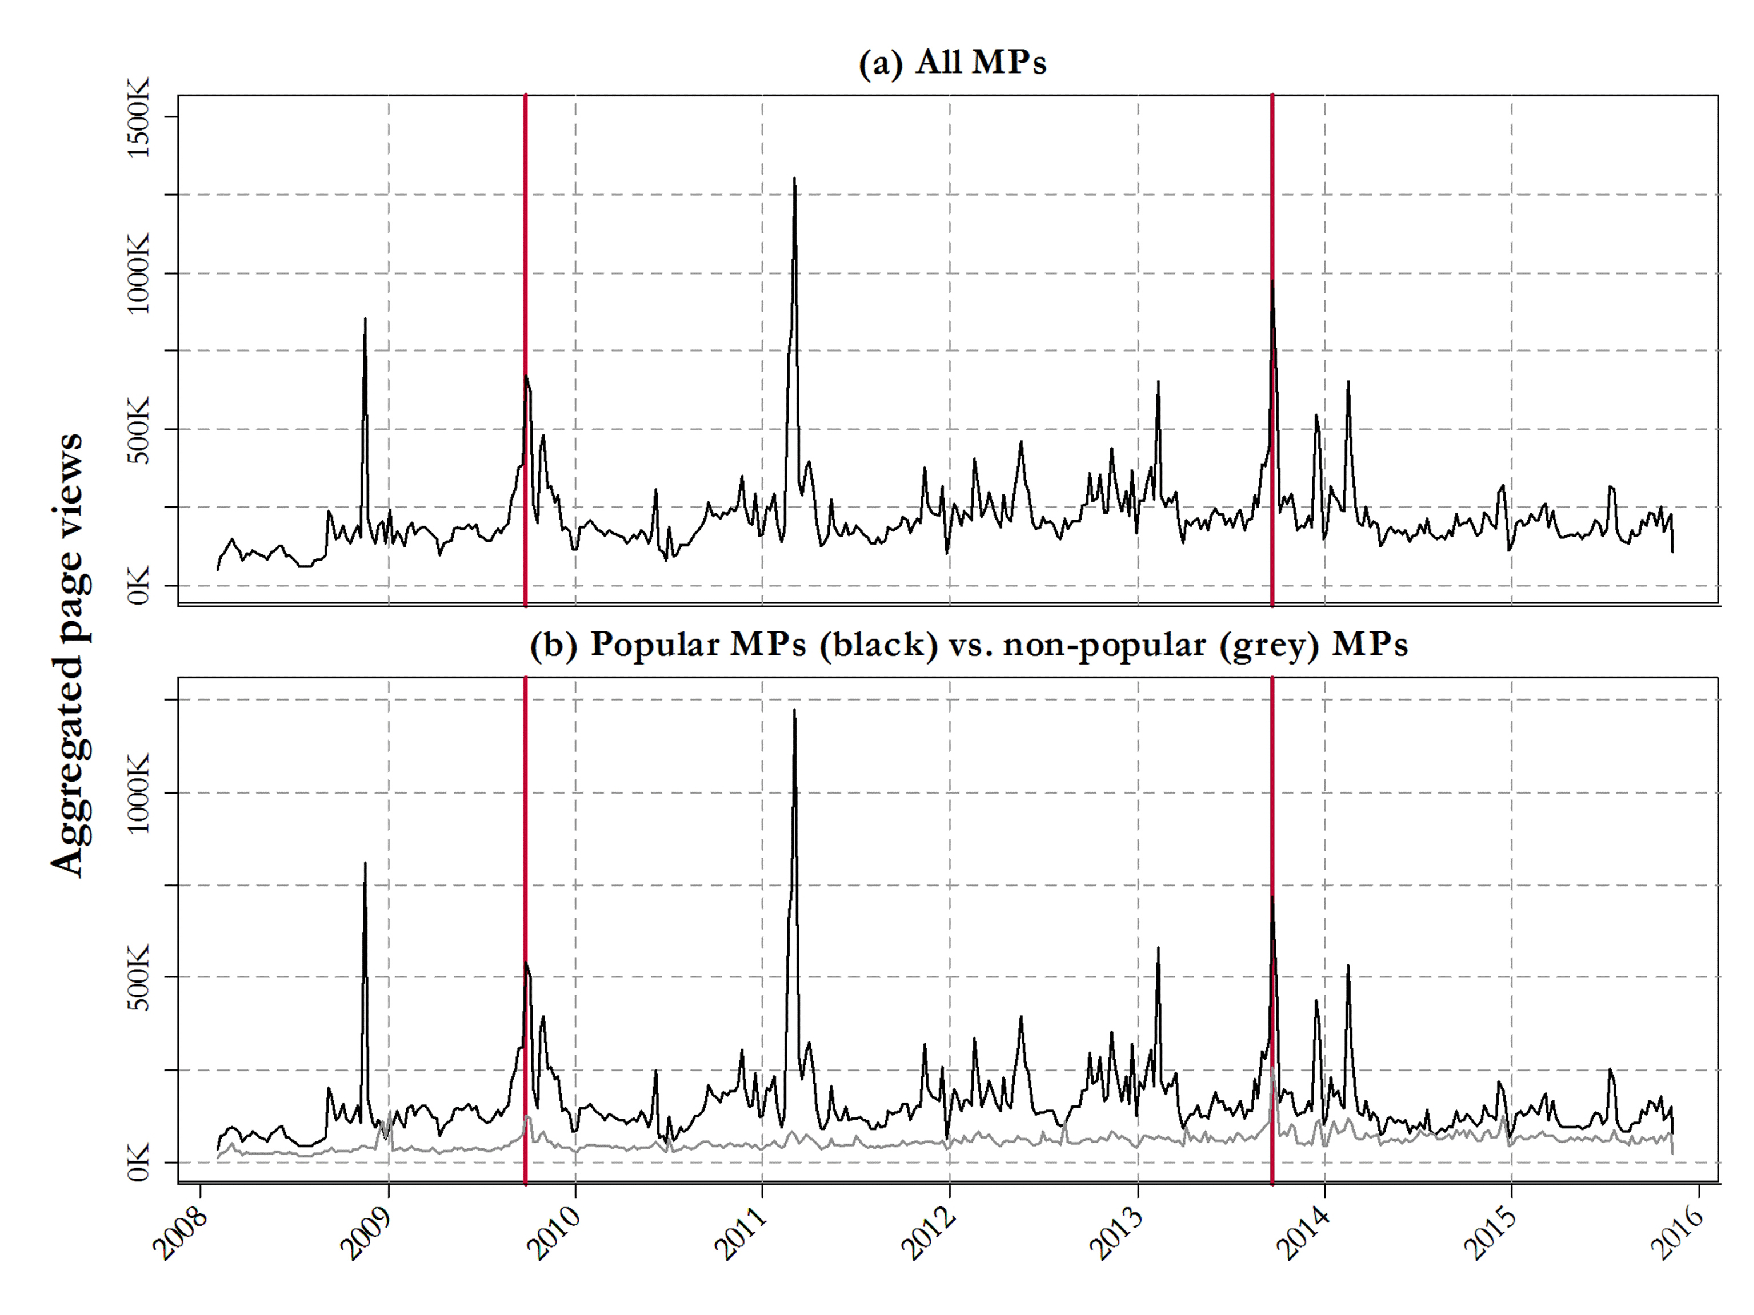
\includegraphics[scale=.33]{figure1.pdf}
	\vspace{-.5cm}
	\caption{Page views of German MPs’ Wikipedia entries.}
	% MAYBE ADD USA HOUSE TRAFFIC
\end{center}
\end{figure}
\end{frame}

\begin{frame}{Motivation}
\begin{figure}[t]
\begin{center}
\vspace{-.1cm}
	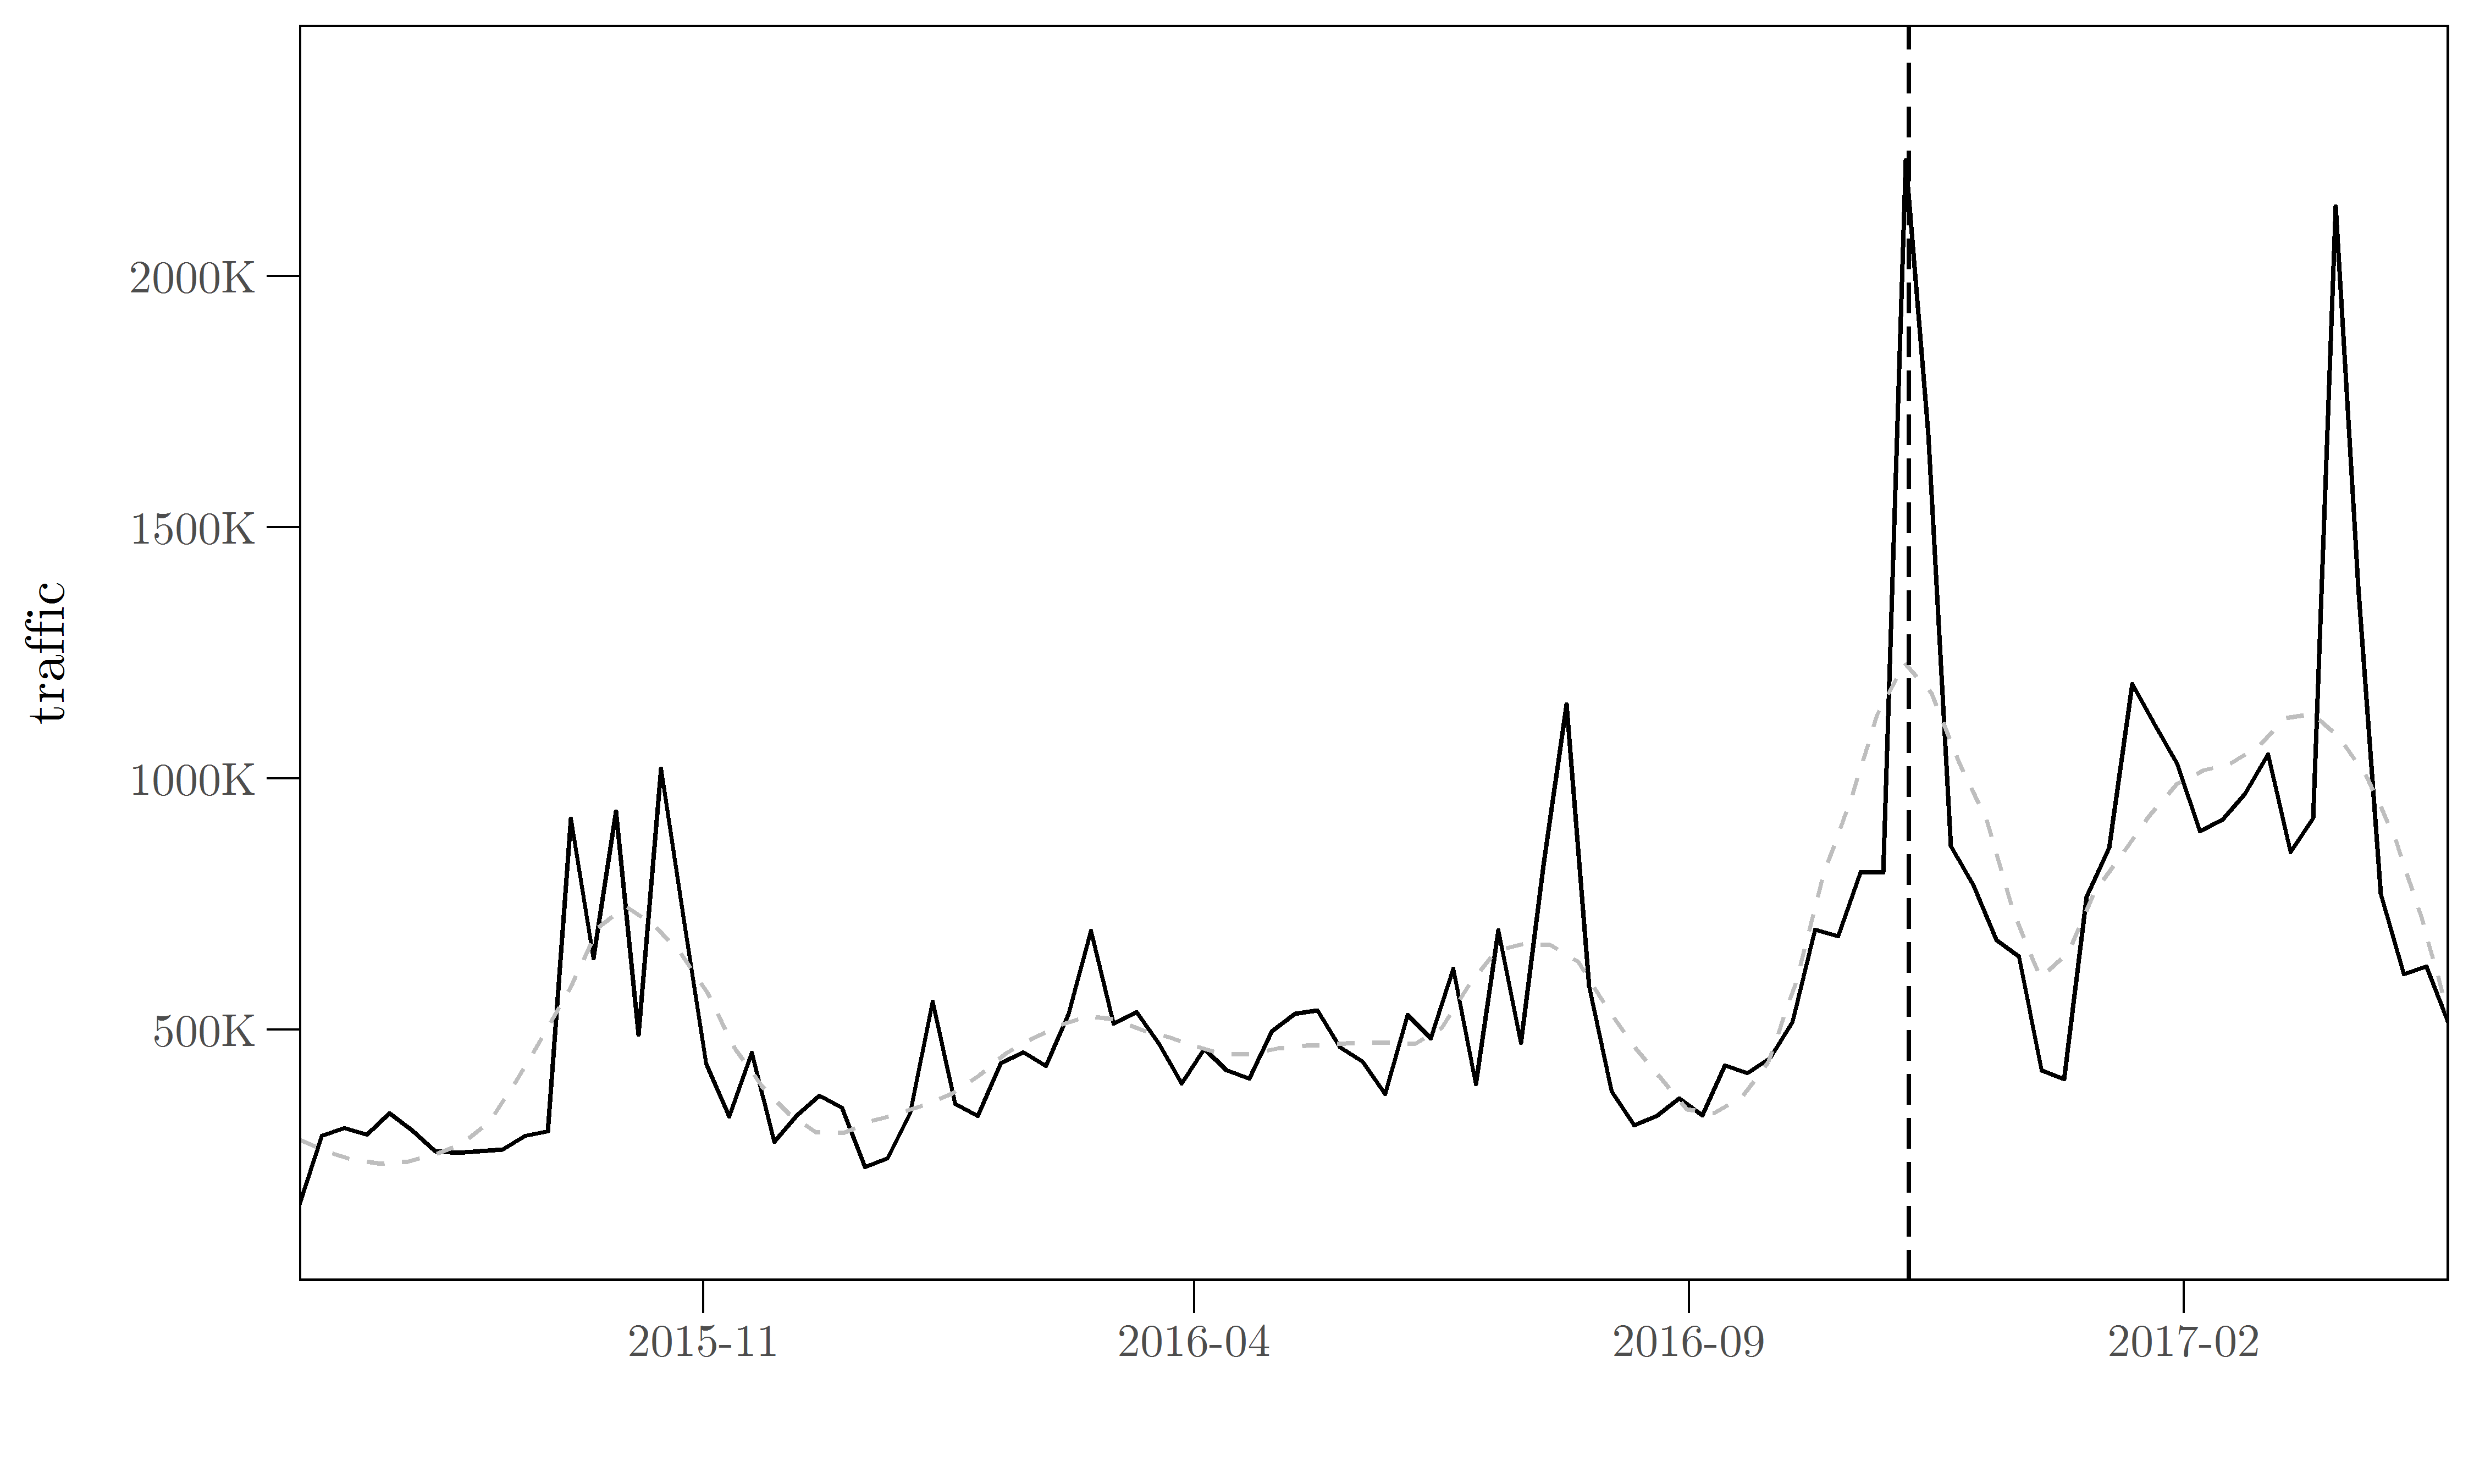
\includegraphics[scale=.53]{usah_time5.png}
	\vspace{-.5cm}
	\caption{Page views of US Representatives’ Wikipedia entries.}
	% MAYBE ADD USA HOUSE TRAFFIC
\end{center}
\end{figure}
\end{frame}

\begin{frame}{Motivation}
\begin{columns}
  \column{.65\textwidth}
  \begin{block}{legislatoR}
\begin{itemize}
	\item Resource \textbf{efficient}: one stop shop for broad and deep data
	\item Easily \textbf{accessible} from R with simple function calls
	\item Facilitates data \textbf{integration} and \textbf{replication} efforts
	\item It's \textbf{free}!
\end{itemize}
\end{block}     
 \column{.3\textwidth}
 \vspace{.2cm}

\includegraphics[width=\textwidth]{logo.png}
\end{columns}
\end{frame}

\section{Content and Structure}
\begin{frame}{Content and data structure}
\begin{block}{Content}
\begin{itemize}
	\item Currently \textbf{32,533 elected politicians}, all sessions of parliamentary chambers of Austria, Canada, the Czech Republic, France, Germany, Ireland, Scotland, UK, and the US (House and Senate)
	\pause
	\item \textbf{nine datasets} for each legislature:
	\item[] \begin{itemize}
			  \item[1.] \textit{Core} (basic sociodemographic data)
			  \item[2.] \textit{Political} (basic political data)	  
			  \item[3.] \textit{History} (full revision records of Wikipedia biographies)
			  \item[4.] \textit{Traffic} (daily user traffic on Wikipedia biographies)
			  \item[5.] \textit{Social} (social media handles and personal website URLs)
			  \item[6.] \textit{Portrait} (URLs to Wikipedia portraits, facial recognition estimates)
			  \item[7.] \textit{Office} (public offices)
			  \item[8.] \textit{Profession} (professions)
			  \item[9.] \textit{IDs} (identifiers linking to another file, database, or website)
		\end{itemize}
\end{itemize}
\end{block}
\end{frame}

\begin{frame}{Content and data structure}
\begin{figure}[t]
\begin{center}
\vspace{-.3cm}
	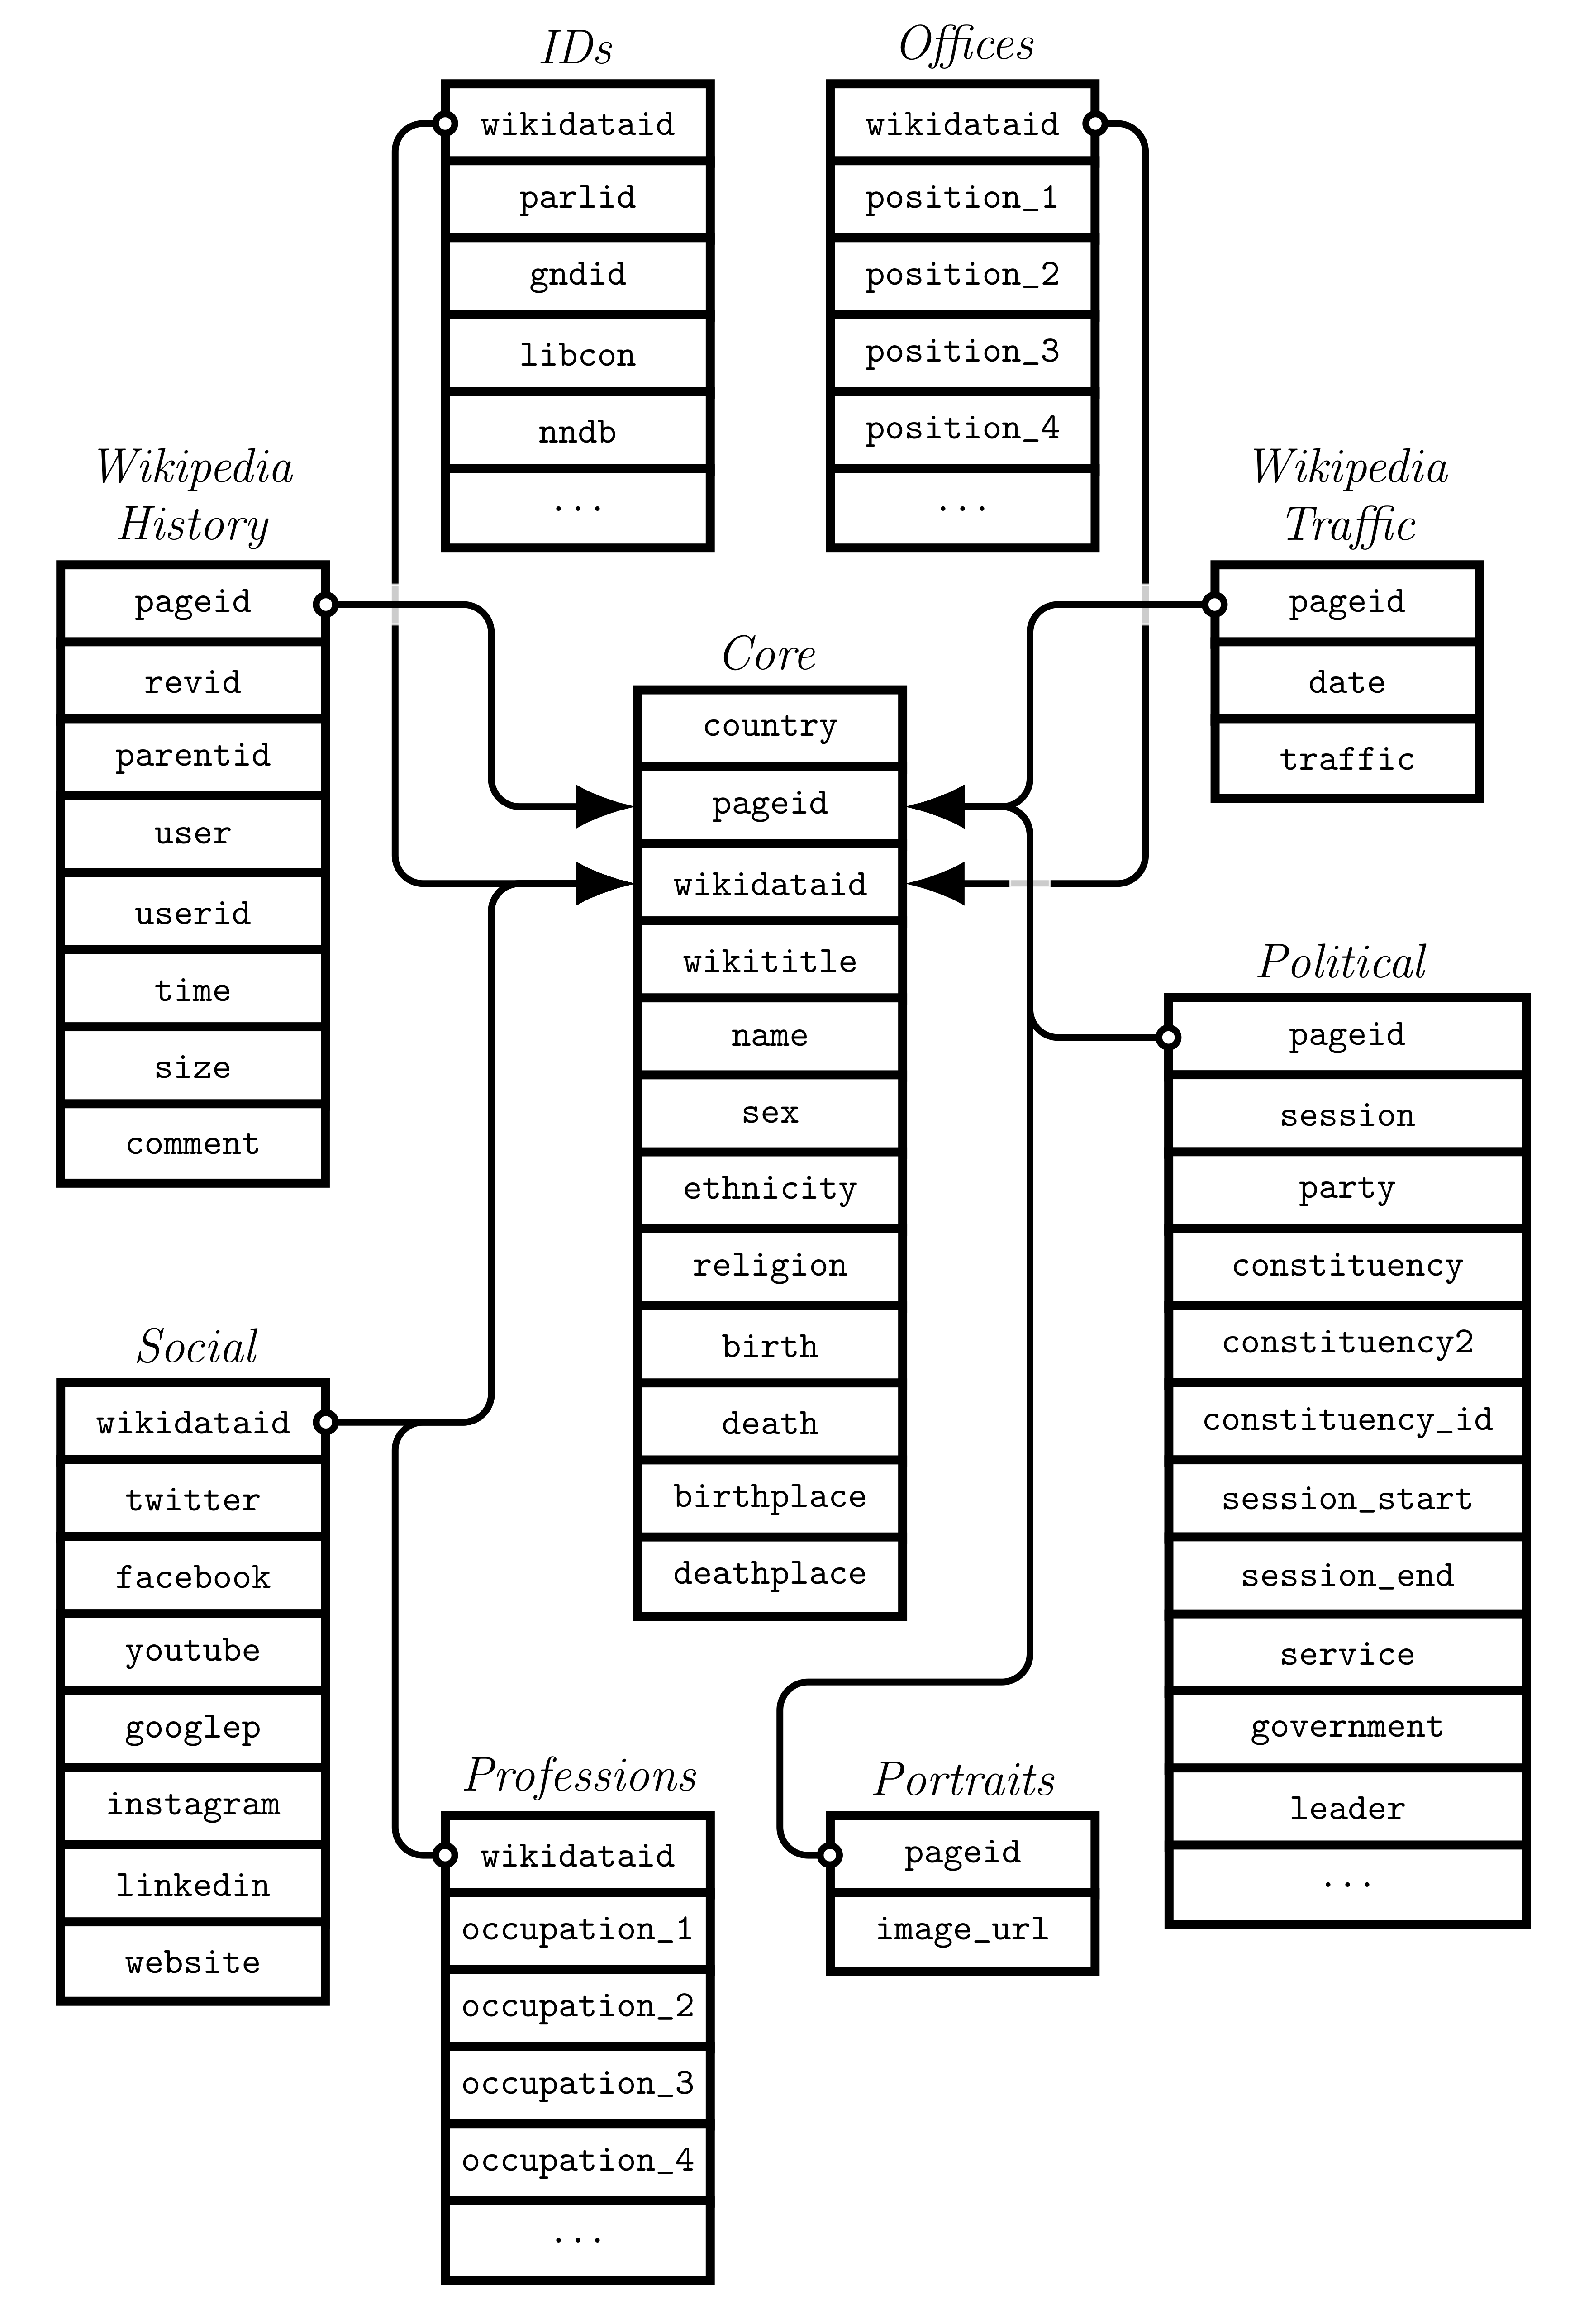
\includegraphics[height=.85\textheight]{data-structure.png}
\end{center}
\end{figure}
\end{frame}

\begin{frame}{Content and data structure}
\begin{block}{Structure}
\begin{itemize}
	\item \textbf{relational} Individual-level data -- all datasets joinable with \textit{Core} dataset via two keys  (Wikipedia page or Wikidata ID)
\end{itemize}
\end{block}
\pause
\begin{block}{Sources}
\begin{itemize}
	\item \textbf{Automated} data extraction (XPath, Web APIs)
	\item Face++ Cognitive Services API, Wikimedia Commons, Wikidata API, Wikipedia, Wikipedia API
\end{itemize}
\end{block}
\pause
\begin{block}{Issues}
\begin{itemize}
	\item Dependence on data coverage of sources, collaborative effort (but that's a feature, not a bug!)
	\item In part substantial amount of missings
\end{itemize}
\end{block}
\end{frame}

\section{Usage}


\begin{frame}{Usage}
\begin{block}{Installation}
\scriptsize{\texttt{> \# install from GitHub}} \\
\scriptsize{\texttt{> devtools::install\char`_github("saschagobel/legislatoR")}} \\
\scriptsize{\texttt{> \# load and attach}} \\
\scriptsize{\texttt{> library(legislatoR)}}
\end{block}
\vspace{1cm}
\pause
\Large \centering For up-to-date information, check out \\ \url{https://github.com/saschagobel/legislatoR}
\end{frame}

\iffalse
\begin{frame}{Usage}
\begin{block}{Installation (not on CRAN yet!)}
\scriptsize{\texttt{> \# install from GitHub}} \\
\scriptsize{\texttt{> devtools::install\char`_github("saschagobel/legislatoR")}} \\
\scriptsize{\texttt{> \# load and attach}} \\
\scriptsize{\texttt{> library(legislatoR)}}
\end{block}
\pause
\begin{block}{Get data}
\begin{itemize}
\item \texttt{get\char`_\{dataset\}()} fetches data from repository
\item function takes one argument: \texttt{legislature}
\item legislature codes: \texttt{austria}, \texttt{france}, \texttt{germany}, \texttt{ireland}, \texttt{usah}, \texttt{usas} 
\end{itemize}
\scriptsize{\texttt{> \# assign Core dataset for US House of Representatives into environment}} \\
\scriptsize{\texttt{> congressmen <- get\char`_core(legislature = "usah")}}
\end{block}
\end{frame}

\begin{frame}{Usage}
\begin{block}{Join and subset data}
\begin{itemize}
\item data can be joined and subsetted while being fetched
\item memory only allocated by parts assigned into environment
\end{itemize}
\scriptsize{\texttt{> \# assign Core dataset for US House of Representatives from 115th}}\\ 
\scriptsize{\texttt{> \# session into environment}} \\
\scriptsize{\texttt{> congressmen115 <- semi\char`_join(x = get\char`_core(legislature = "usah"),}}\\
\scriptsize{\texttt{\enspace\enspace\enspace\enspace\enspace\enspace\enspace\enspace\enspace\enspace\enspace\enspace\enspace\enspace\enspace\enspace\enspace\enspace\enspace\enspace\enspace\enspace\enspace\enspace\enspace\enspace\enspace\enspace\enspace\enspace y = filter(get\char`_political(legislature =}} \\
\scriptsize{\texttt{\enspace\enspace\enspace\enspace\enspace\enspace\enspace\enspace\enspace\enspace\enspace\enspace\enspace\enspace\enspace\enspace\enspace\enspace\enspace\enspace\enspace\enspace\enspace\enspace\enspace\enspace\enspace\enspace\enspace\enspace\enspace\enspace\enspace\enspace "usah"), session == 115),}}\\
\scriptsize{\texttt{\enspace\enspace\enspace\enspace\enspace\enspace\enspace\enspace\enspace\enspace\enspace\enspace\enspace\enspace\enspace\enspace\enspace\enspace\enspace\enspace\enspace\enspace\enspace\enspace\enspace\enspace\enspace\enspace\enspace\enspace by = "pageid")}}\\
\scriptsize{\texttt{> \# append Wikipedia revision to congressmen115}}\\ 
\scriptsize{\texttt{> congressmen115h <- left\char`_join(x = congressmen115,}}\\
\scriptsize{\texttt{\enspace\enspace\enspace\enspace\enspace\enspace\enspace\enspace\enspace\enspace\enspace\enspace\enspace\enspace\enspace\enspace\enspace\enspace\enspace\enspace\enspace\enspace\enspace\enspace\enspace\enspace\enspace\enspace\enspace\enspace\enspace y = get\char`_history(legislature = "usah"),}}\\ 
\scriptsize{\texttt{\enspace\enspace\enspace\enspace\enspace\enspace\enspace\enspace\enspace\enspace\enspace\enspace\enspace\enspace\enspace\enspace\enspace\enspace\enspace\enspace\enspace\enspace\enspace\enspace\enspace\enspace\enspace\enspace\enspace\enspace\enspace by = "pageid")}}
\end{block}
\pause
\begin{block}{Get help}
\scriptsize{\texttt{> \# call legislatoR help file for an overview of function calls}}\\
\scriptsize{\texttt{> ?legislatoR}}\\
\scriptsize{\texttt{> \# call help file for 'History' dataset}}\\
\scriptsize{\texttt{> ?get\char`_history}}\\
\end{block}
\end{frame}

\section{Use Cases}
\begin{frame}{Use Cases (1)}
\begin{itemize}
\item Political advertising on the Wikipedia marketplace of information (Göbel and Munzert Forthcoming)
\end{itemize}
\begin{block}{Existing research}
\begin{itemize}
	\item capitalizes on free accessibility and editability
	\item political content negotiated	(Neff et al. 2013)
	\item politically biased editing (Kalla and Aronow 2015)
\end{itemize}
\end{block}
\pause
\begin{block}{Research question and contribution}
\begin{itemize}
	\item \textbf{if}, \textbf{how}, and \textbf{why} politicians take part in political interaction on Wikipedia?
	\item study elite behavioral patterns via Wikipedia
	\item role of the platform for professionalization of campaigning
\end{itemize}
\end{block}
\end{frame}

\begin{frame}{Use Cases (1)}
$\bullet$ Wikipedia biographies constitute highly efficient tool for electoral campaigning and political marketing
\begin{table}[h]
  \centering
  \small
    \begin{tabularx}{\linewidth}{XXX}
    \hline
    connect & sway & control  \\
    \hline
    increase online & advertise, claim & shape information, \\
    visibility, target & credit, take & bypass \\ 
    voters & position & media/party filter, \\
    & & remain undetected \\
    \hline
    \end{tabularx}
%
\end{table}
\pause
\begin{block}{Expectations}
Usage and scope differ by incentive to cultivate a personal vote, temporal context, age, party affiliation, popularity, geographical location
%
\end{block}
\end{frame}



\begin{frame}{Use Cases (1)}
\begin{block}{Empirical strategy}
\begin{itemize}
	\item explore edit histories of Wikipedia biographies
%
	\item trace edits originating from parliament's IP range
%
	\item explain edit patterns with strategic incentives and sociodemographics
\end{itemize}
\end{block}
\pause
\begin{block}{Data}
\begin{itemize}
	\item outcome: count of edits per biography
%
	\item predictors: political and sociodemographic MP characteristics and page metrics
%
	\item source: scraping of Wikipedia and MPs' Bundestag page HTMLs using XPath and regexp
\end{itemize}
\end{block}
\end{frame}

\begin{frame}{Use Cases (1)}
\begin{block}{Case}
\begin{itemize}
	\item German MPs; 2005-2015; 1,100 MPs; 108,775 edits
% 
	\item third largest Wikipedia, second largest number of edits
% 
	\item exploit mixed electoral system (district vs. list candidates)
% 
\end{itemize}
\end{block}
\pause
\begin{block}{Limitations}
\begin{itemize}
	\item edits cannot be linked to MPs directly
% 
	\item MPs `true' editing activity possibly underreported
% 
	\item actual purpose of edits not revealed by aggregate data
% 
\end{itemize}
\end{block}
\end{frame}

\begin{frame}{Use Cases (1)}
\begin{block}{Results}
\begin{itemize}
	\item \textbf{substantive public interest} in MPs' Wikipedia entries
	\item qualitative \textbf{evidence} for various kinds \textbf{of marketing}
	\item \textbf{51 percent} of the sampled \textbf{MP}s exhibit \textbf{edits} from the parliament's IP range
	\item \textbf{2.2 percent} (\textbf{$\approx$ 2400}) \textbf{of all edits} can be traced back to the German Bundestag
	\item \textbf{no increase}d activity visible \textbf{before elections}
	\item predictors highlight \textbf{strategic incentives}
\end{itemize}
\end{block}
\end{frame}

\begin{frame}{Use Cases (1)}
\vspace{0.2cm}
Typology of edits from parliament's IT network
\vspace{-0.2cm}
\small
\begin{table}
\begin{tabularx}{\linewidth}{lXX}
  \toprule
& category & example  \\ 
 \midrule
1. & non-substantial edits & correction of tense or typos \\
2. & private information sharing & information about childhood or housing shared \\
3. & CV shaping & information about life and career added/removed    \\
4. & provision of campaign information  & weblink to campaign page added \\
5. & highlighting of successes  & statements of electoral successes in comparison with competitors \\
6. & positive reframing  & `failures' framed as achievements \\
7. & removal of adverse information  & information about memberships or past life removed \\
  \bottomrule
\end{tabularx}
\end{table}
\end{frame}

\begin{frame}{Use Cases (1)}
\begin{figure}[t]
\begin{center}
\vspace{-.1cm}
	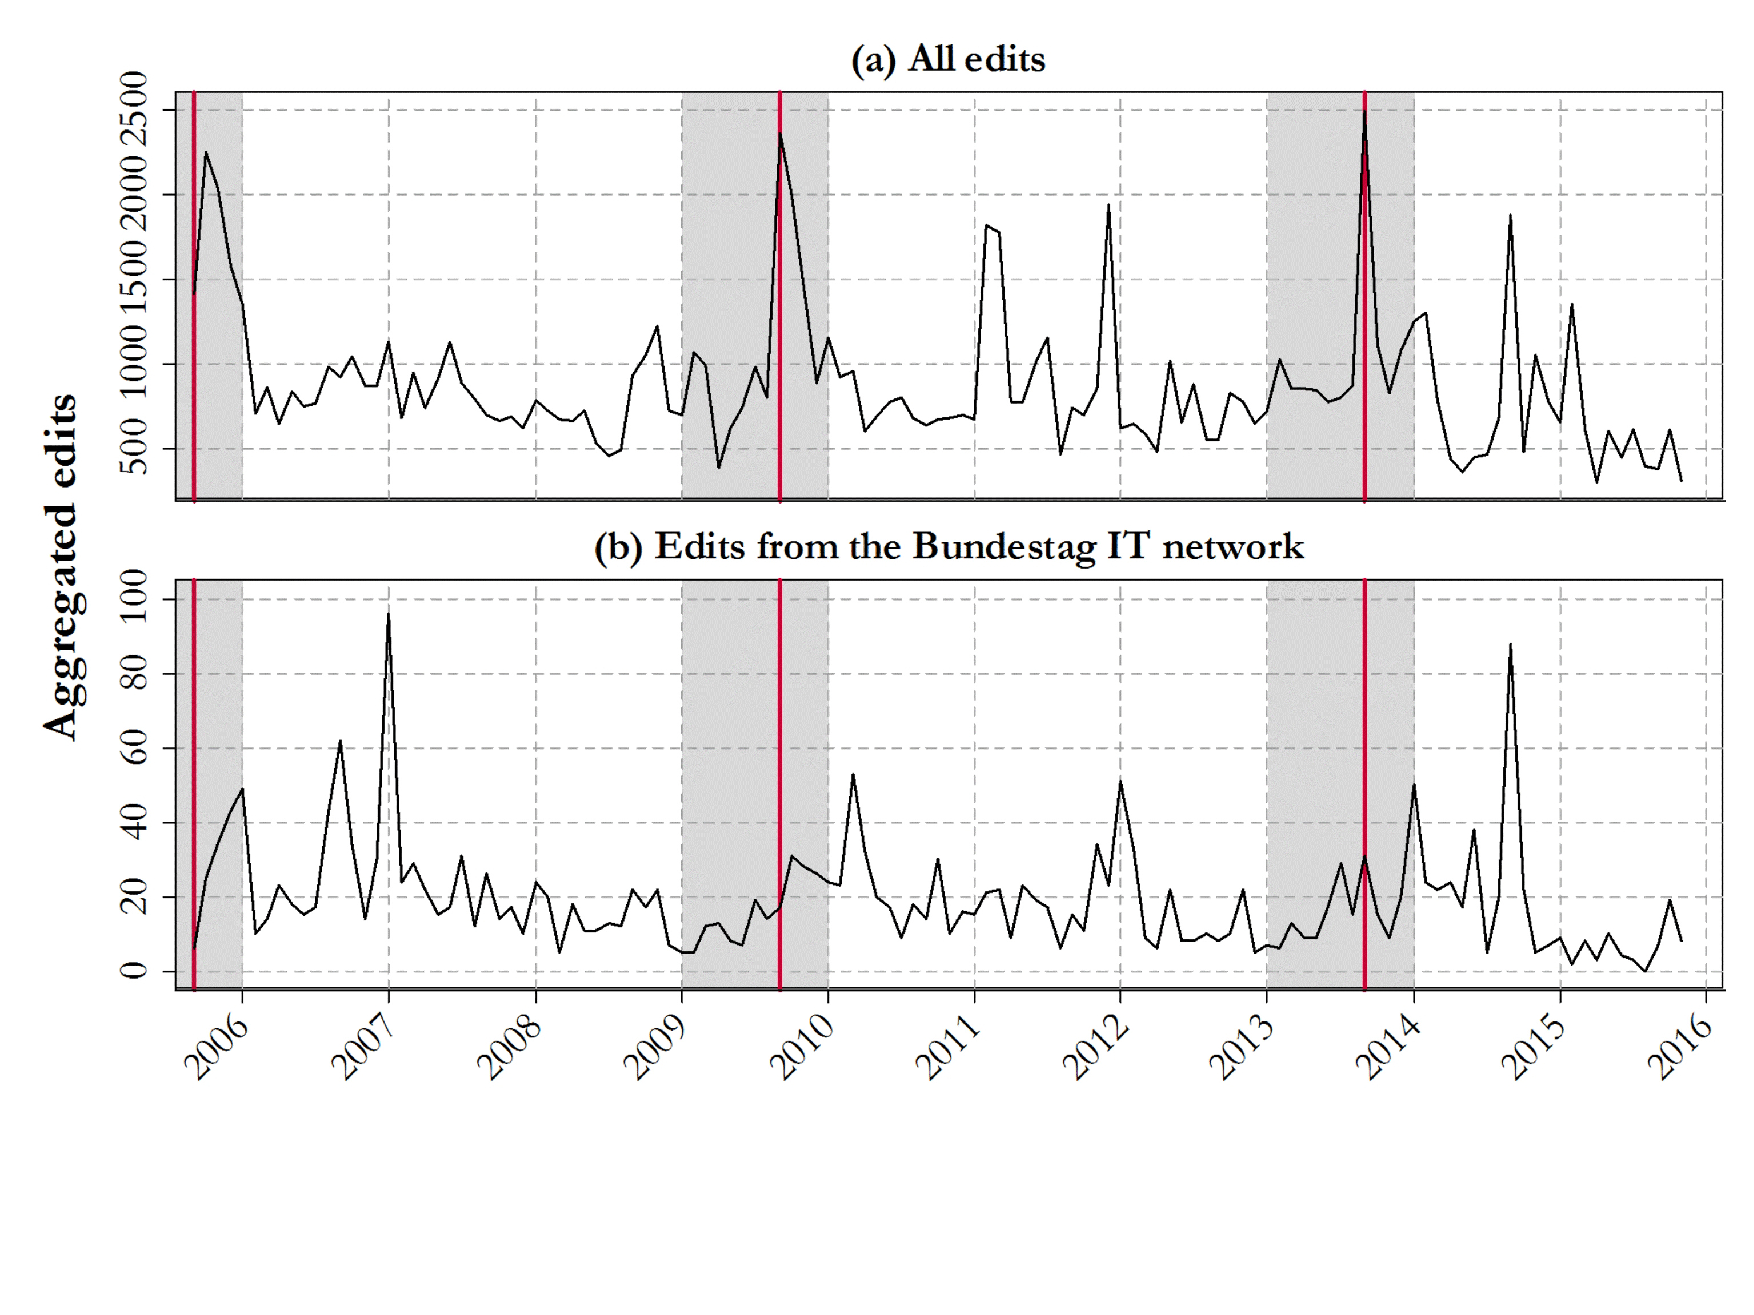
\includegraphics[scale=.36]{figure3.pdf}
	\vspace{-1.4cm}
	\caption{Edits on MPs' Wikipedia biographies over time.}
\end{center}
\end{figure}
\end{frame}

\begin{frame}{Use Cases (1)}
\vspace{0cm}
Estimates of factors driving edits from parliament's IP range
\vspace{-0.1cm}
\begin{figure}[t]
\begin{center}
	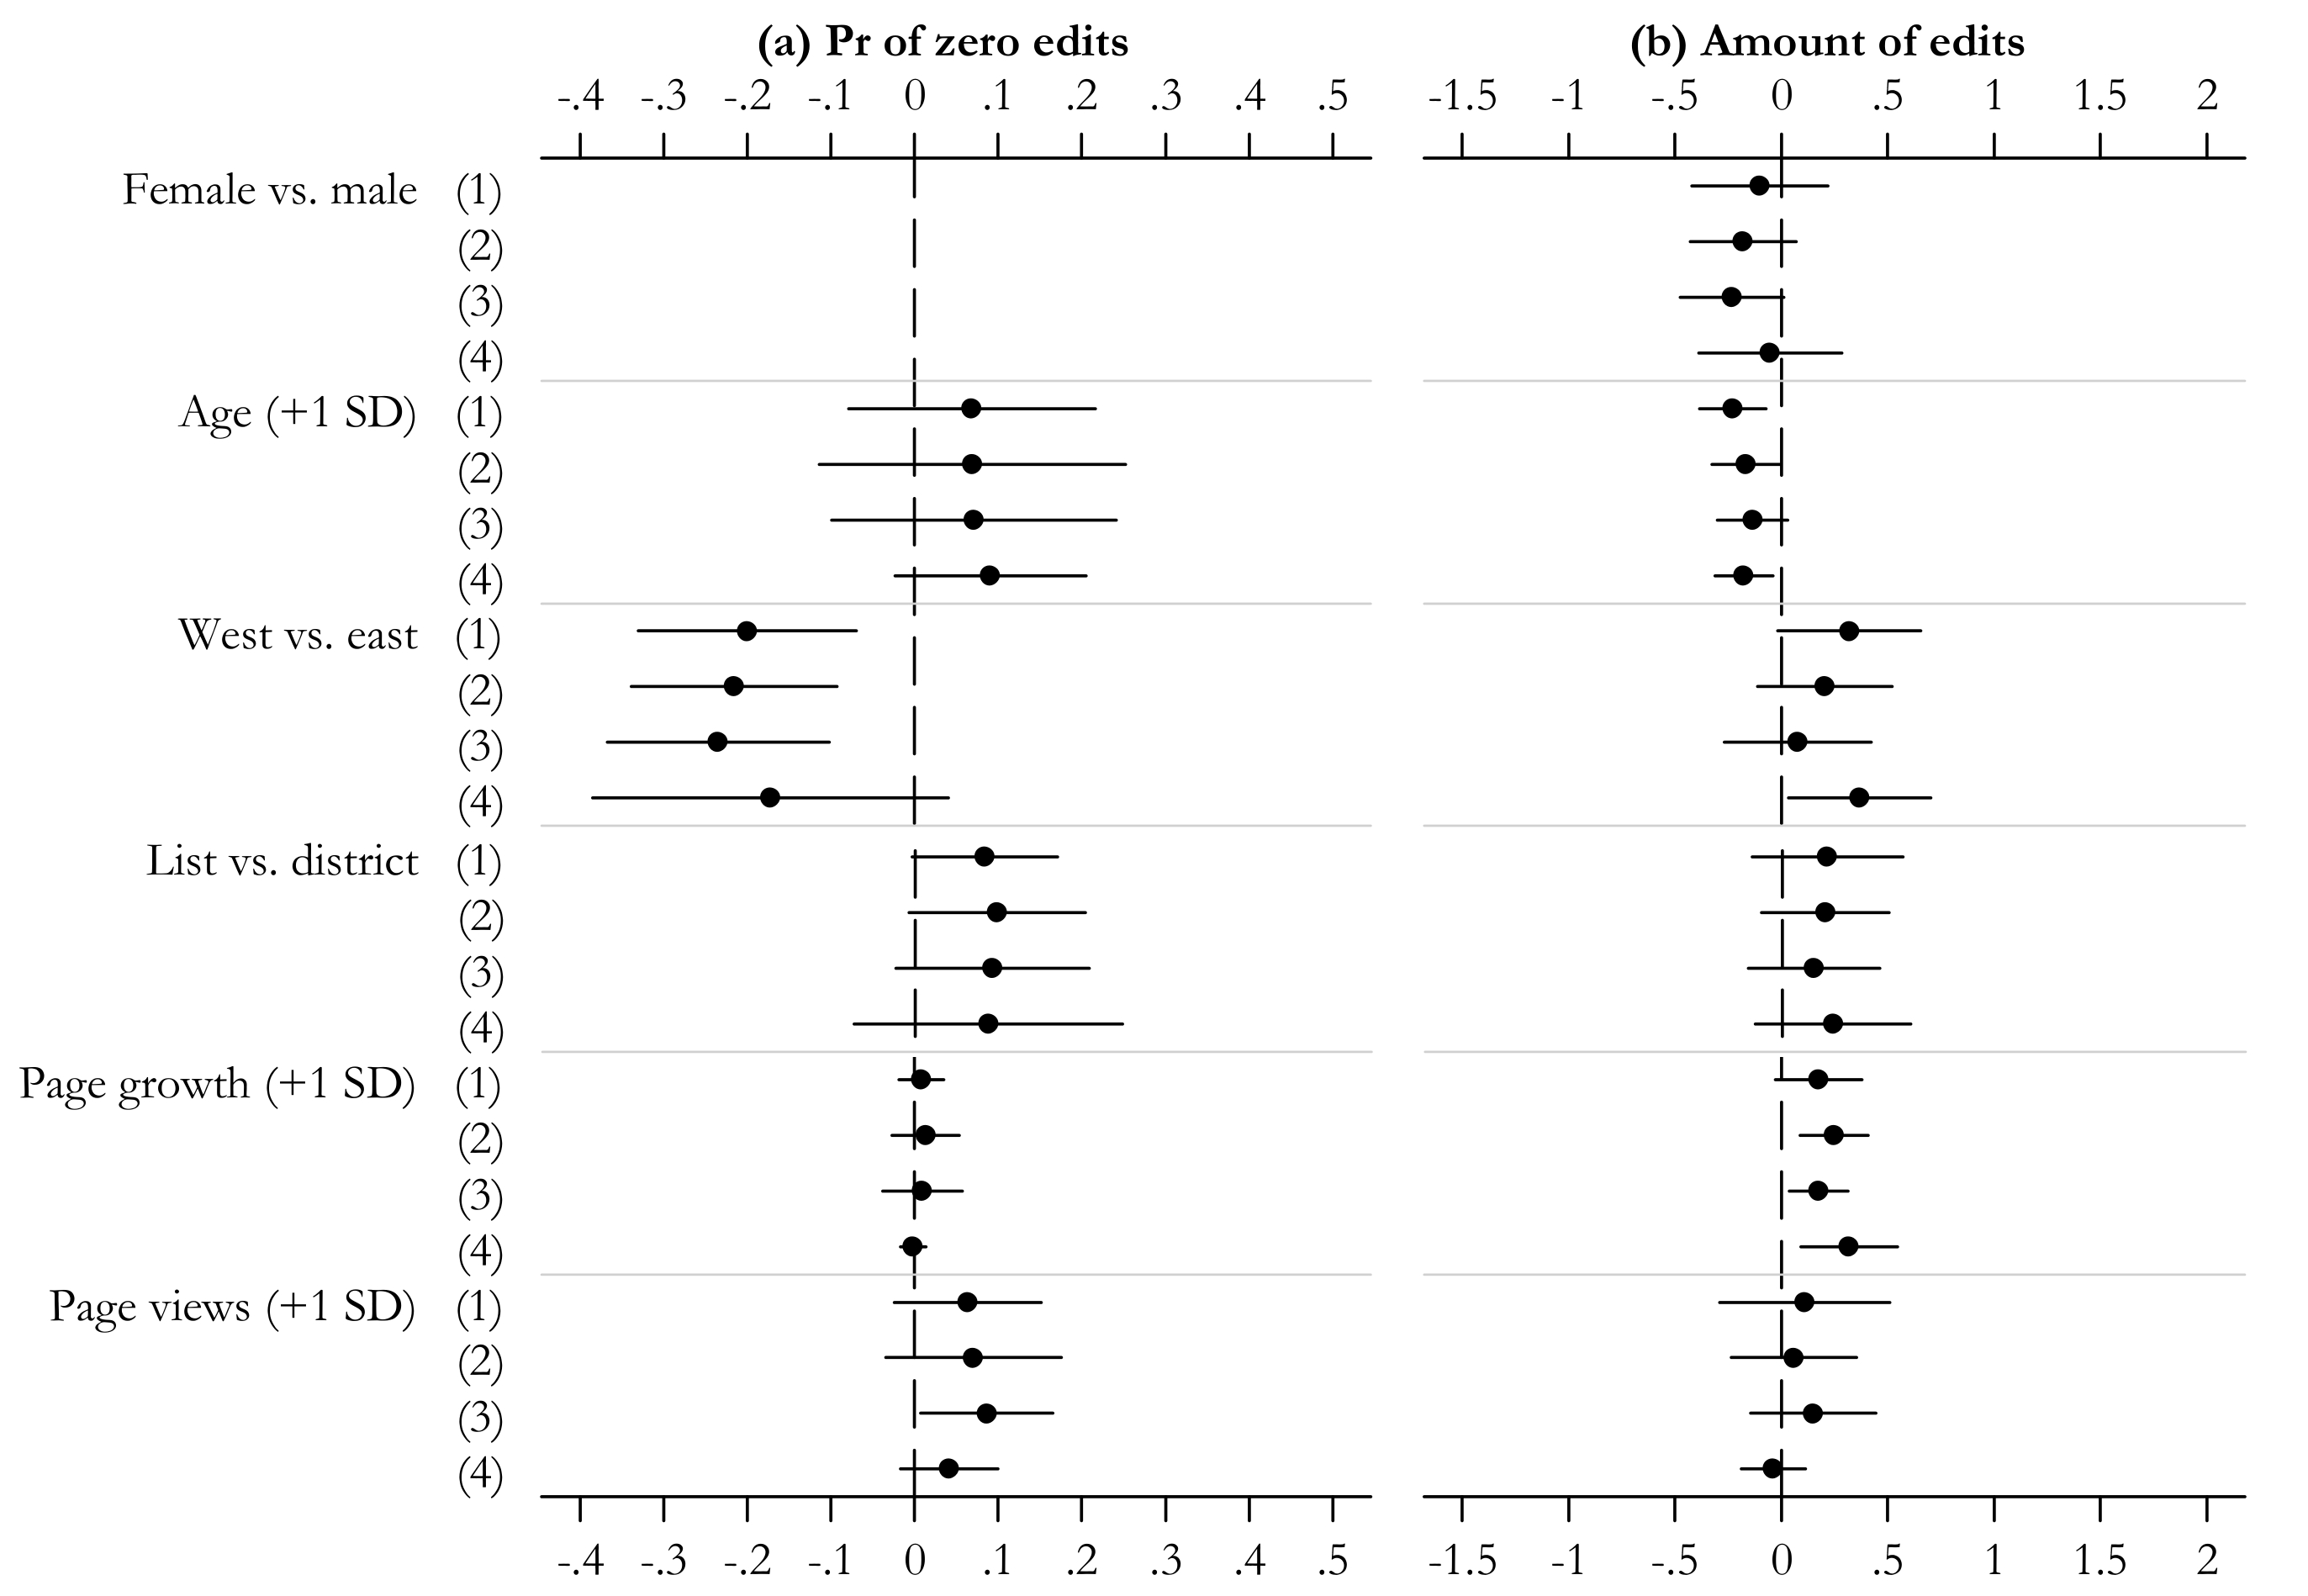
\includegraphics[scale=.75]{figure6.jpg}
		\vspace{-0.3cm}
	\caption{\tiny{Note: Based on ZINB models holding other predictors at observed values.}}
\end{center}
\end{figure}
\end{frame}

\begin{frame}{Use Cases (1)}
\begin{itemize}
\item 18th German Bundestag (continued)
\end{itemize}
\begin{figure}[t]
\begin{center}
\vspace{-.1cm}
	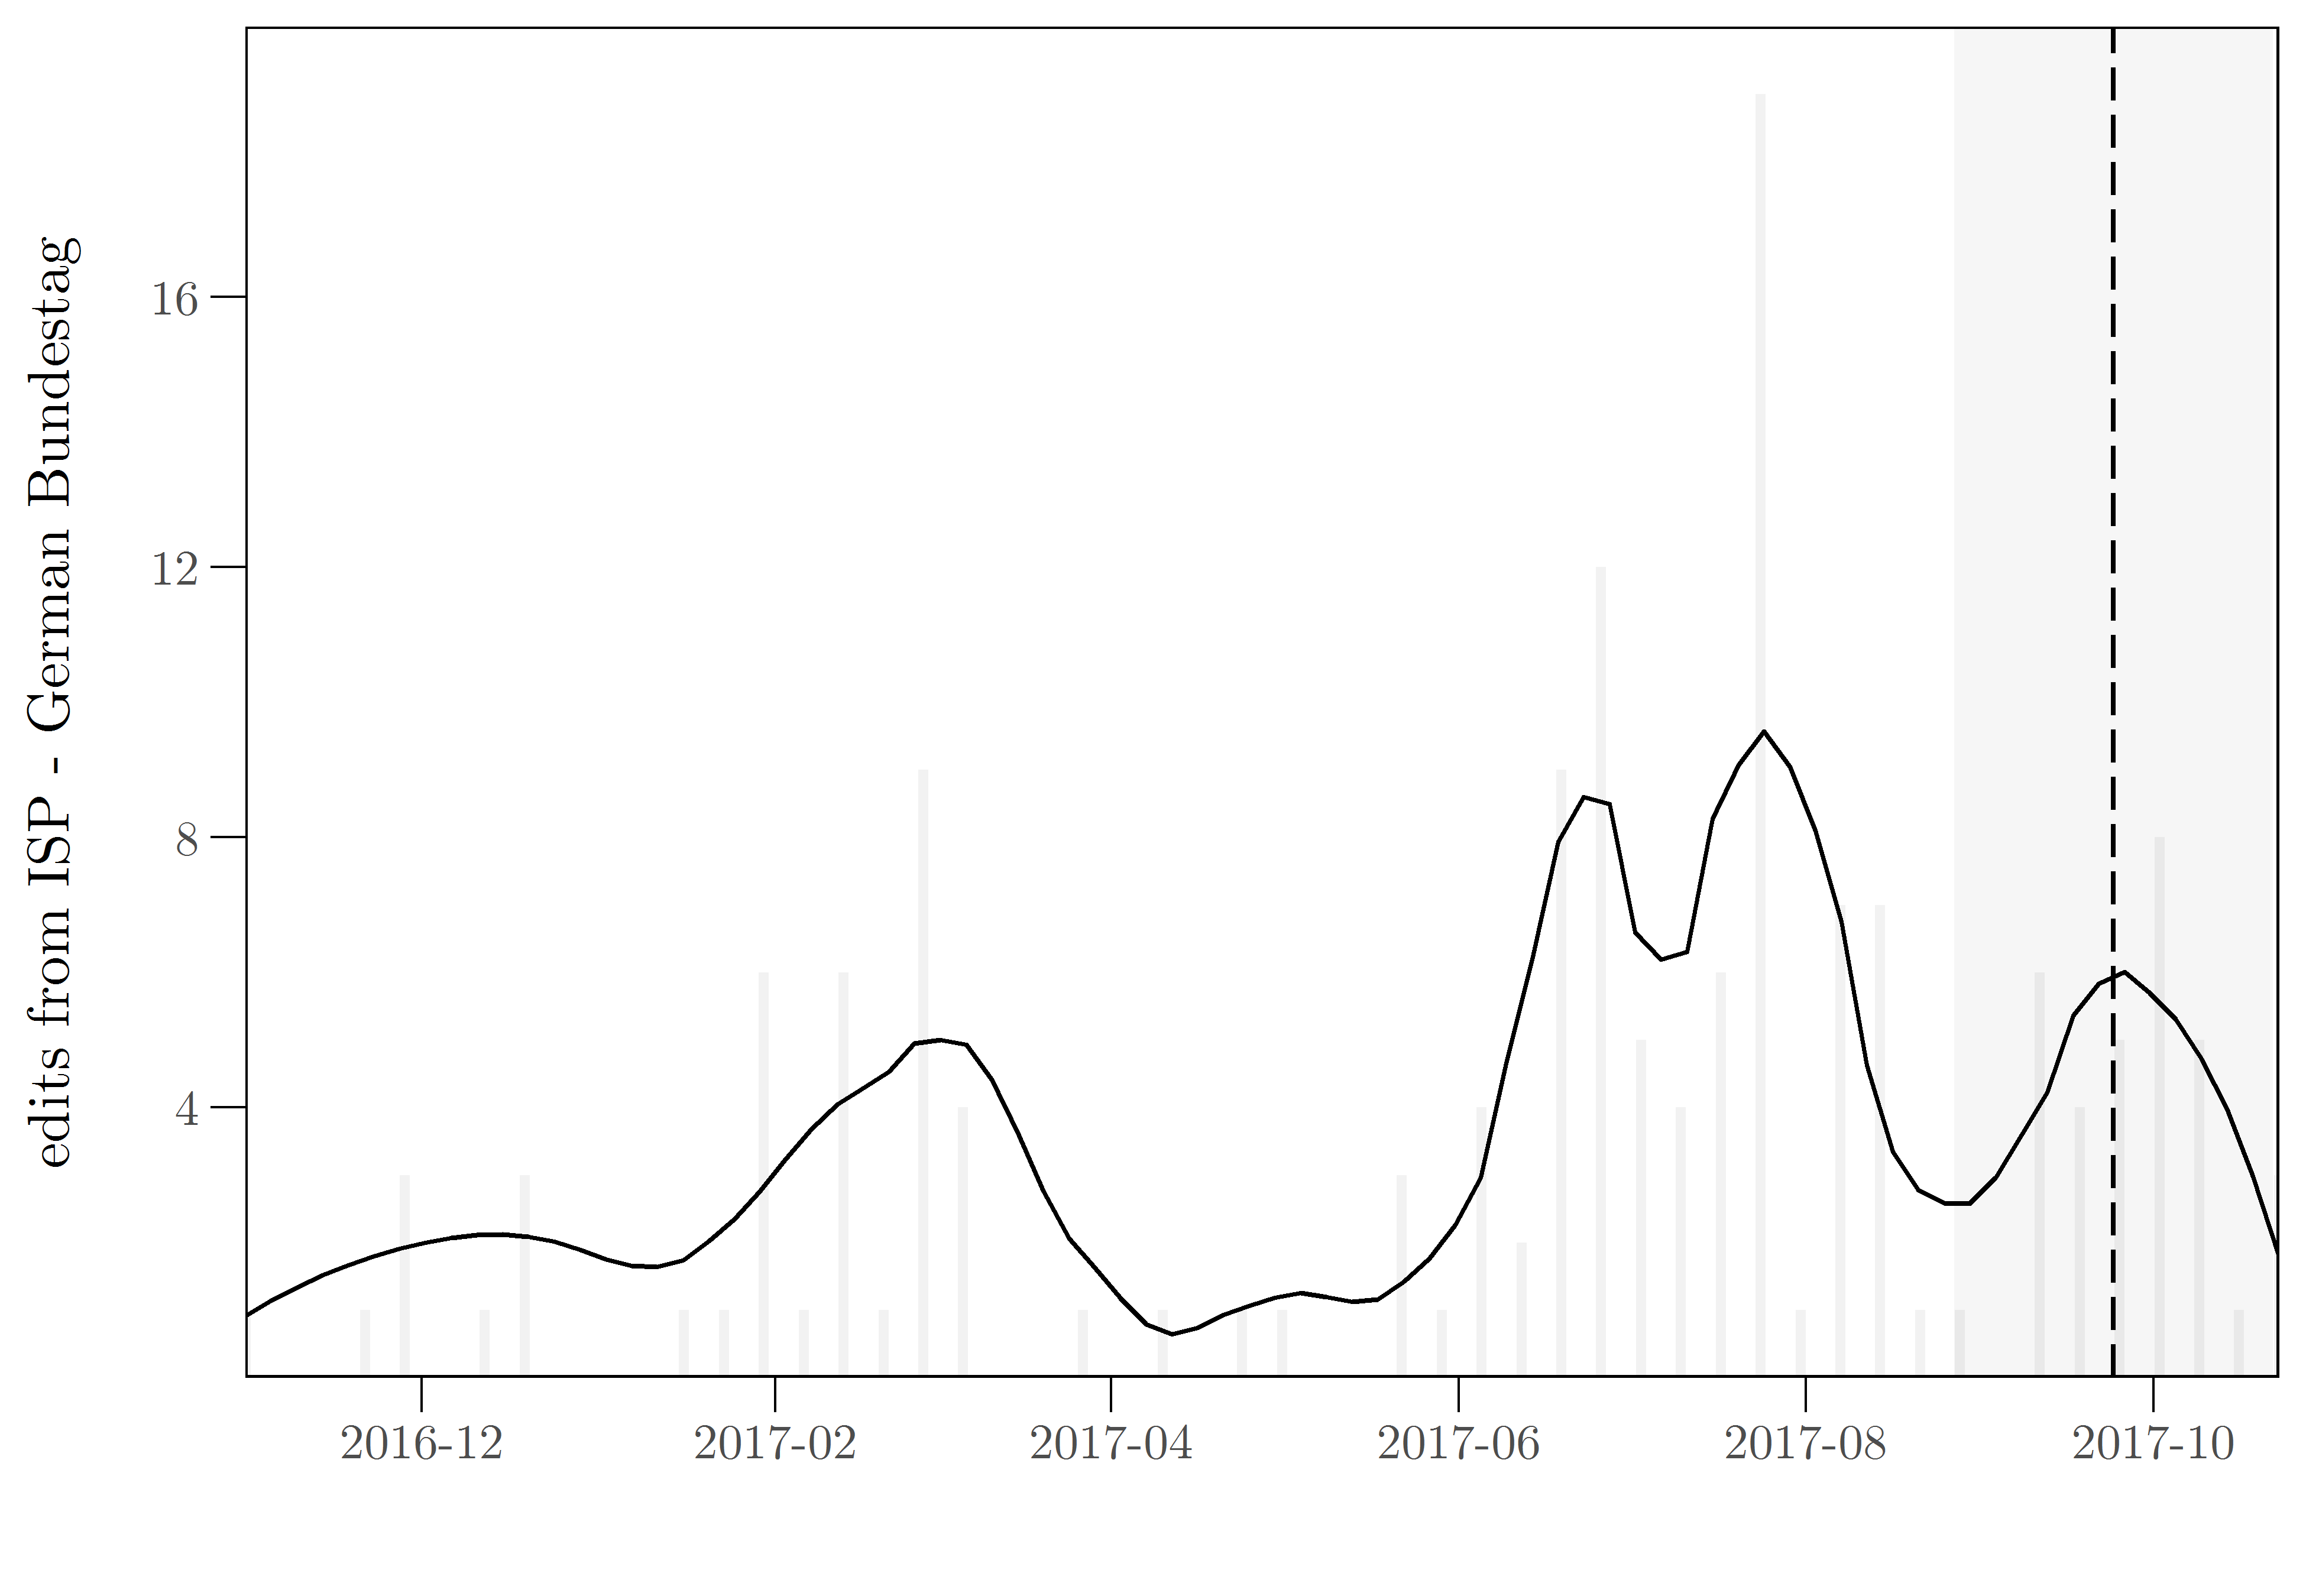
\includegraphics[scale=.63]{uc_1_germany_time.png}
	\vspace{-.5cm}
\end{center}
\end{figure}
\end{frame}

\begin{frame}{Use Cases (2)}
\begin{itemize}
\item 114th US House of Representatives
\end{itemize}
\begin{figure}[t]
\begin{center}
\vspace{-.1cm}
	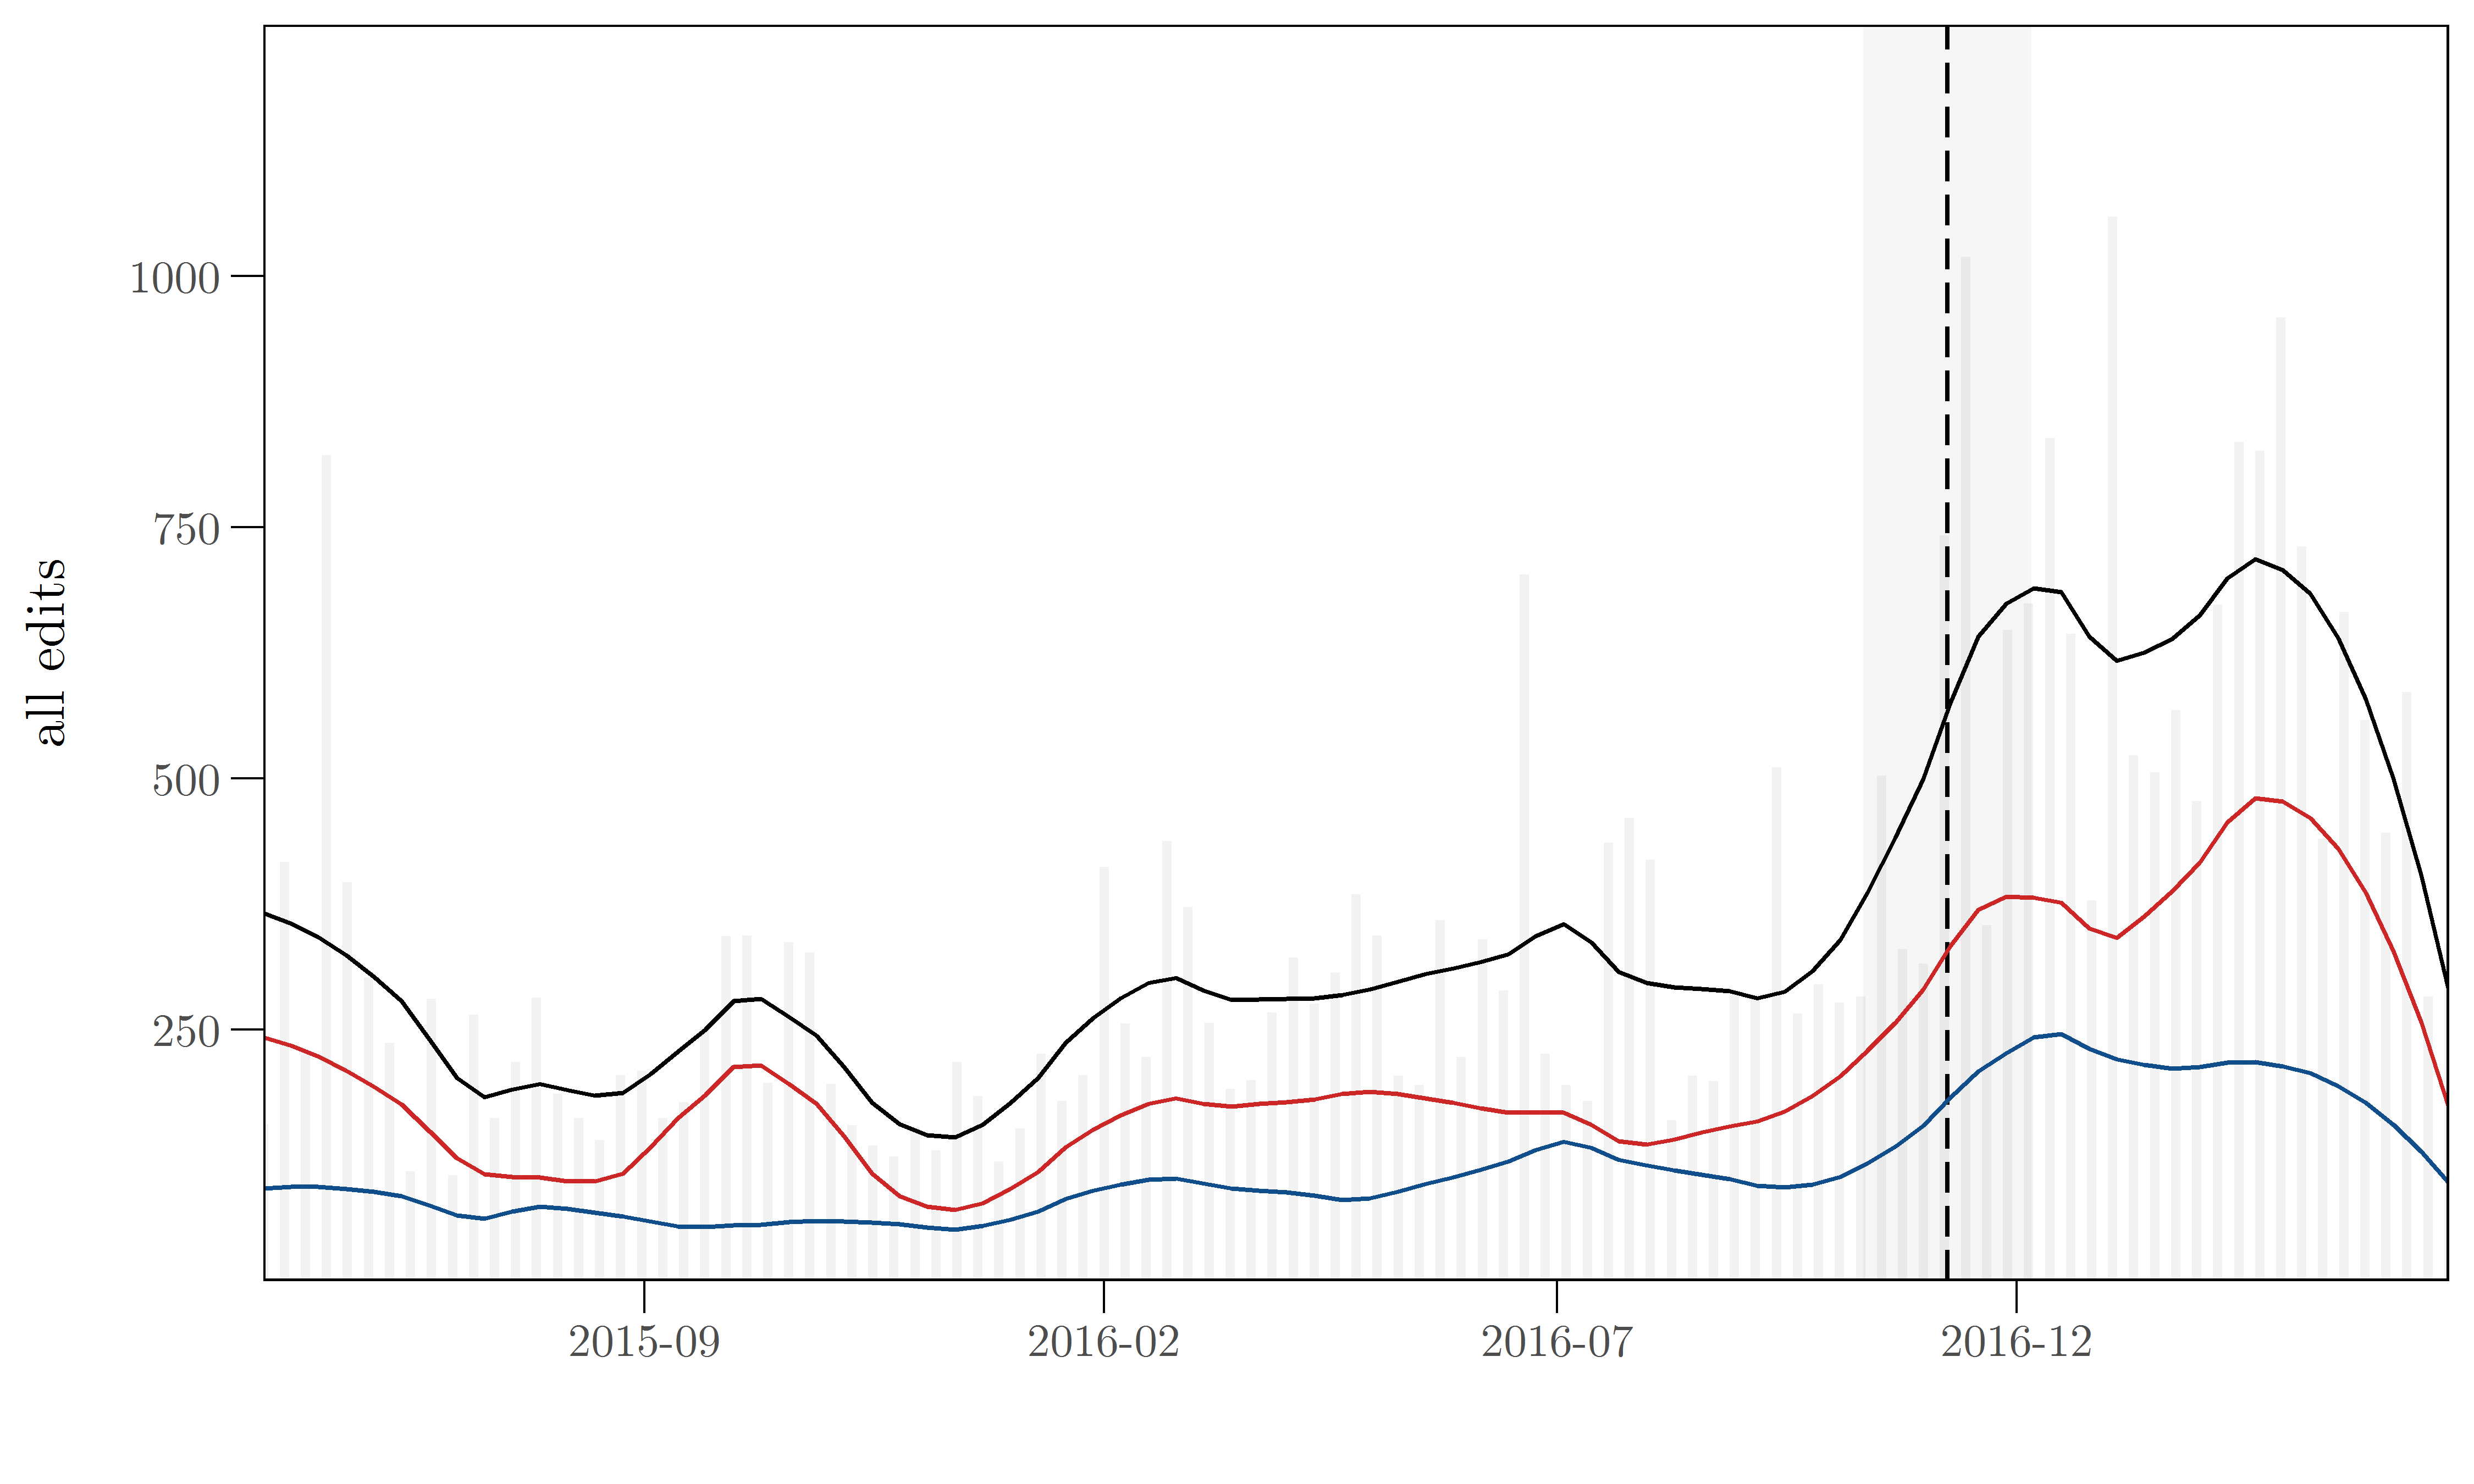
\includegraphics[scale=.55]{uc_2_usah_time1.png}
	\vspace{-.5cm}
\end{center}
\end{figure}
\end{frame}

\begin{frame}{Use Cases (2)}
\begin{figure}[t]
\begin{center}
\vspace{-.1cm}
	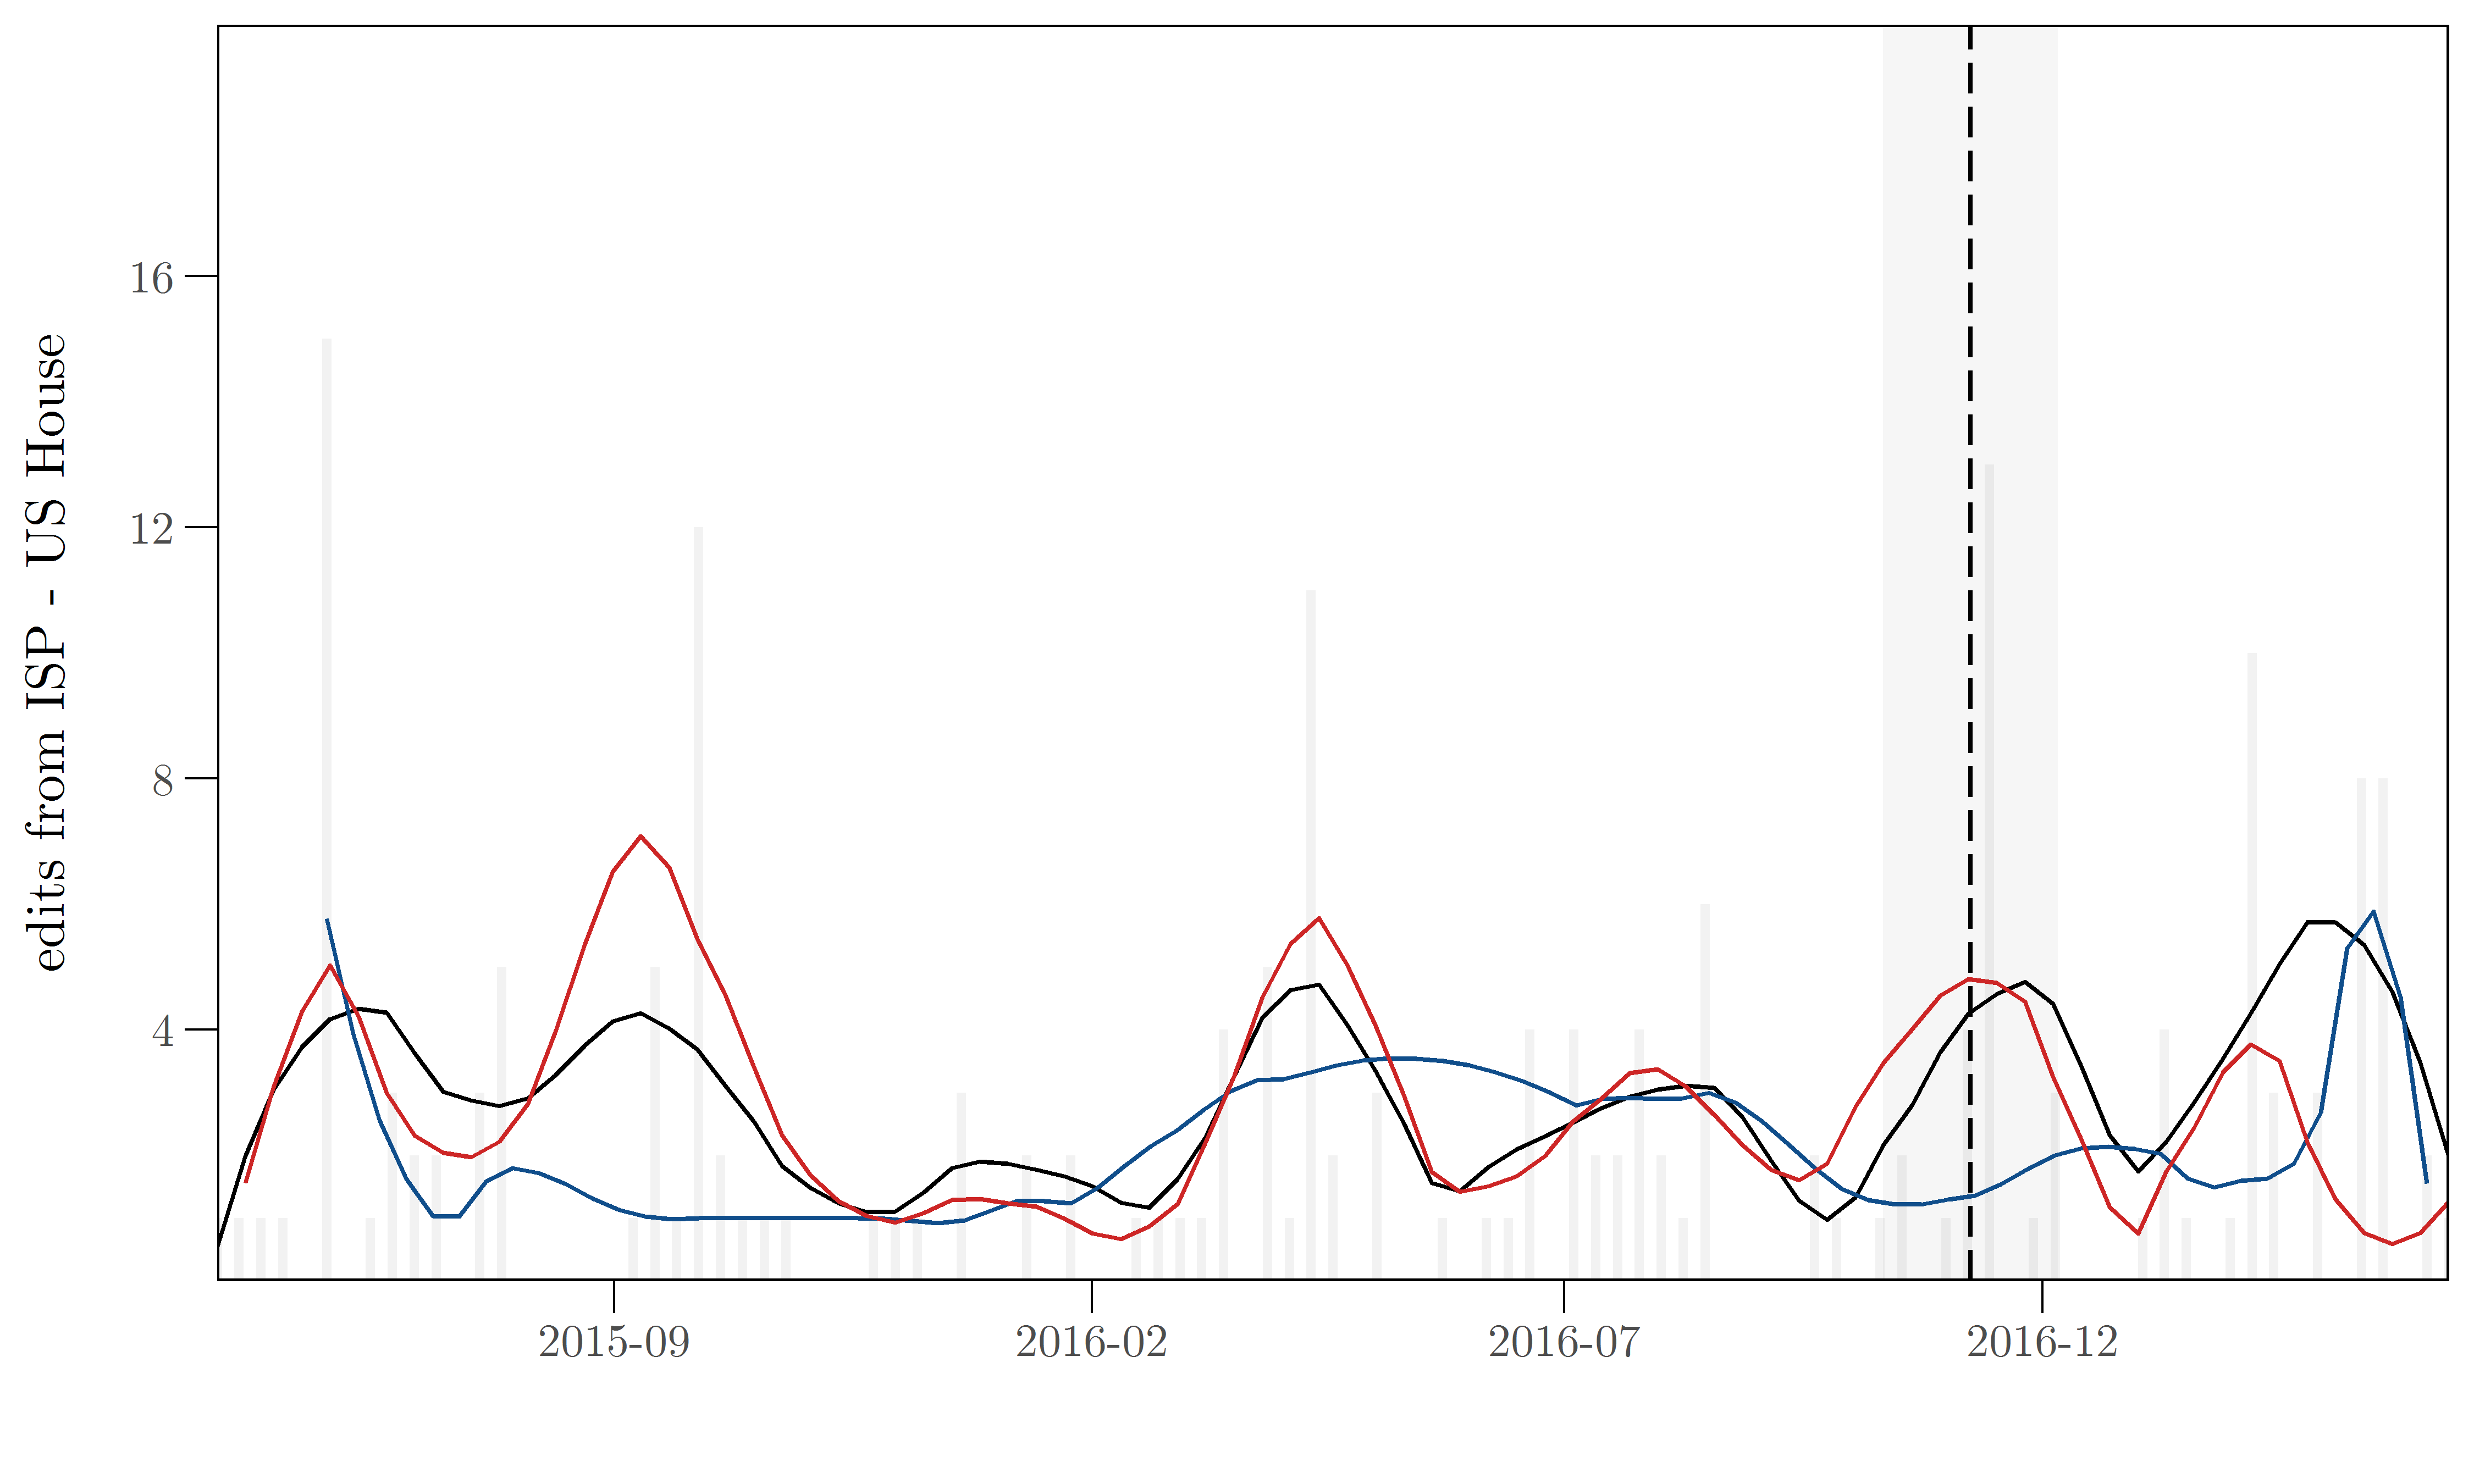
\includegraphics[scale=.55]{uc_2_usah_time2.png}
	\vspace{-.5cm}
\end{center}
\end{figure}
\end{frame}

\begin{frame}{Use Cases (3)}
\begin{figure}[t]
\begin{center}
\vspace{-.1cm}
\hspace*{-0.7cm}
	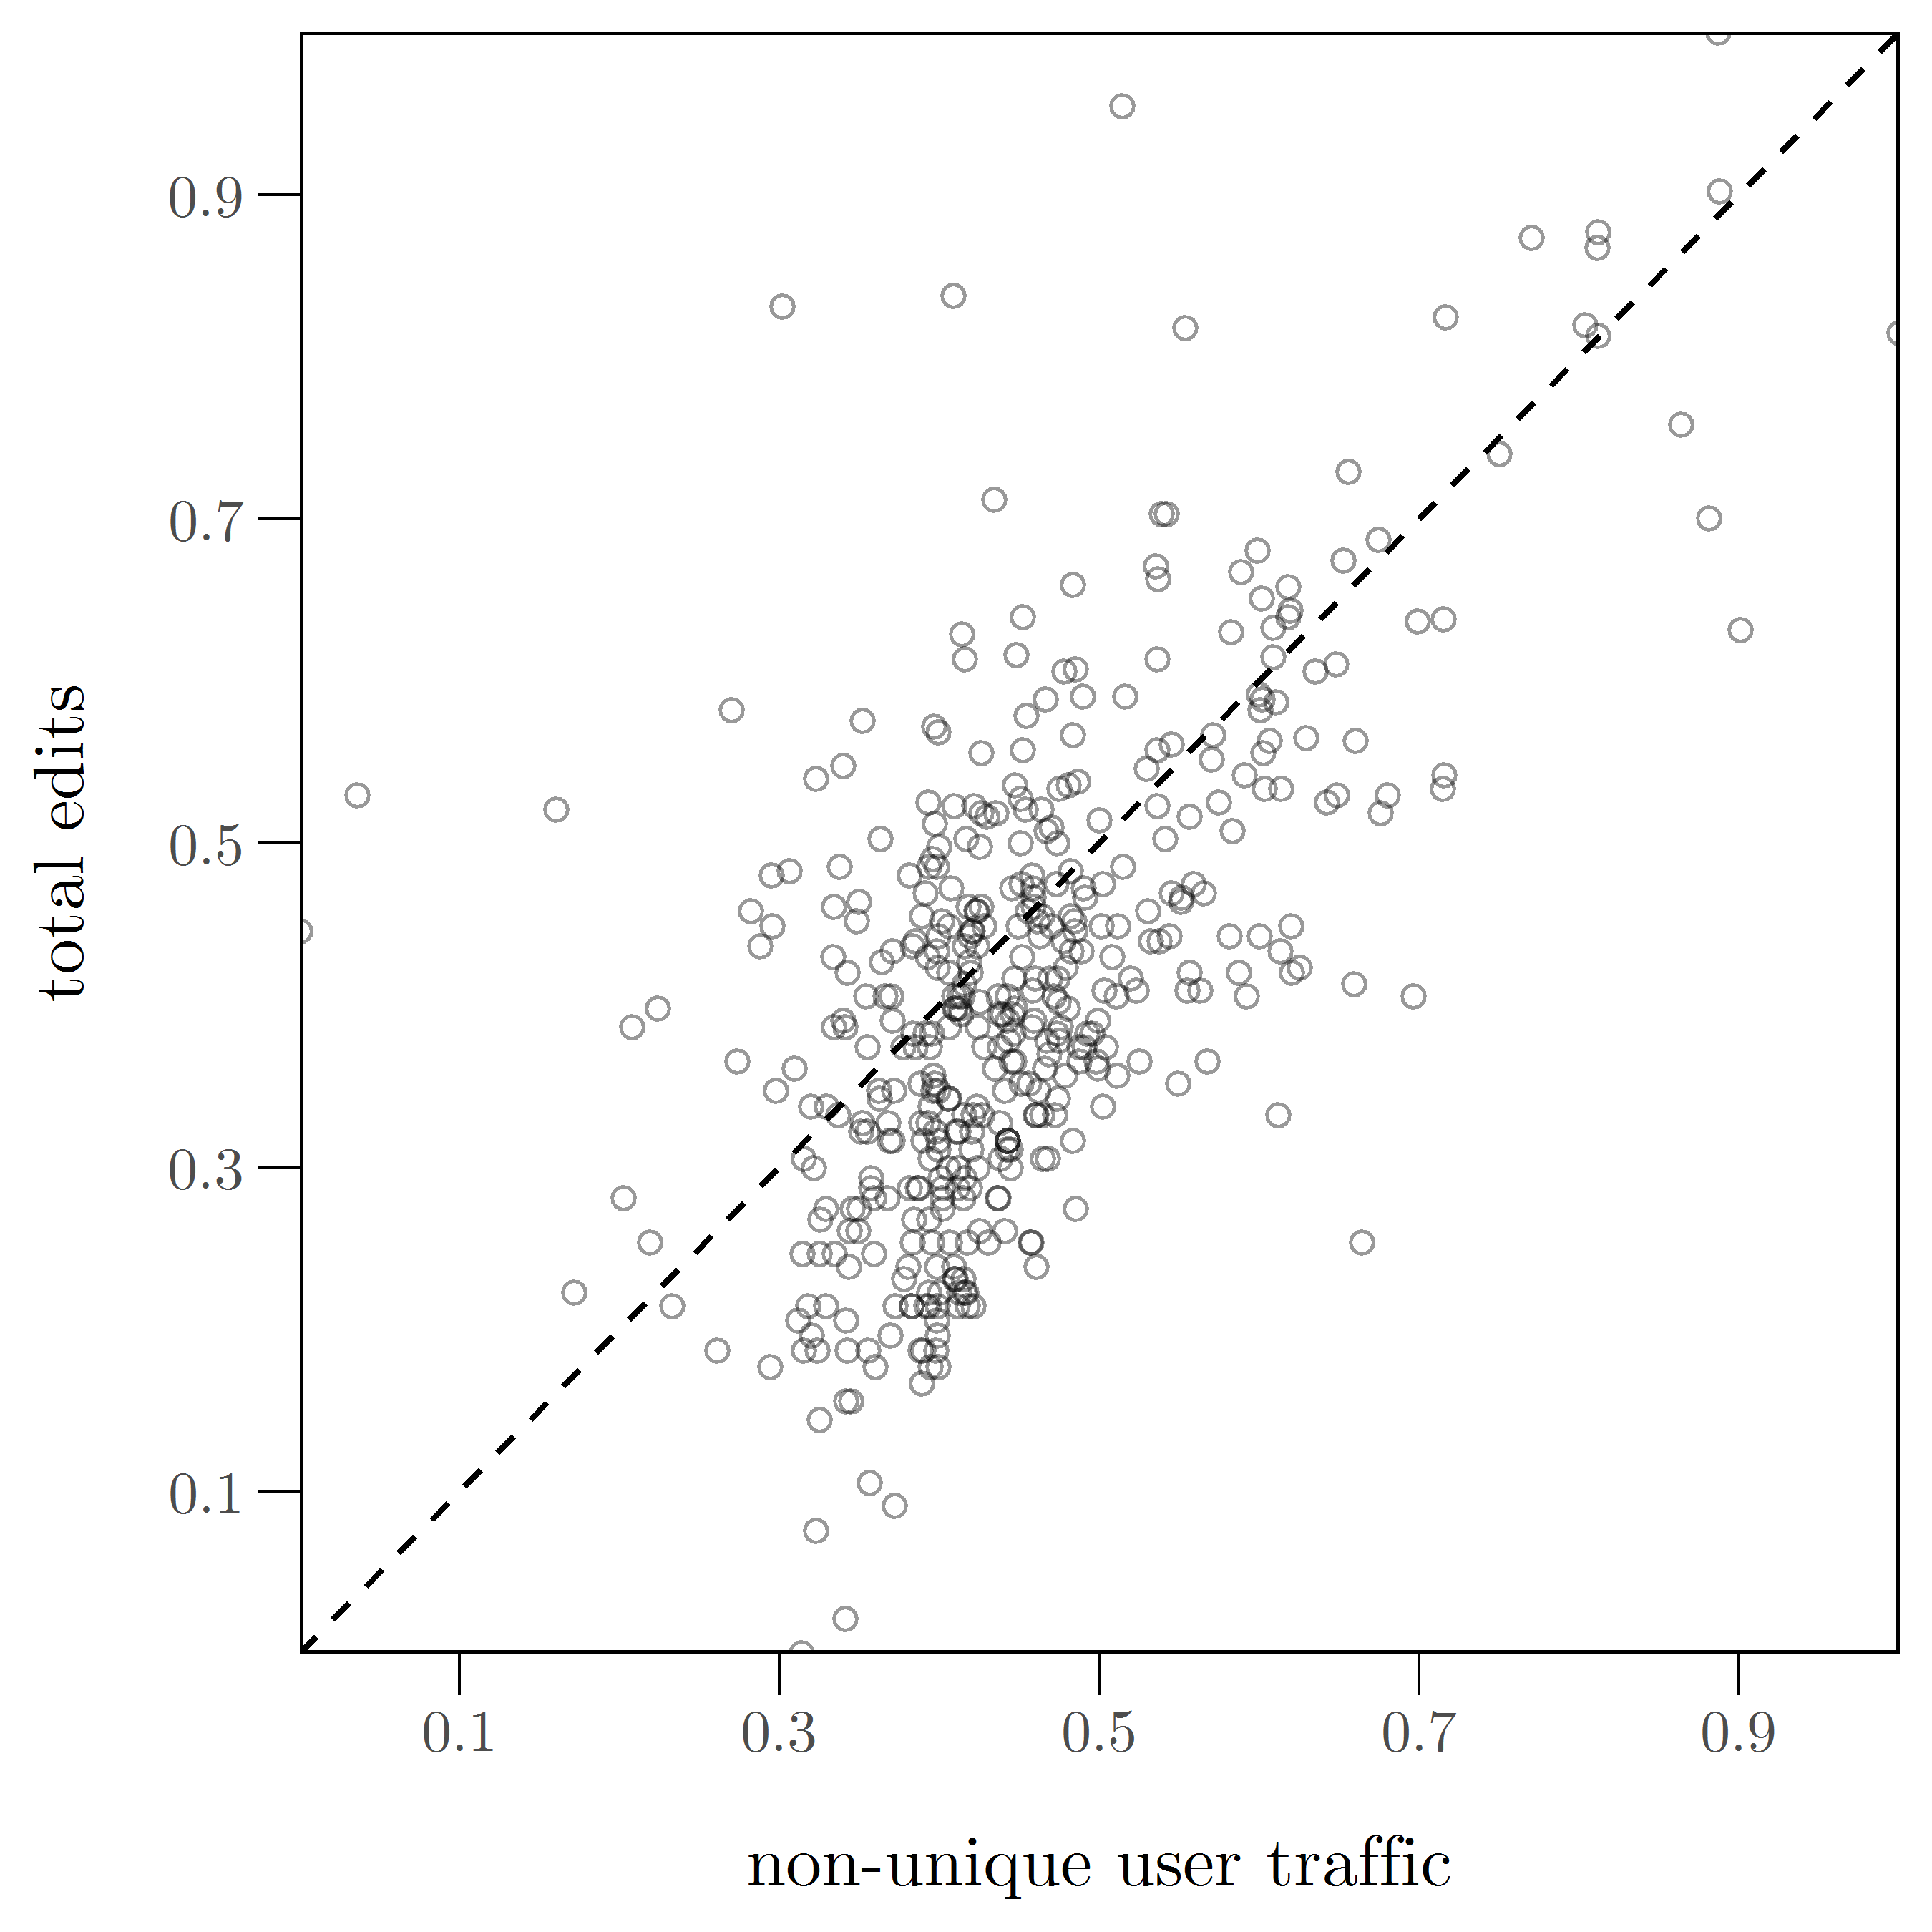
\includegraphics[scale=.5]{uc_3_usah_et.png}
\hspace*{0.5cm}
	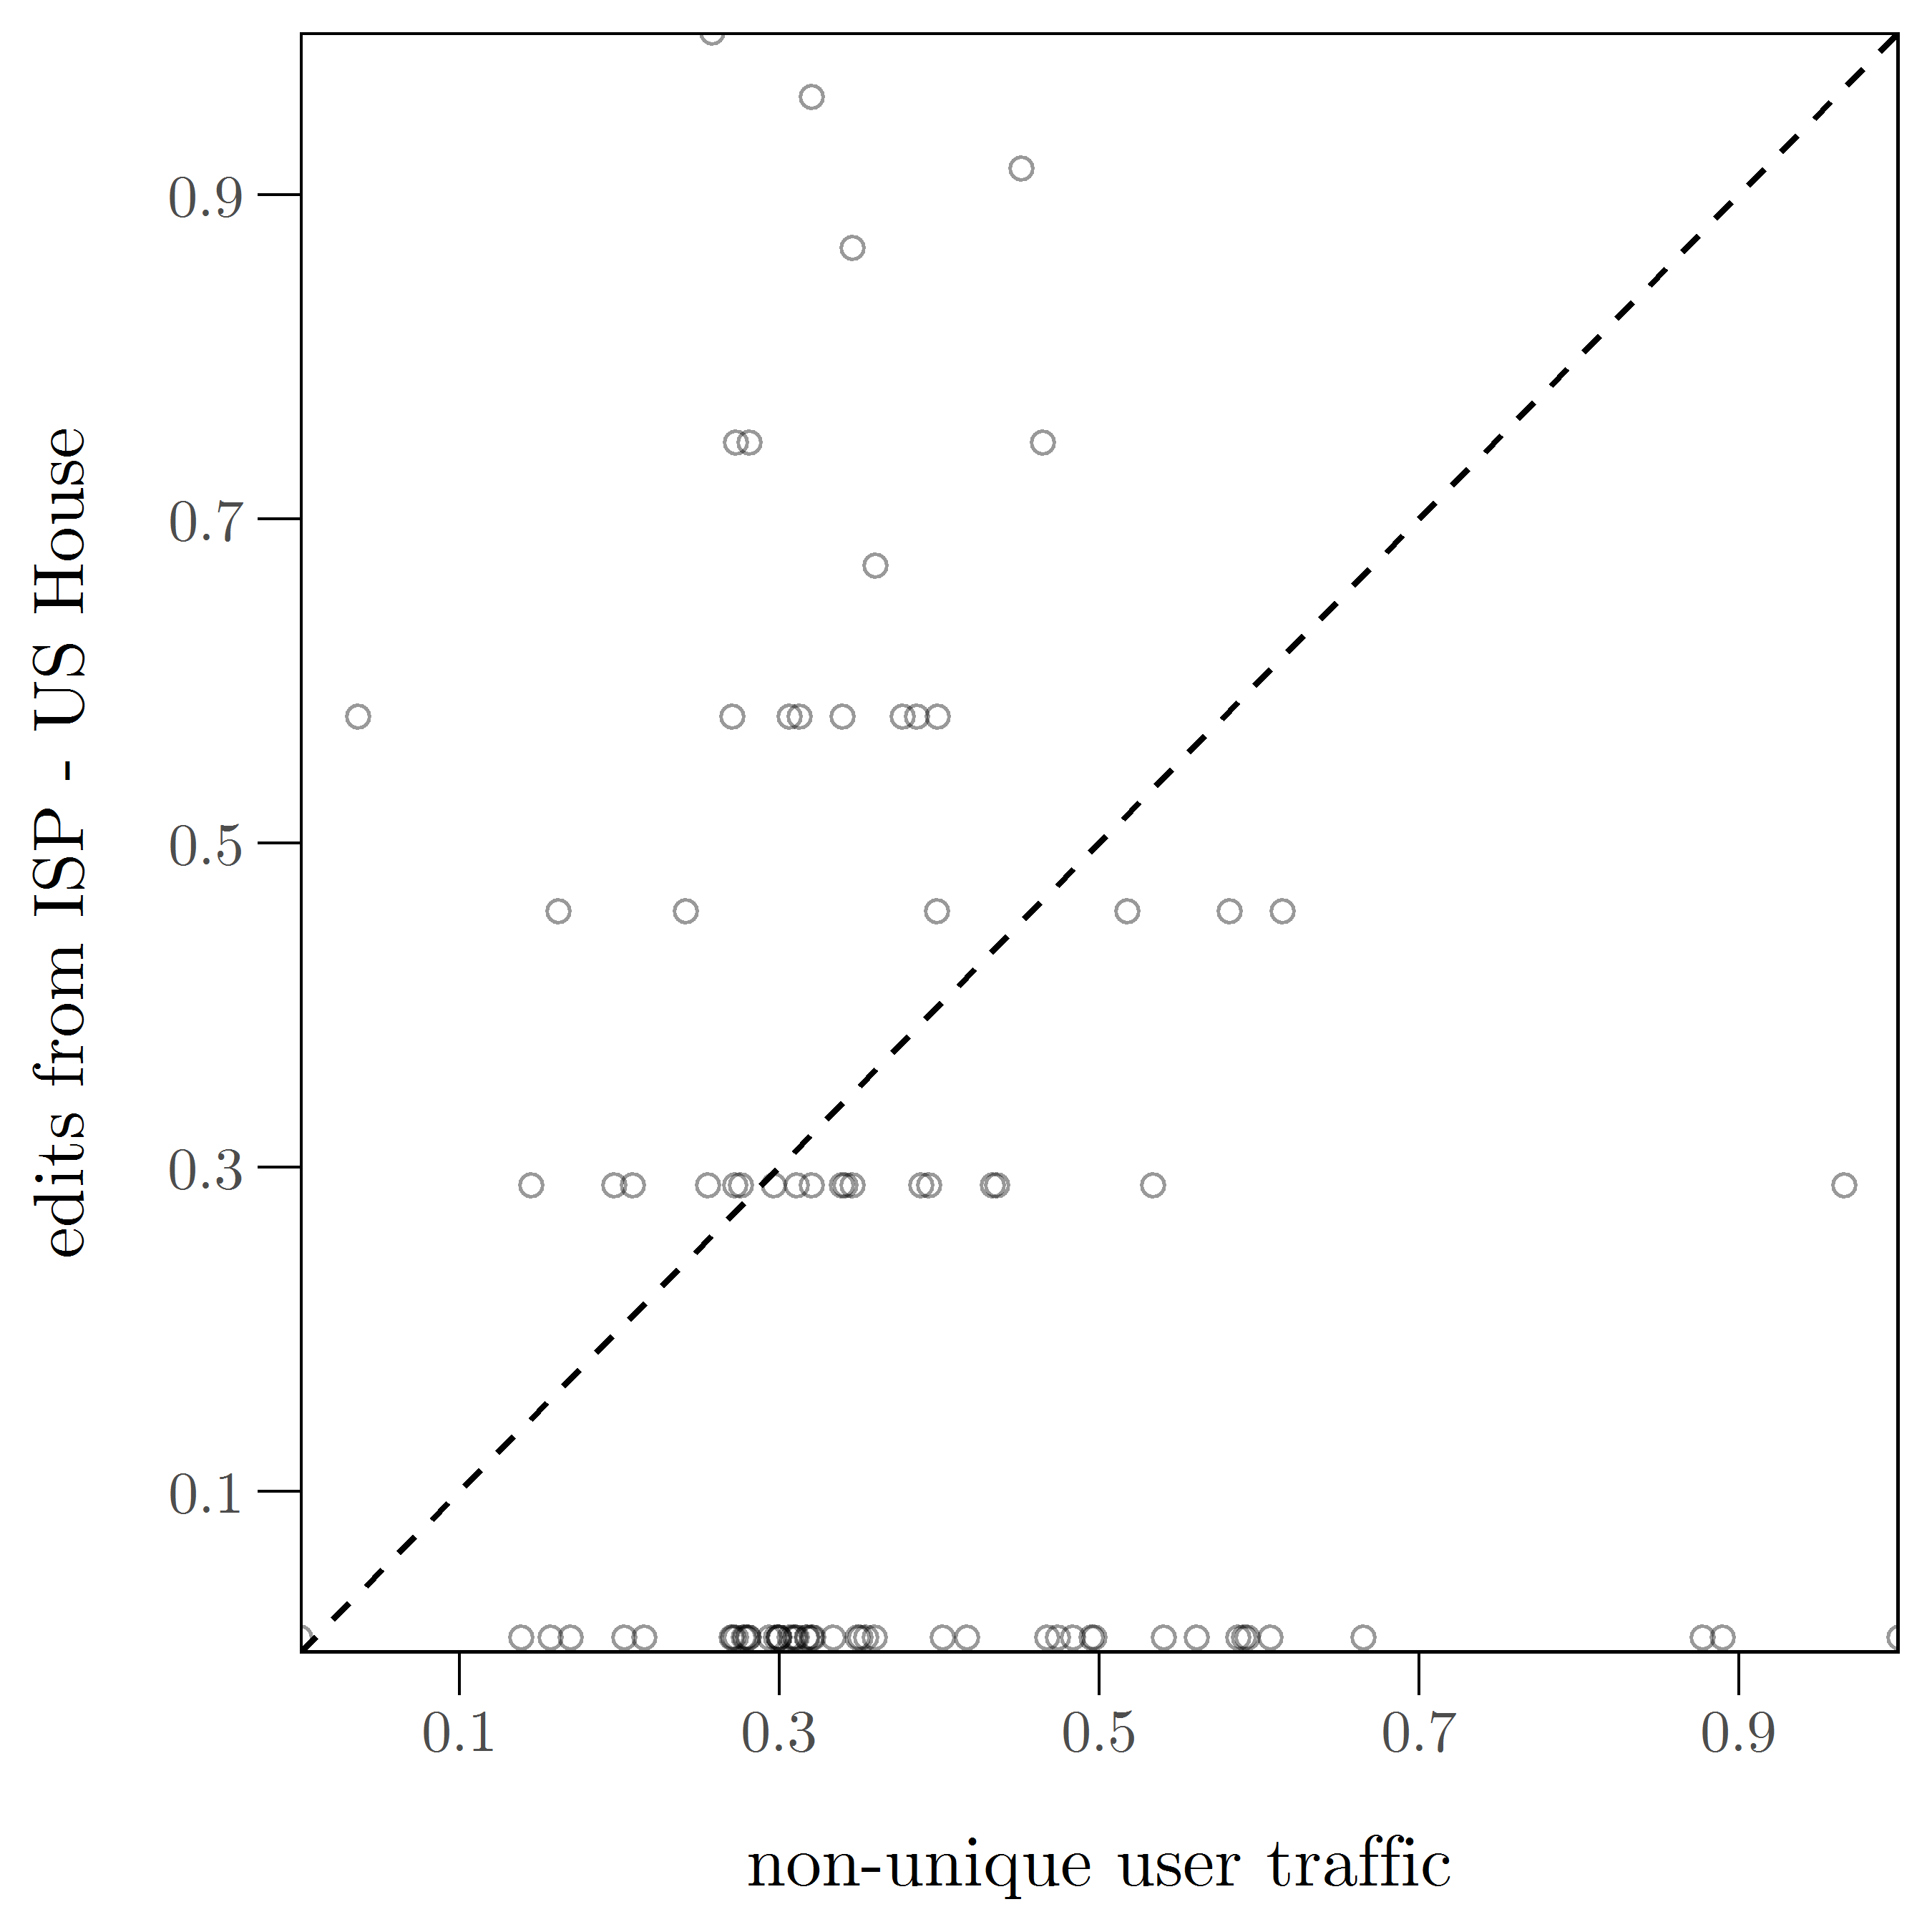
\includegraphics[scale=.5]{uc_3_usah_et2.png}
	\vspace{-.5cm}
\end{center}
\end{figure}
\end{frame}

\begin{frame}{Use Cases (4)}
\begin{figure}[t]
\begin{center}
\vspace{-.1cm}
	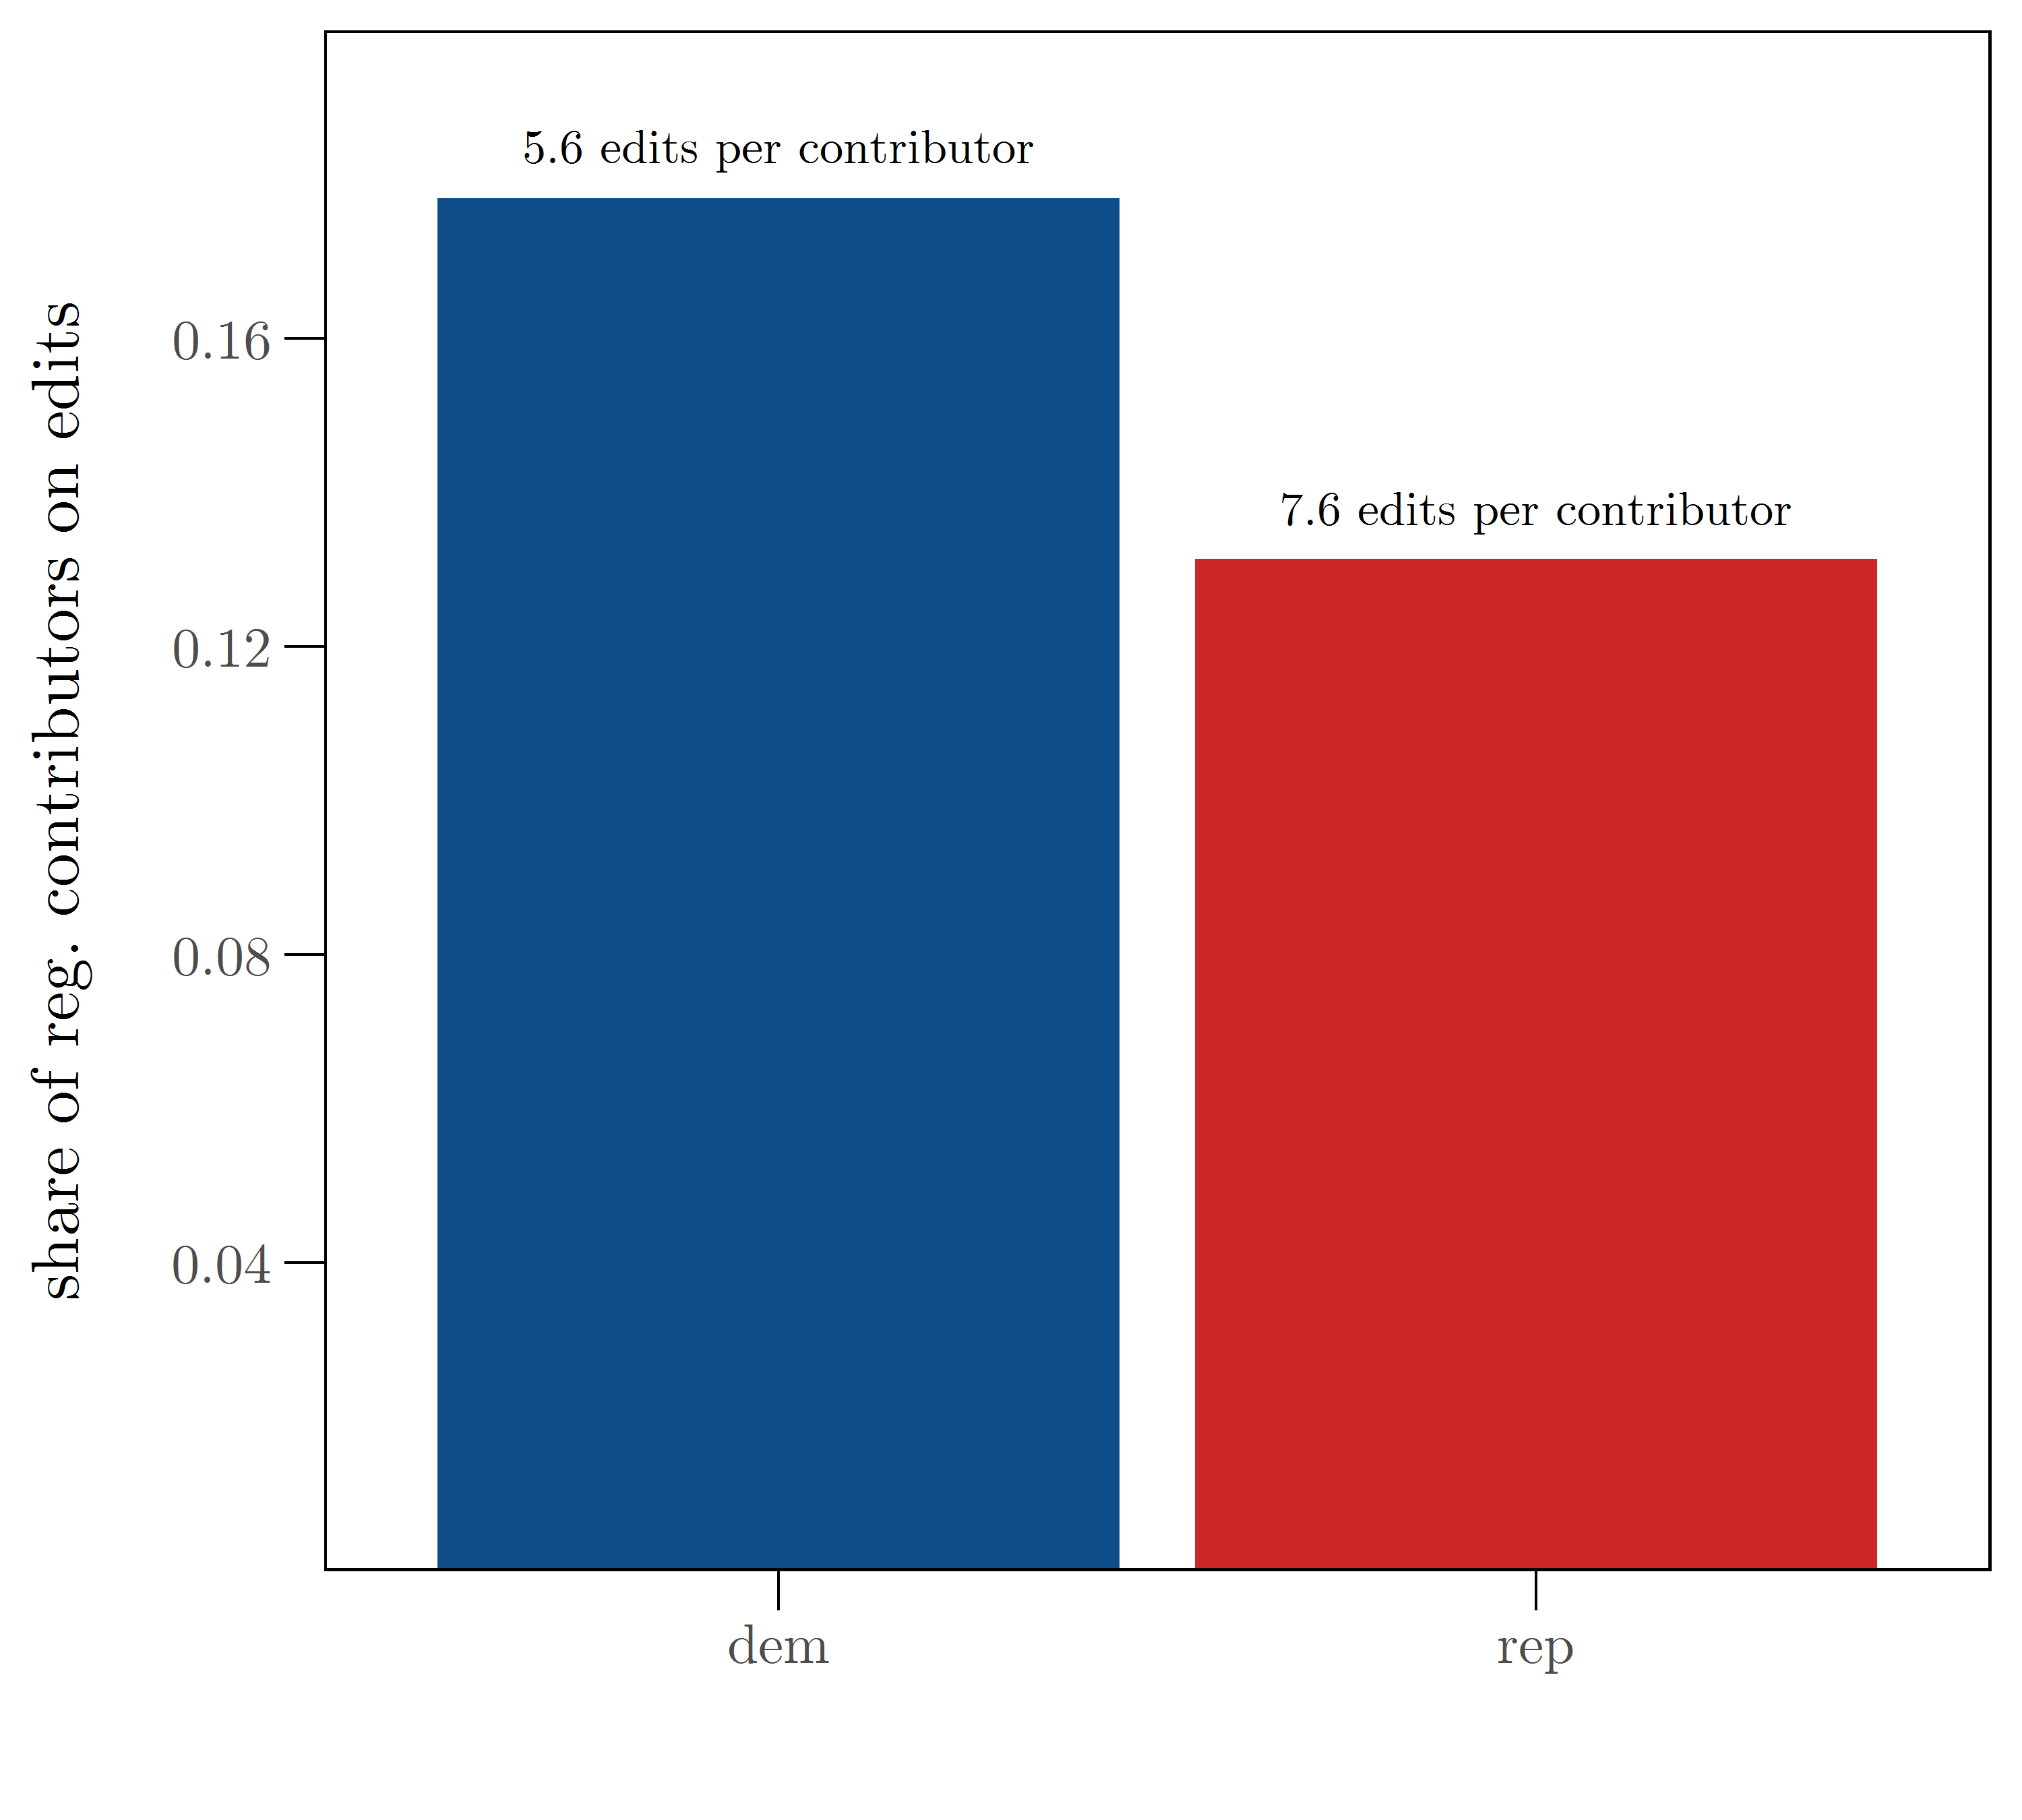
\includegraphics[scale=.63]{uc_4_usah_cont1.png}
	\vspace{-.5cm}
\end{center}
\end{figure}
\end{frame}

\begin{frame}{Use Cases (4)}
\begin{figure}[t]
\begin{center}
\vspace{-.1cm}
\hspace*{-0.95cm}
	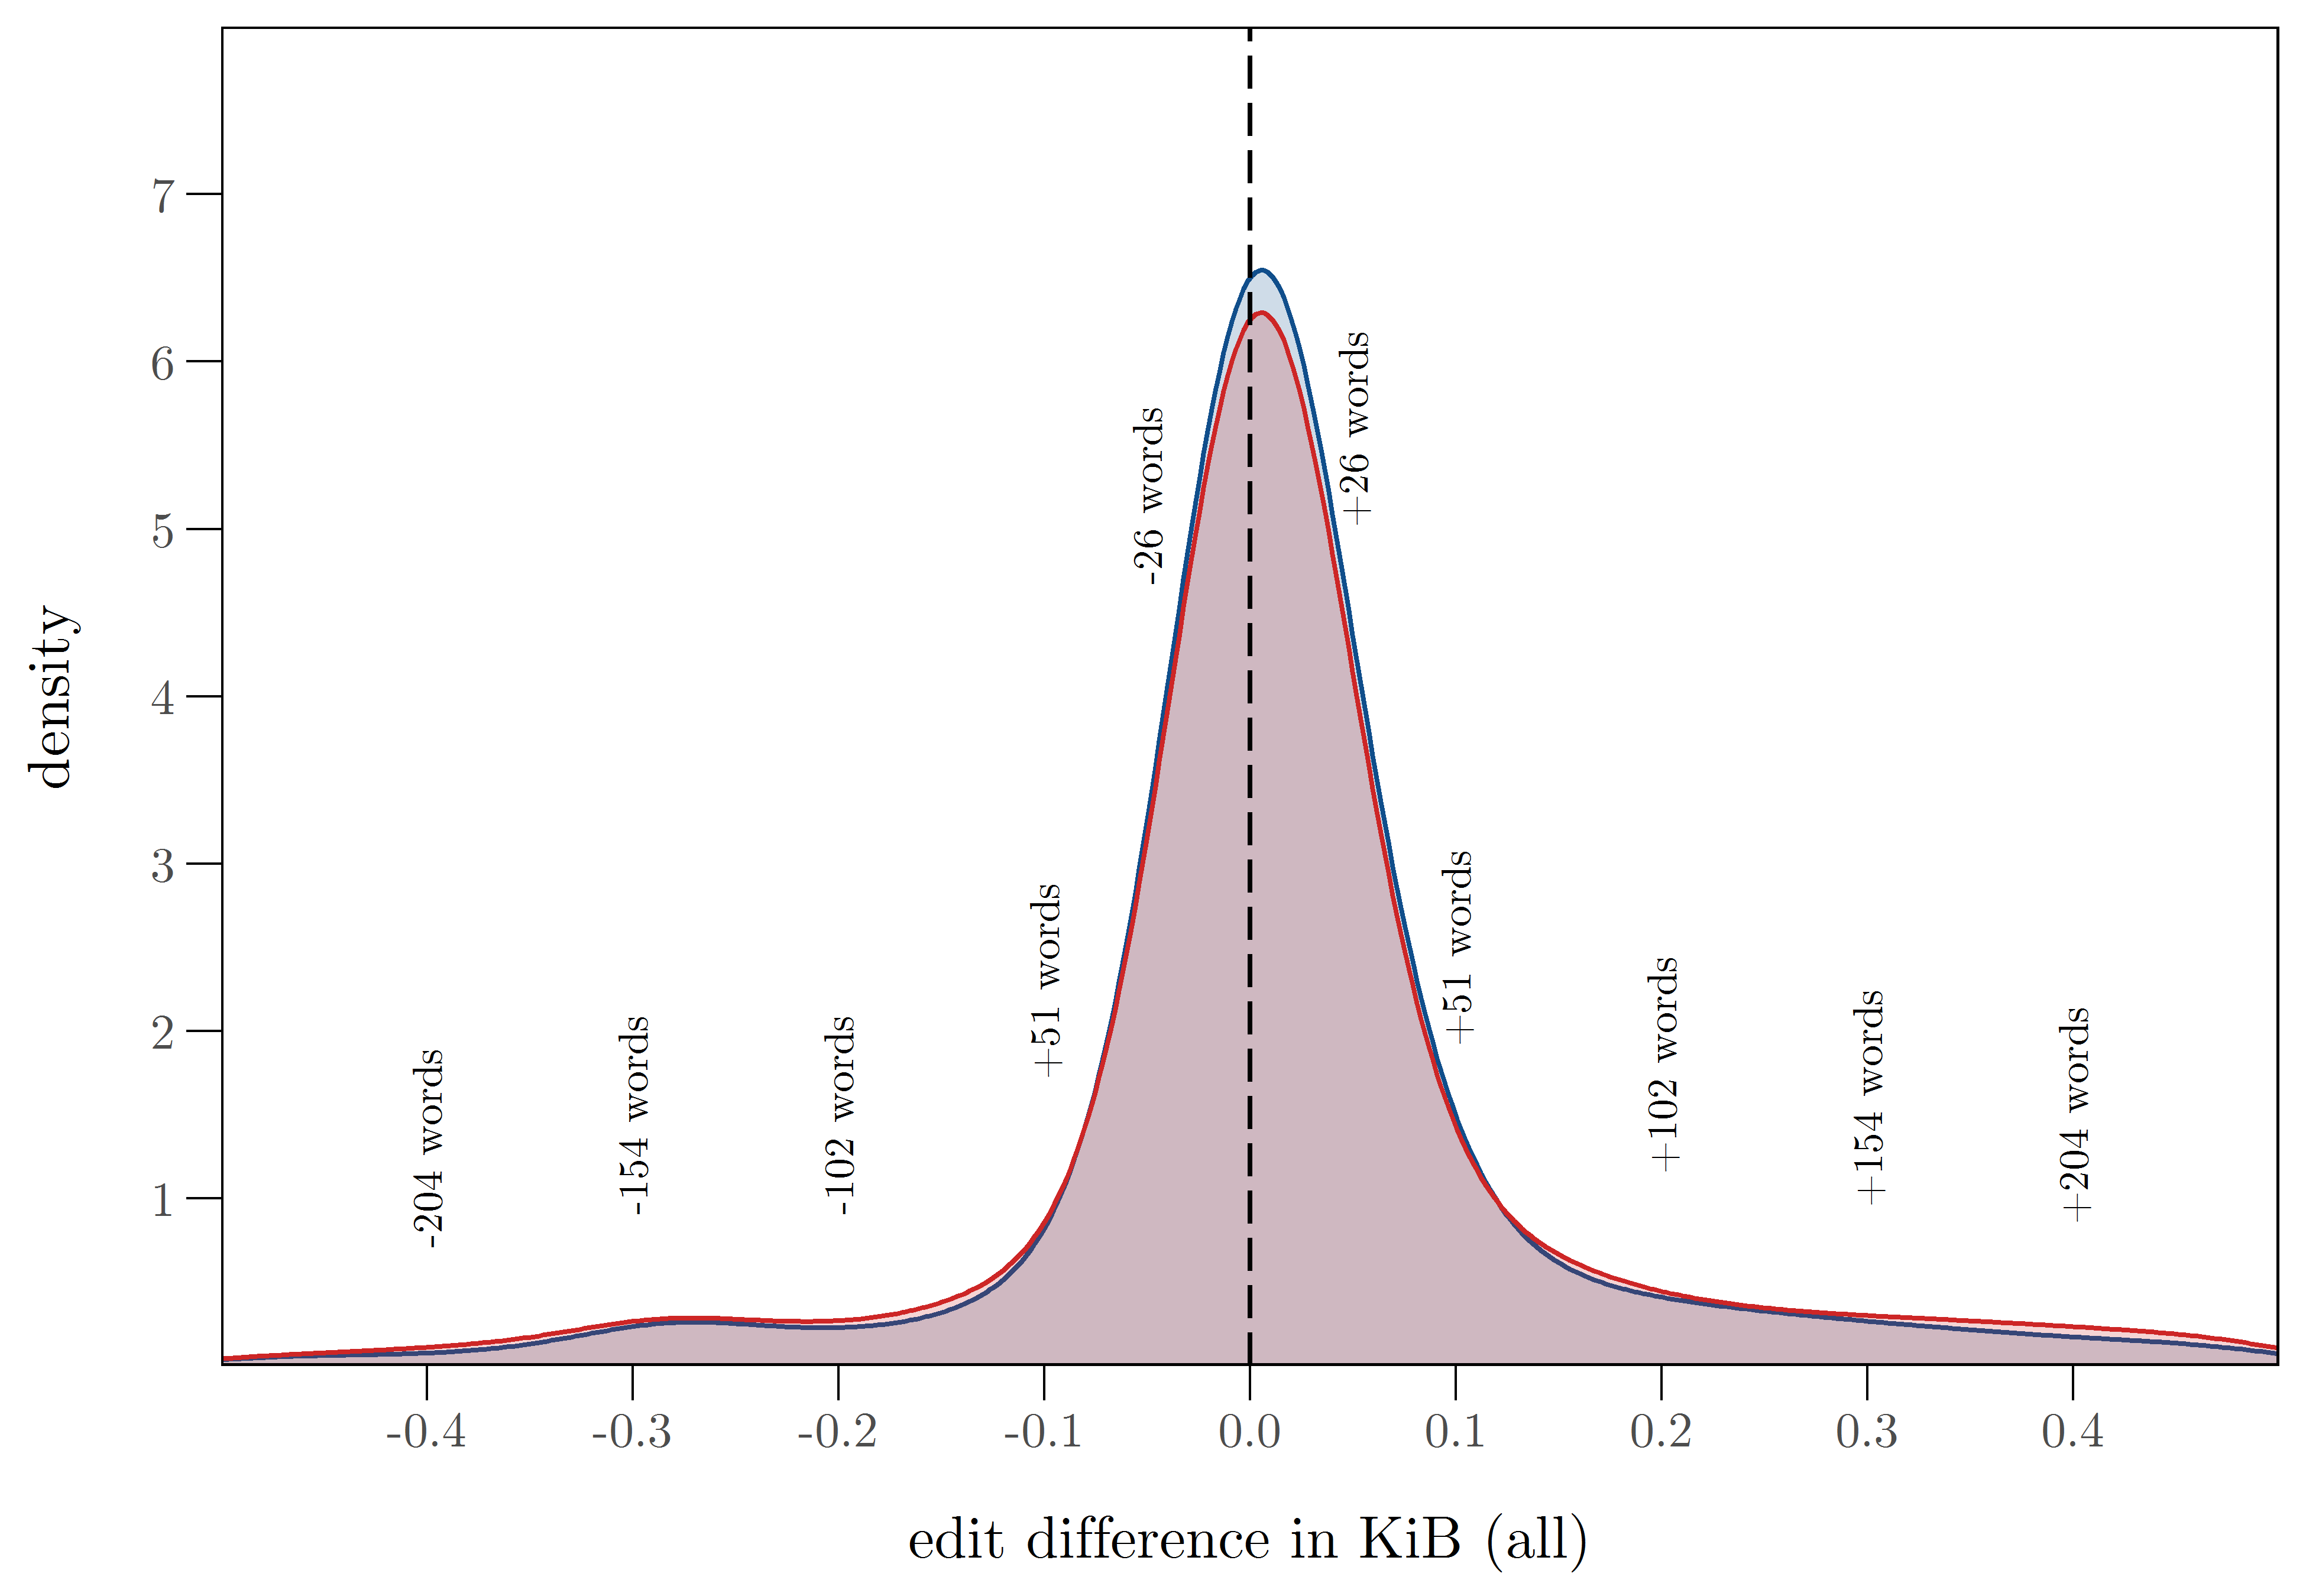
\includegraphics[scale=.38]{uc_4_usah_cont2.png}
\hspace*{-0.1cm}
	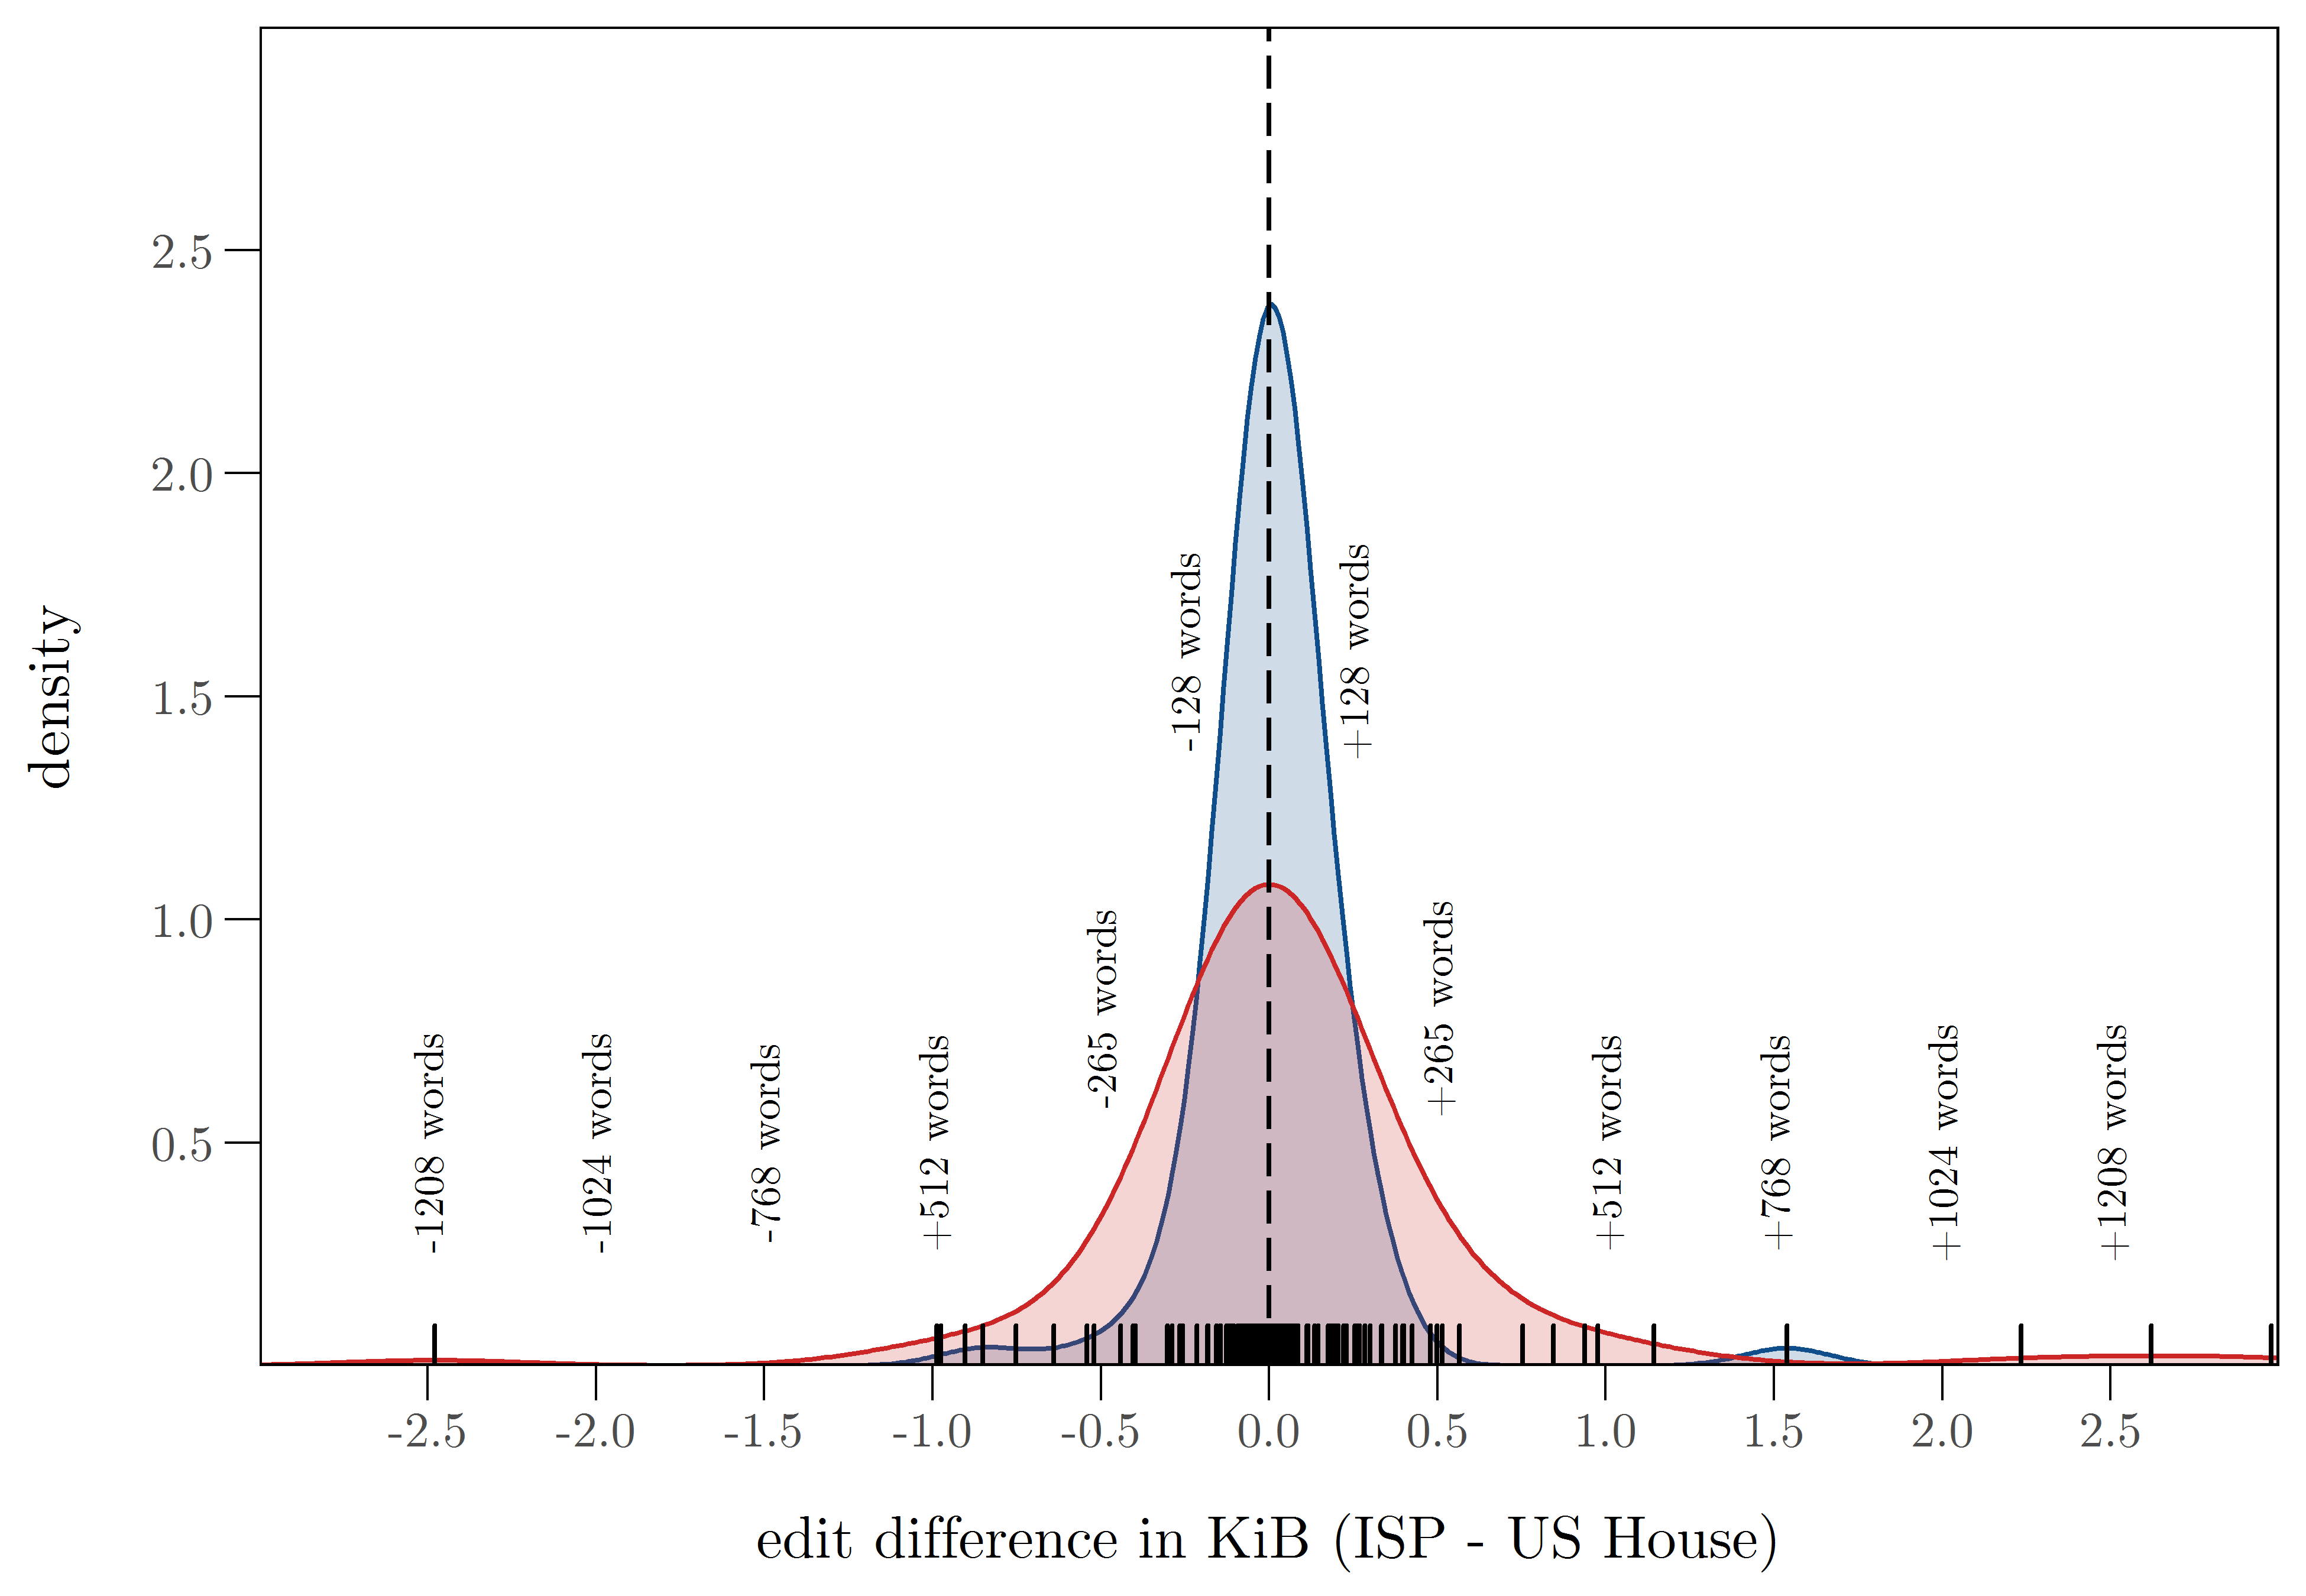
\includegraphics[scale=.38]{uc_4_usah_cont3.png}
	\vspace{-.5cm}
\end{center}
\end{figure}
\end{frame}

\begin{frame}{Use Cases (5)}
\begin{figure}[t]
\begin{center}
\vspace{-.5cm}
\hspace*{-0.8cm}
	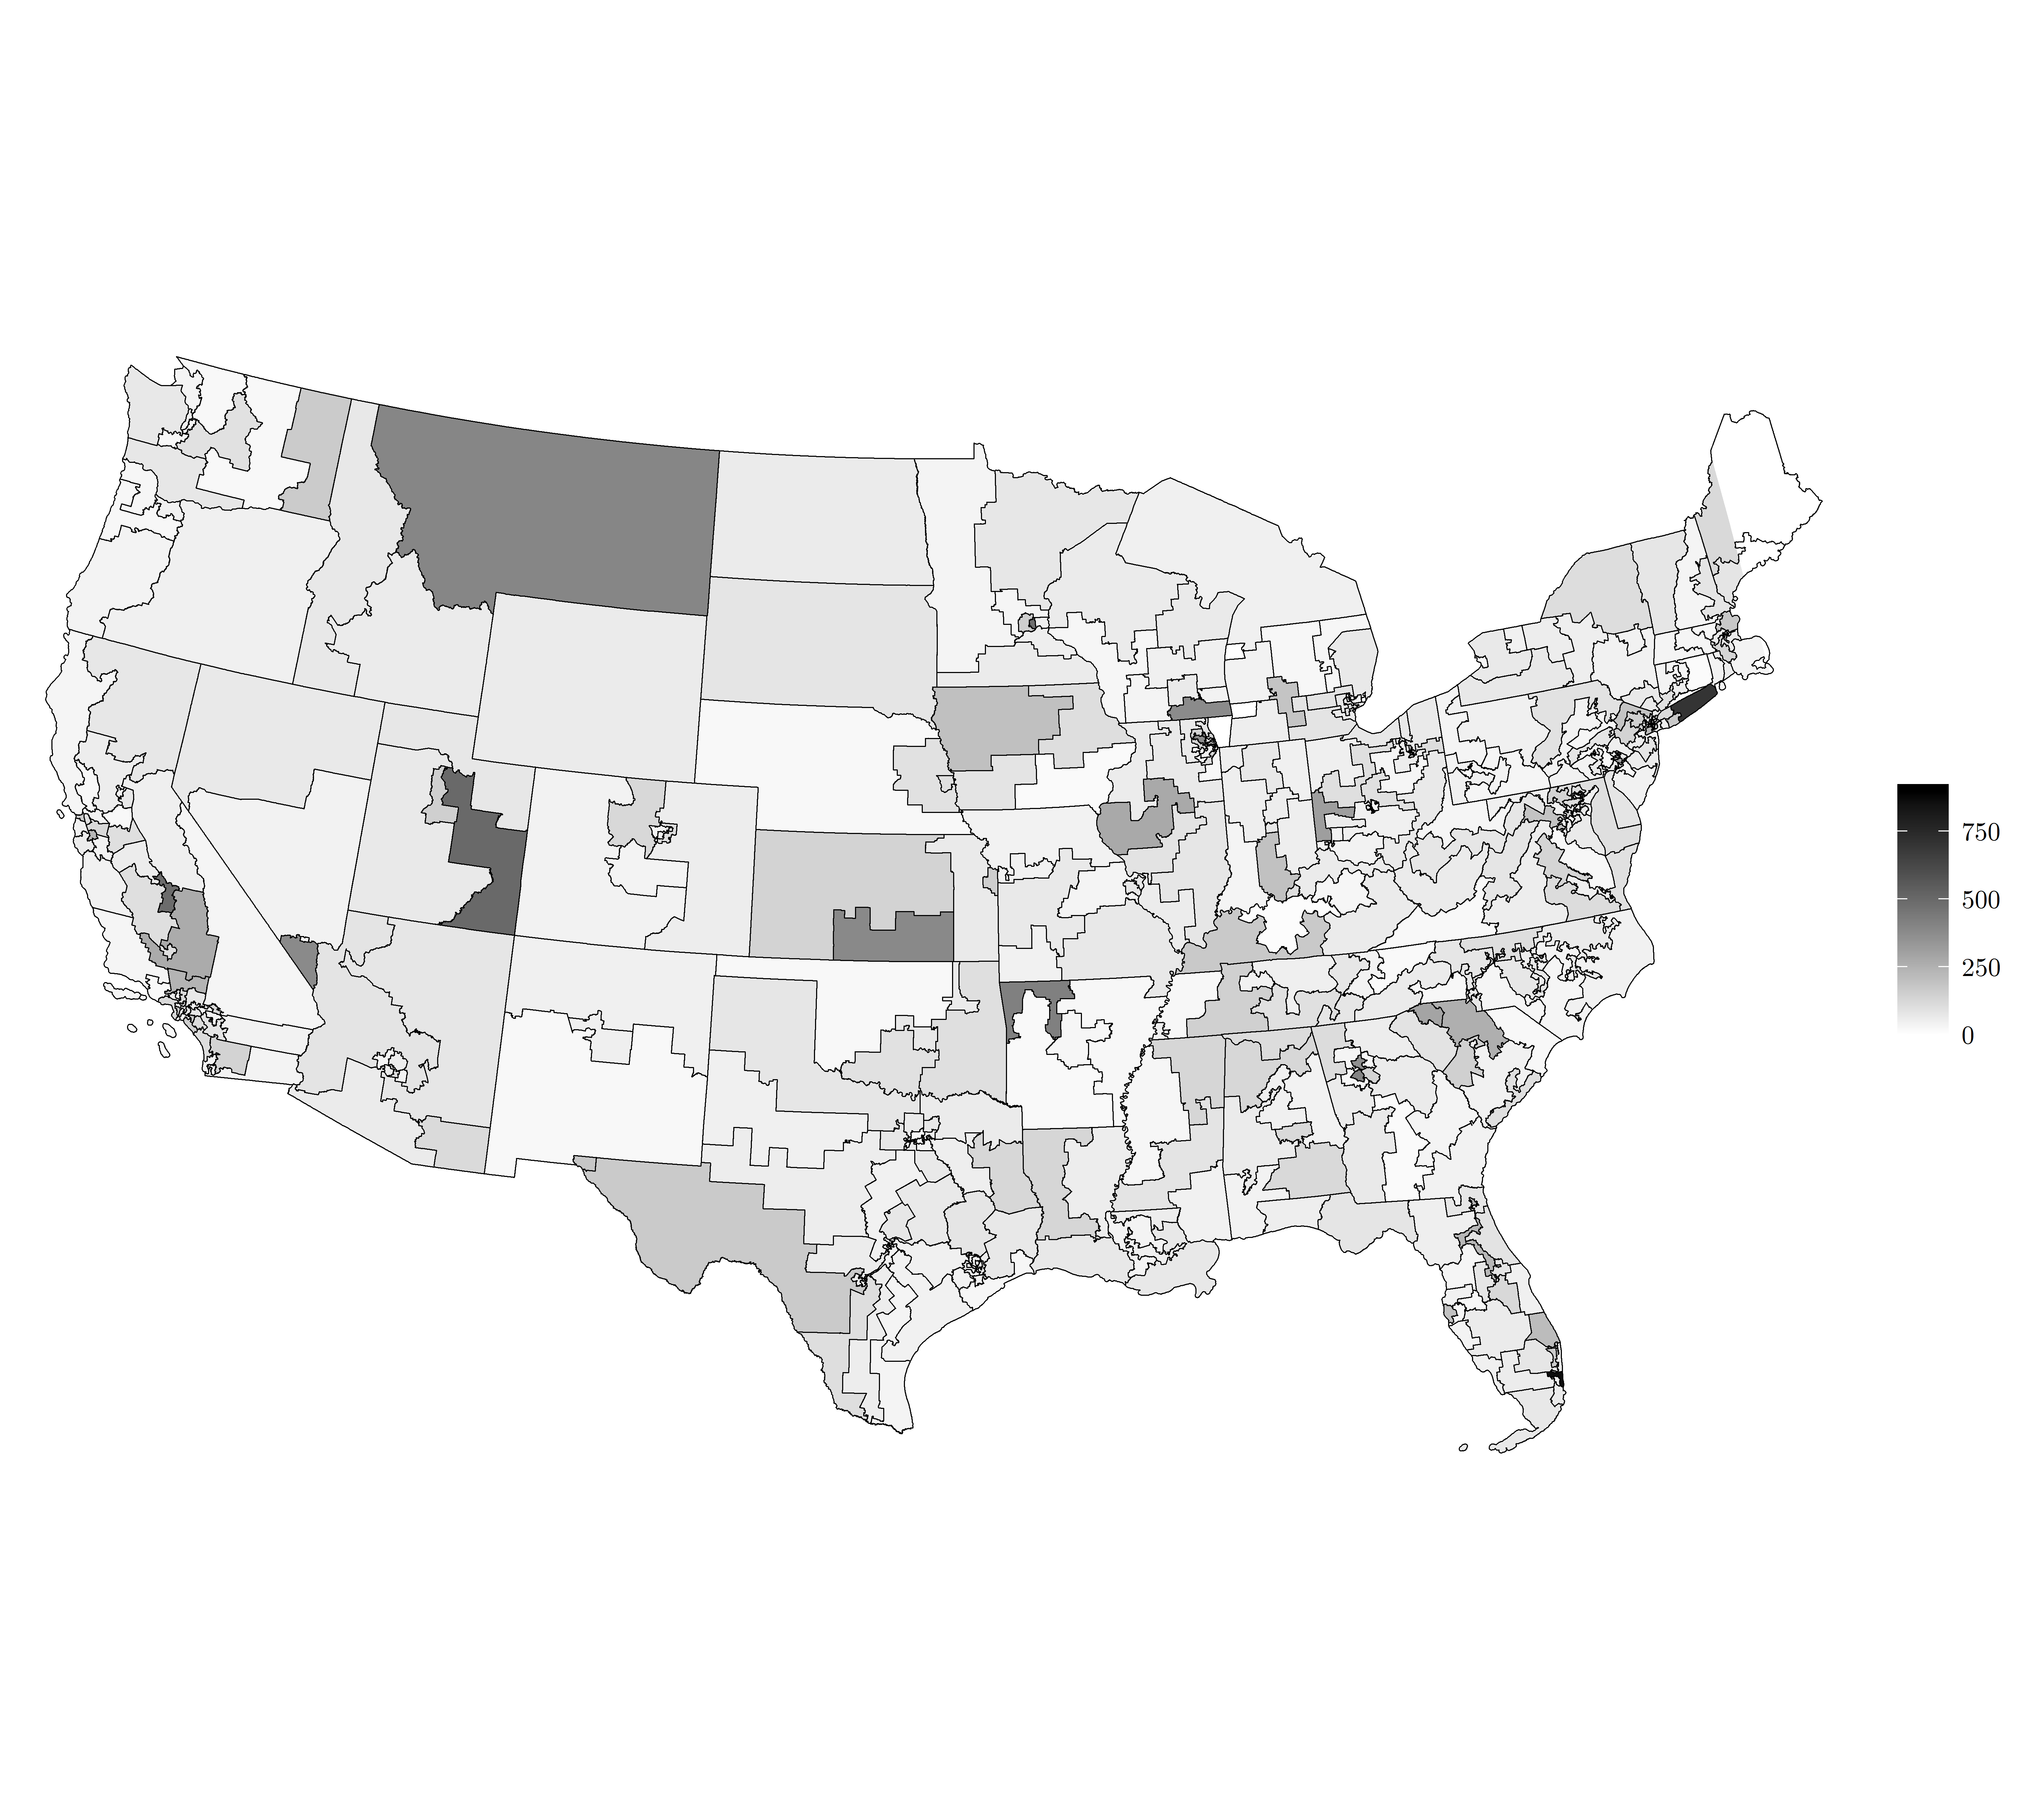
\includegraphics[scale=.17]{uc_5_map_edits1.png}
\hspace*{-0.1cm}
	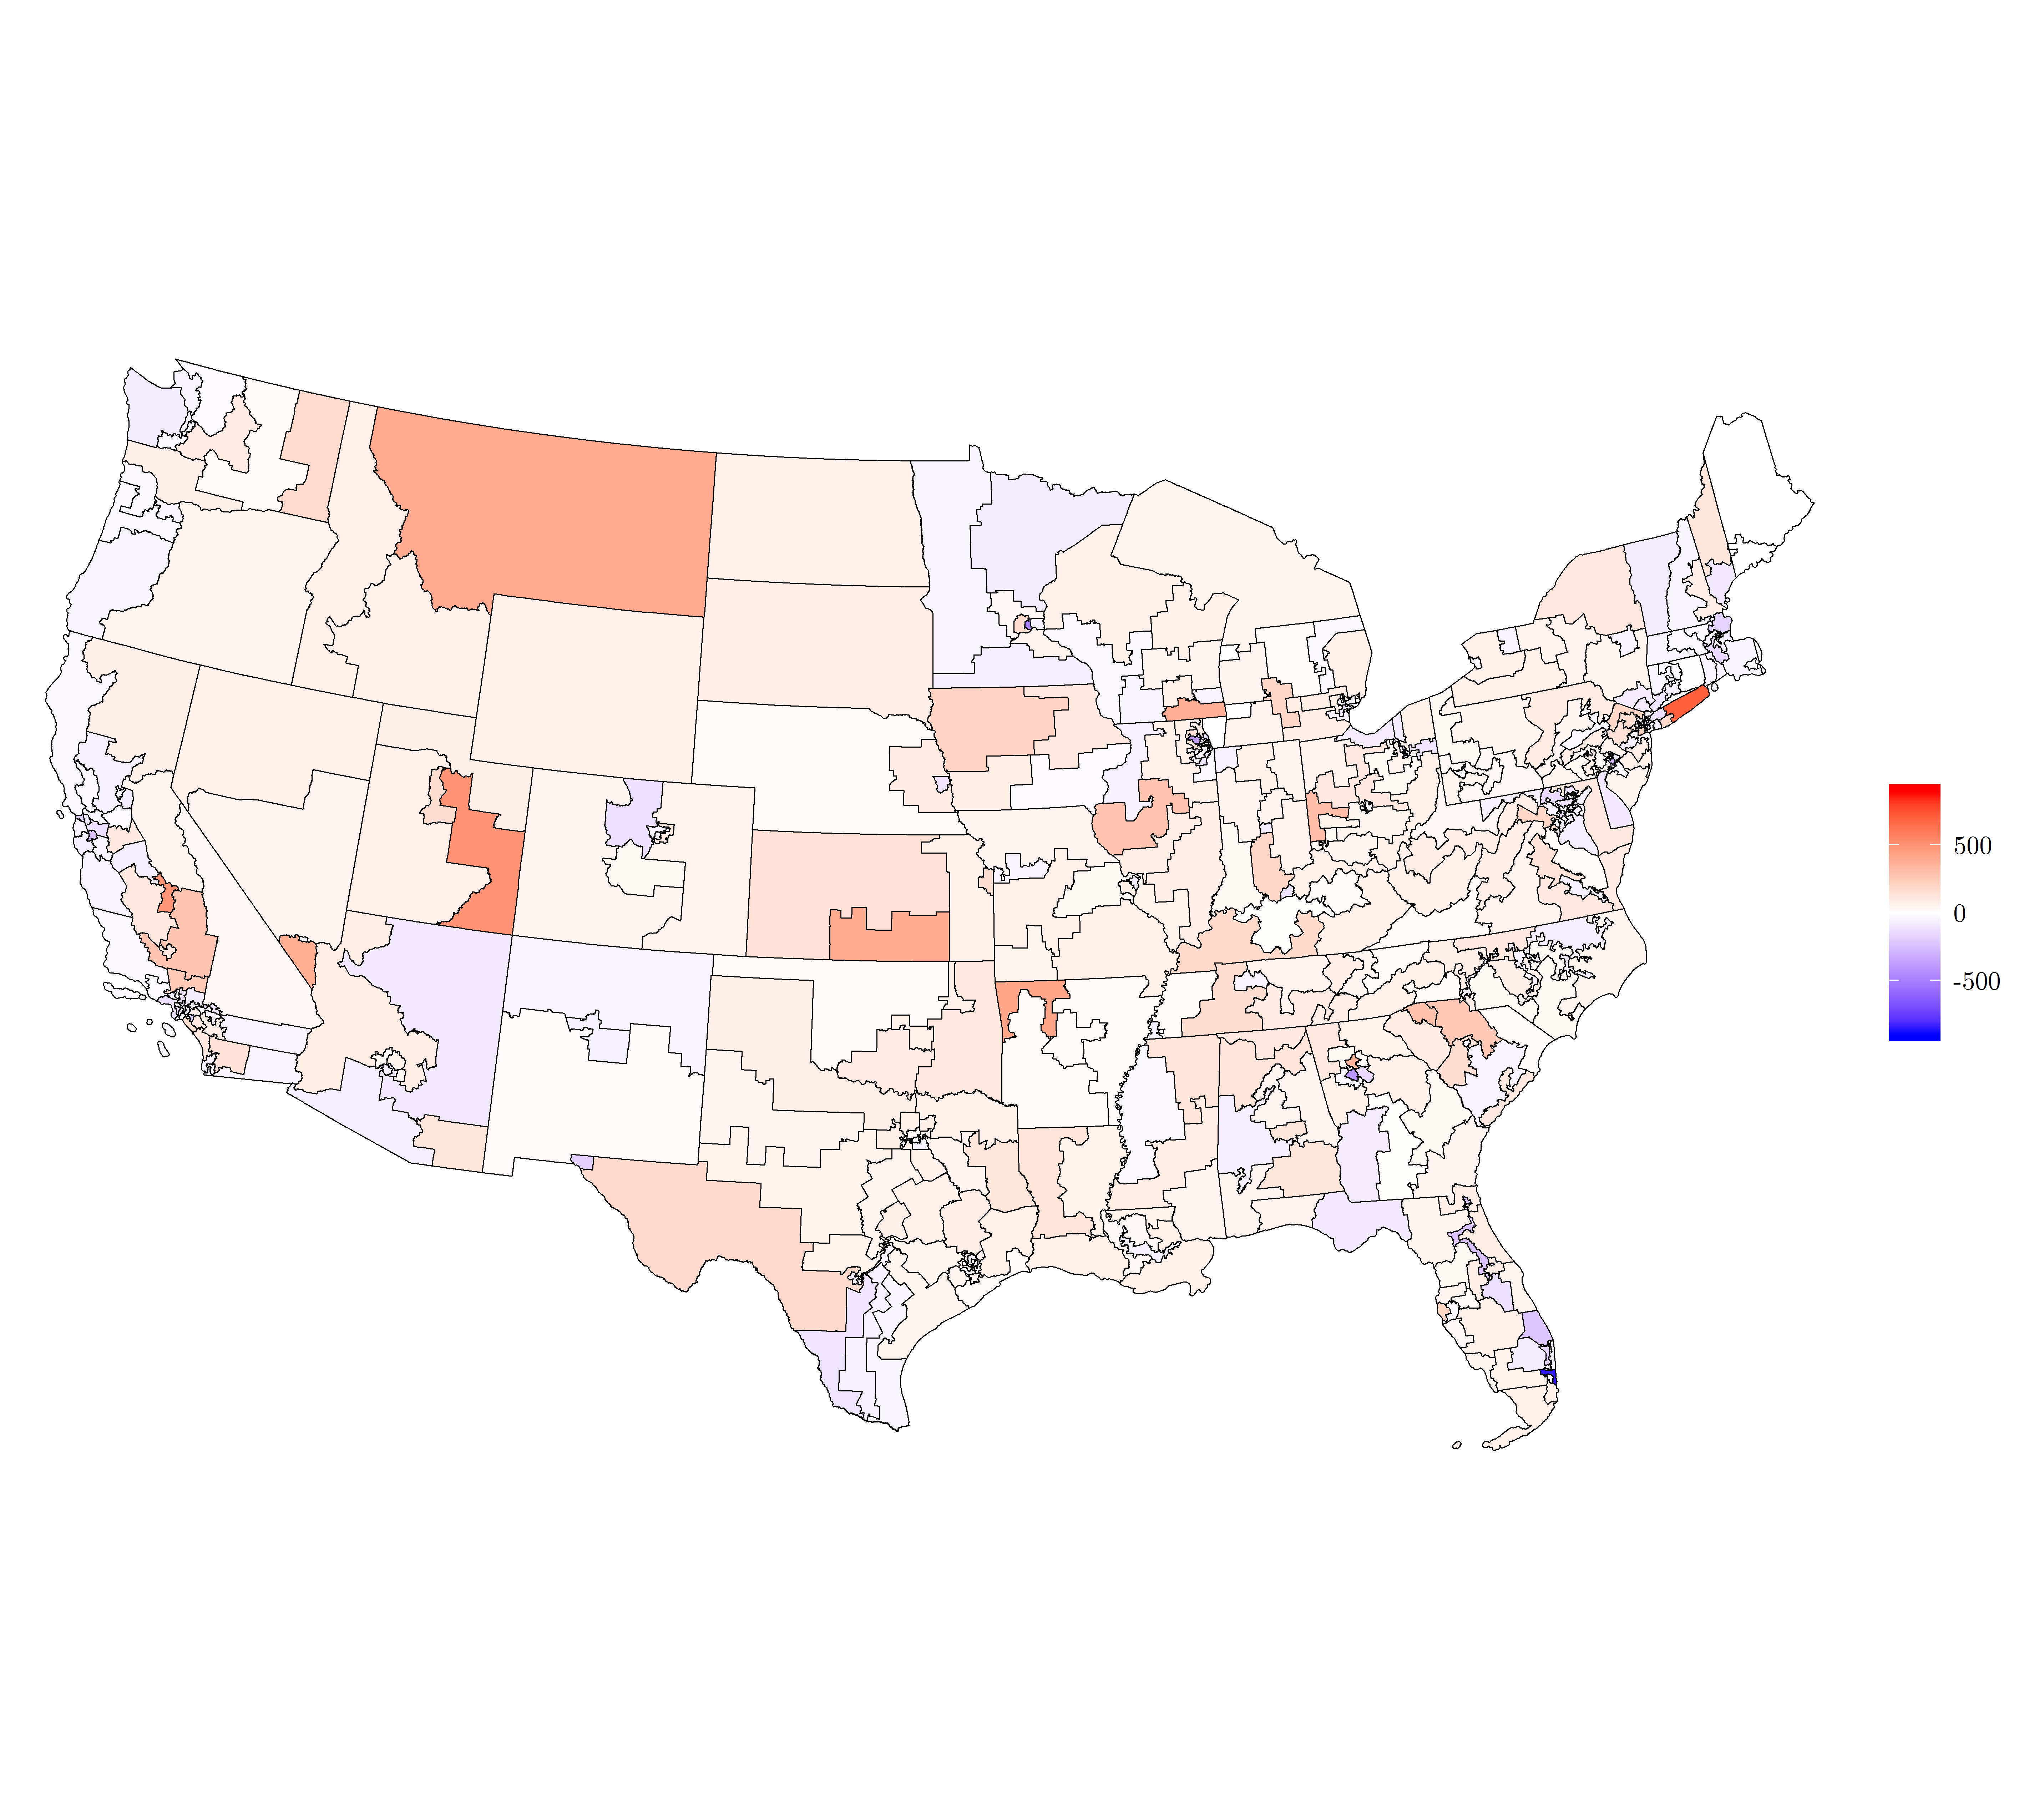
\includegraphics[scale=.17]{uc_5_map_edits2.png}
	\hspace*{-0.1cm}
	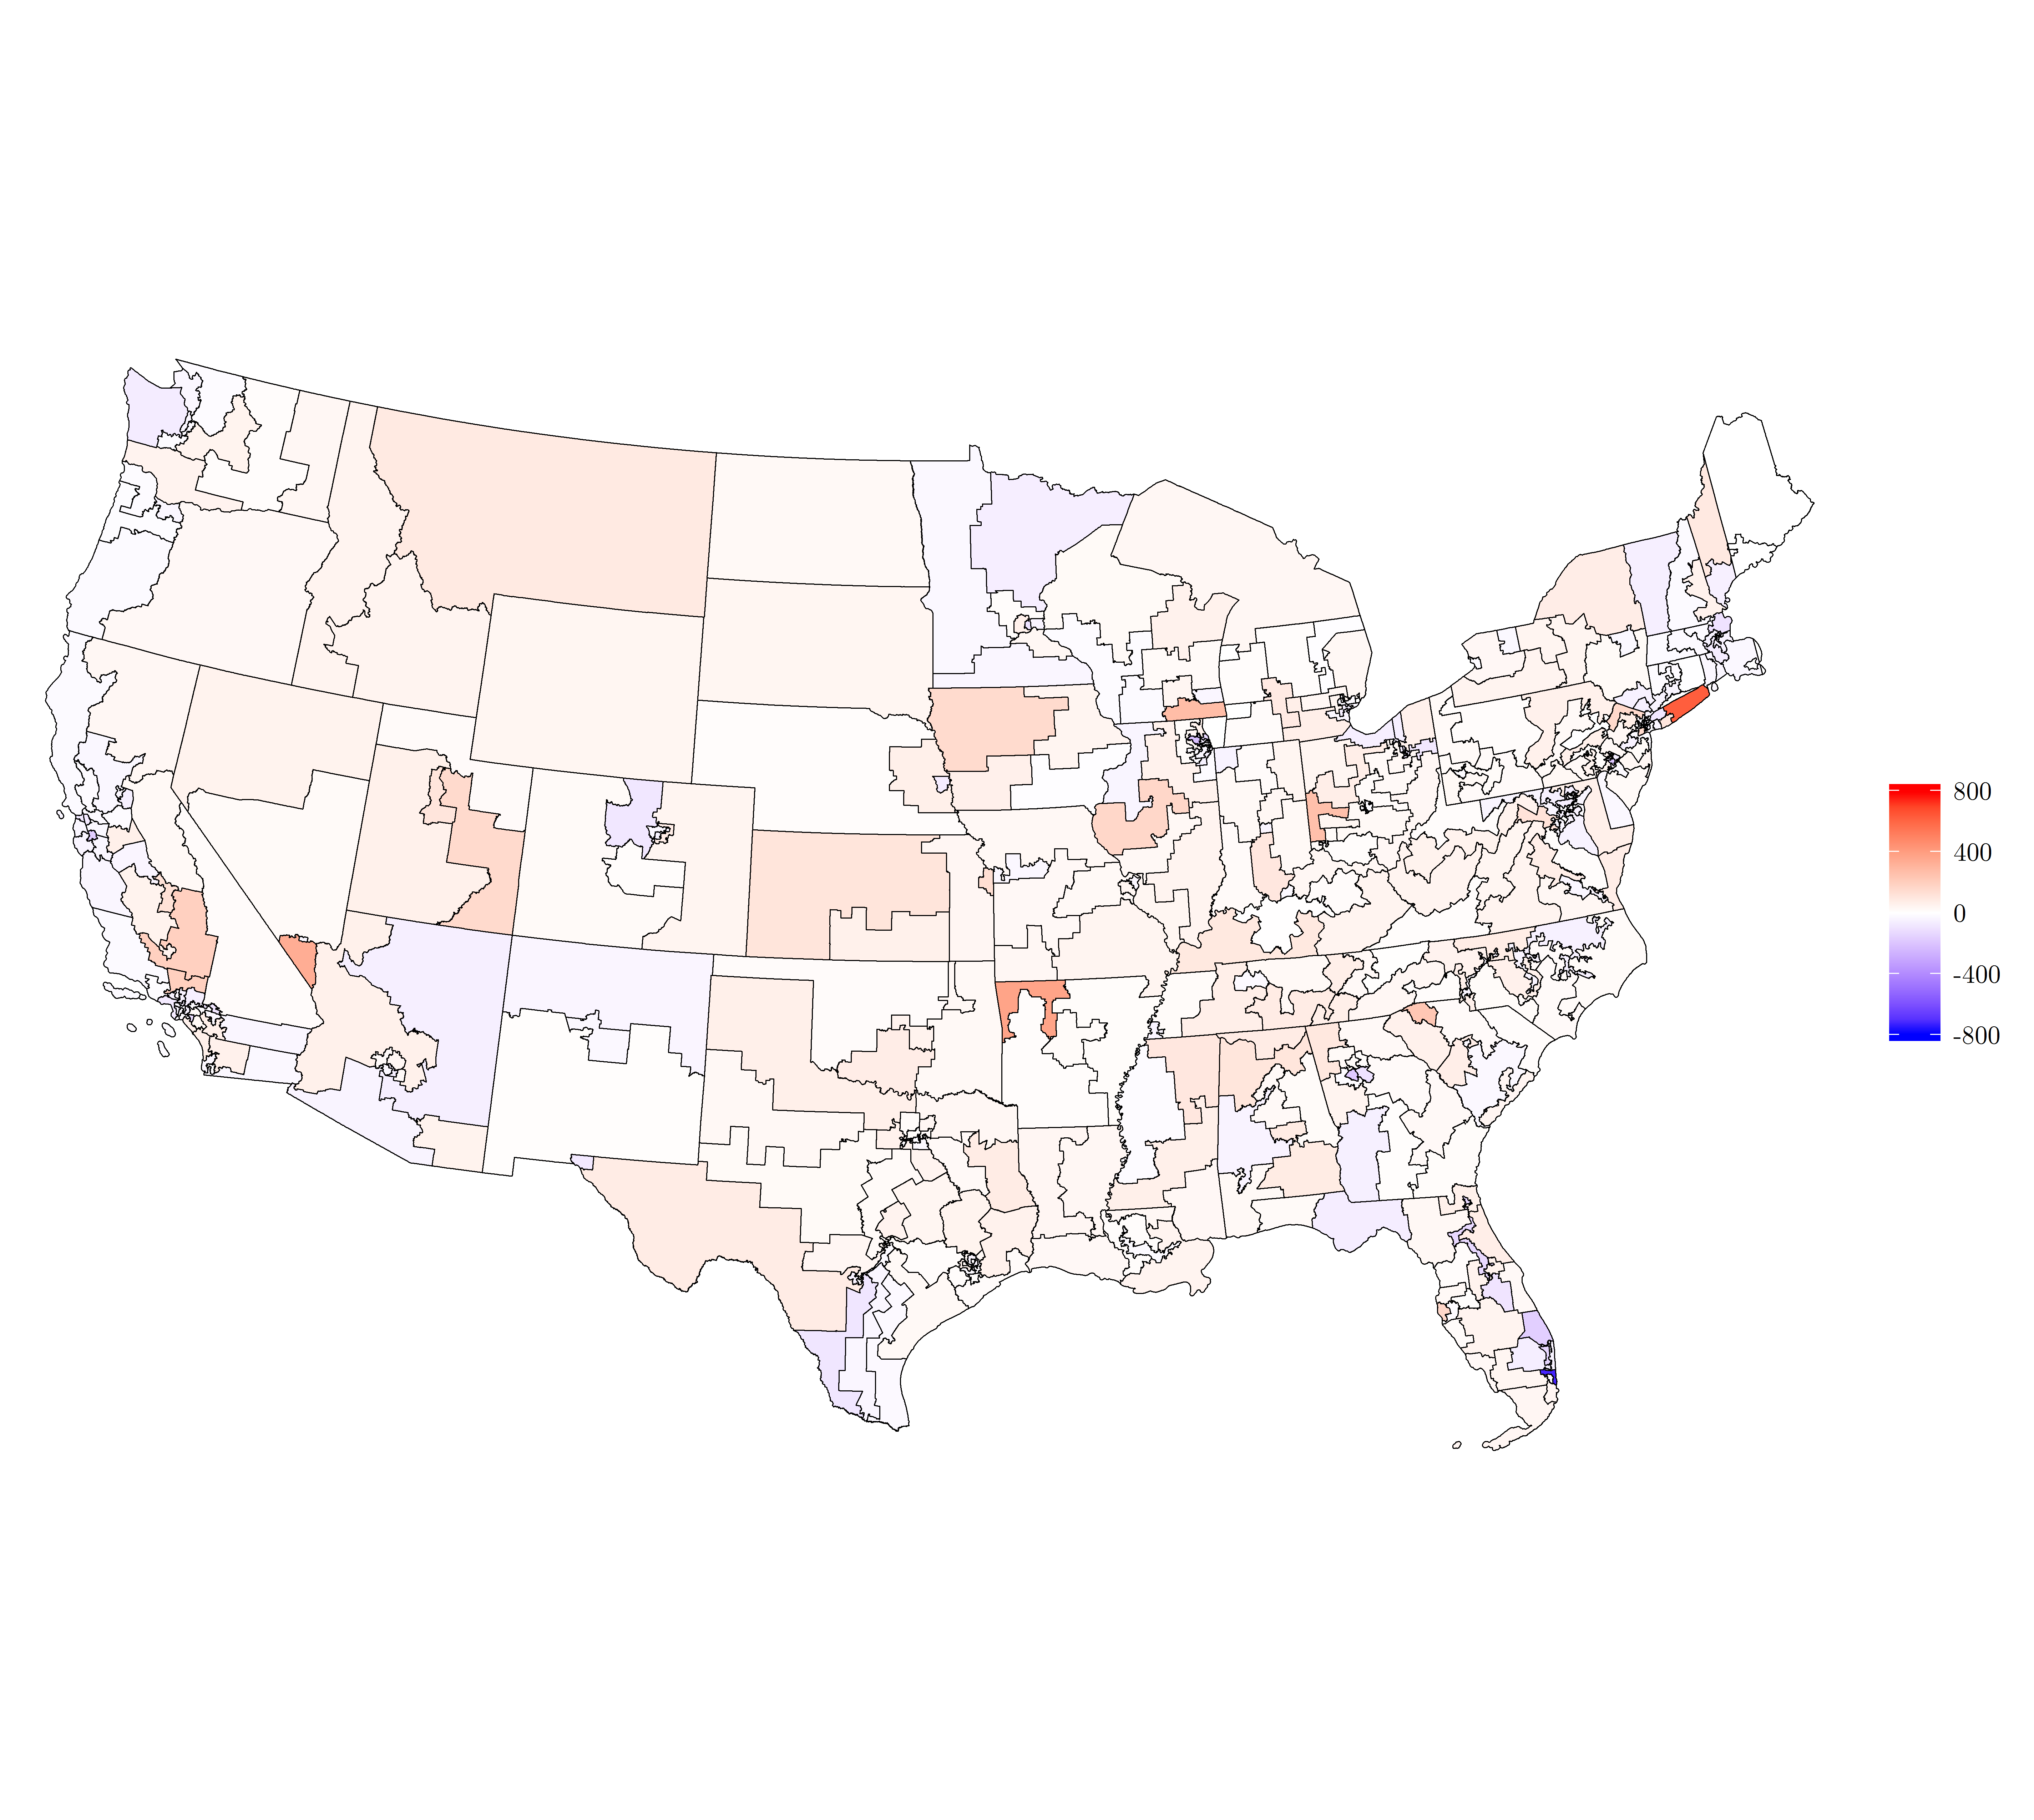
\includegraphics[scale=.17]{uc_5_map_editsbefore.png}
	\vspace{0cm} \\
\hspace*{-0.8cm}
	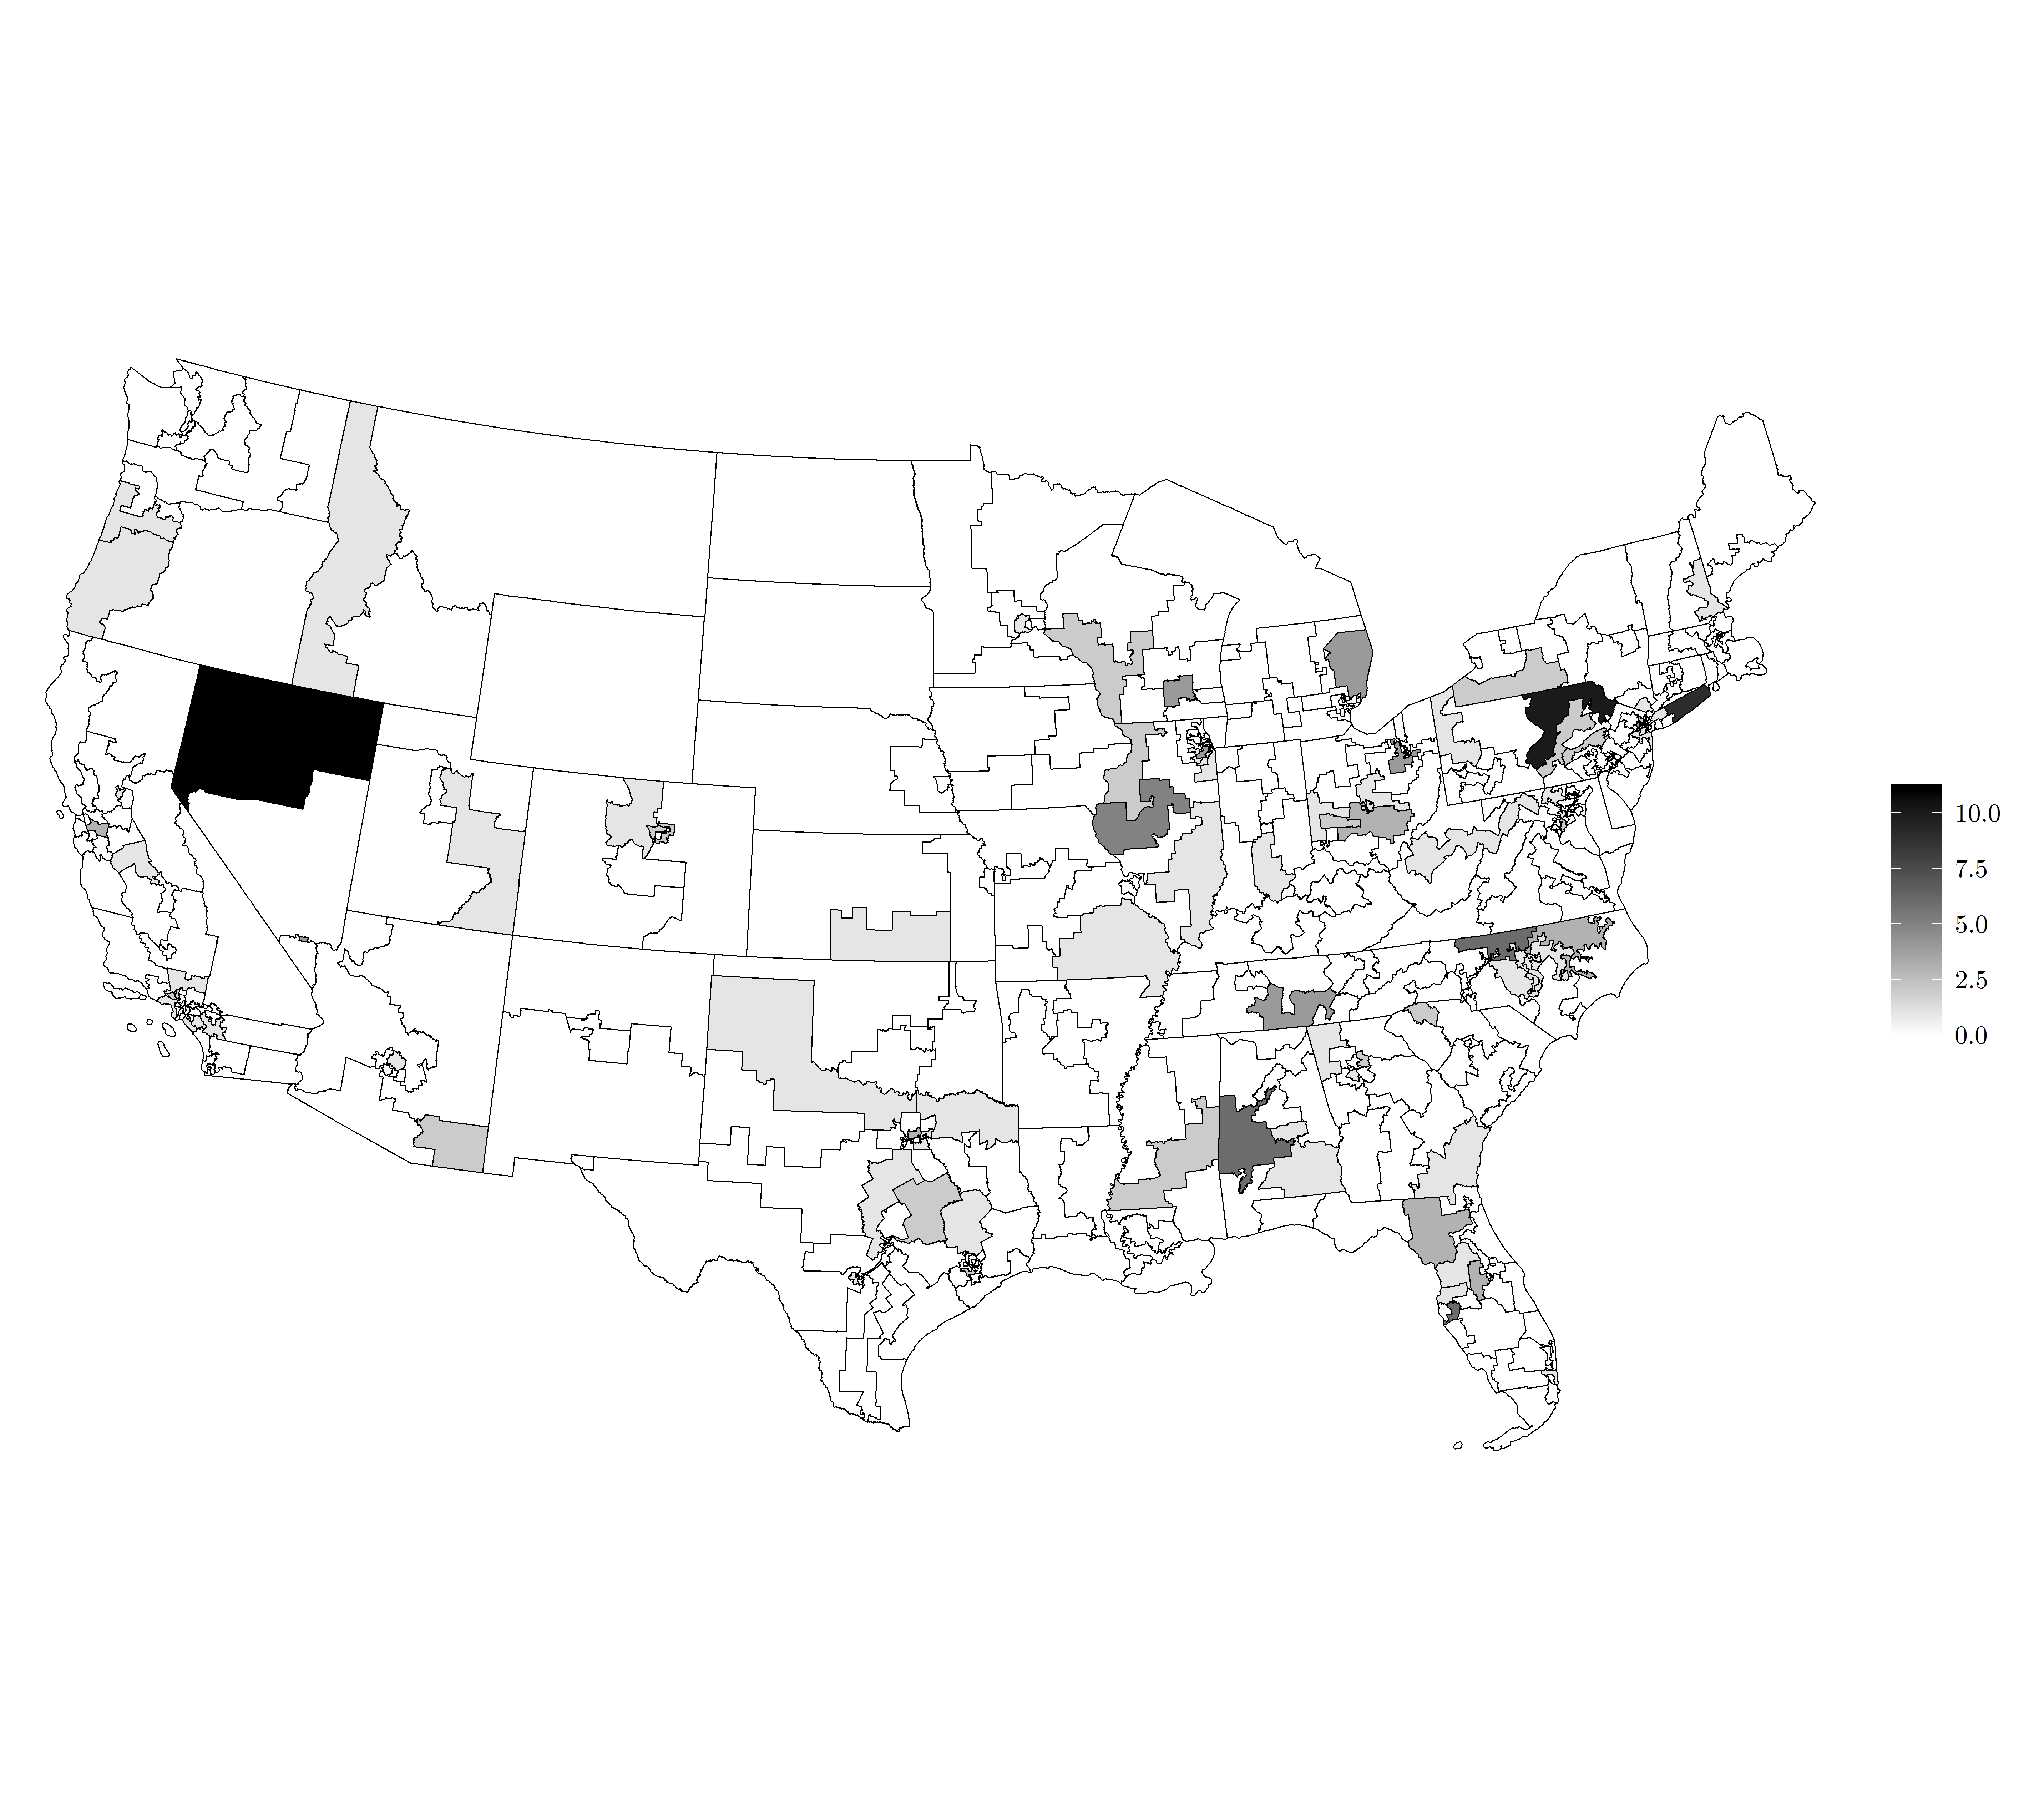
\includegraphics[scale=.17]{uc_5_map_editsanon1.png}
\hspace*{-0.1cm}
	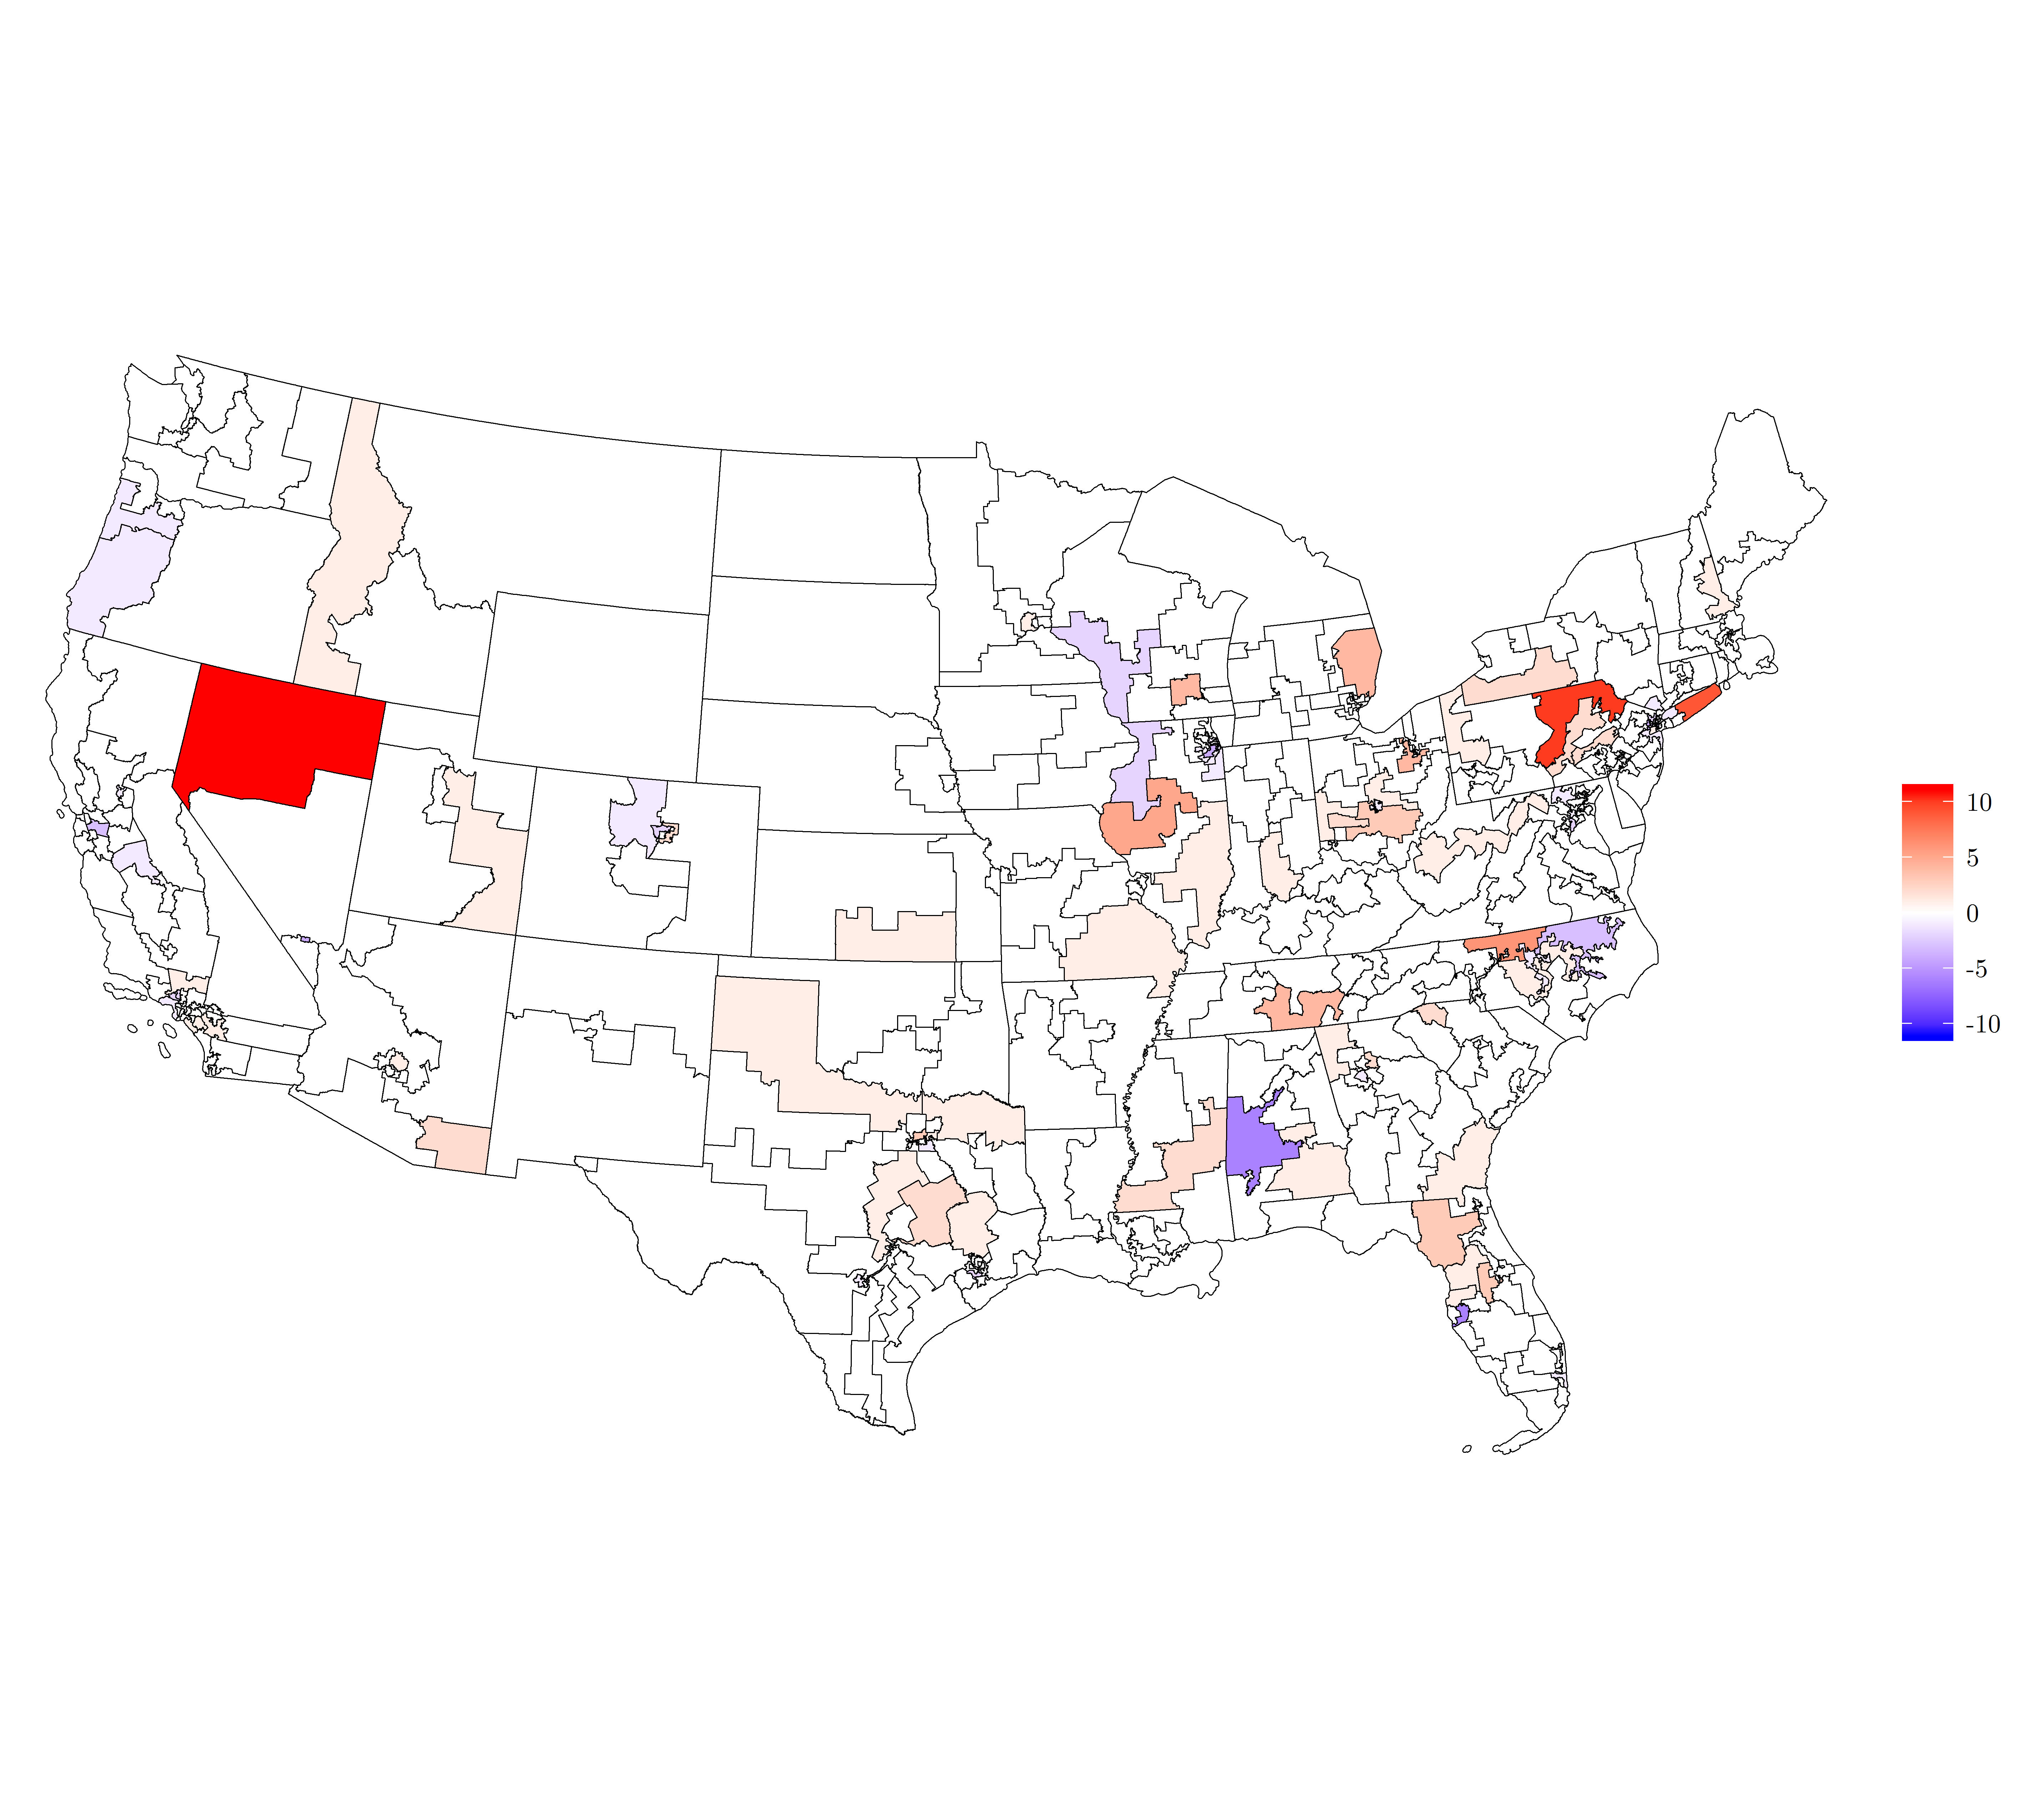
\includegraphics[scale=.17]{uc_5_map_editsanon2.png}
\hspace*{-0.1cm}
	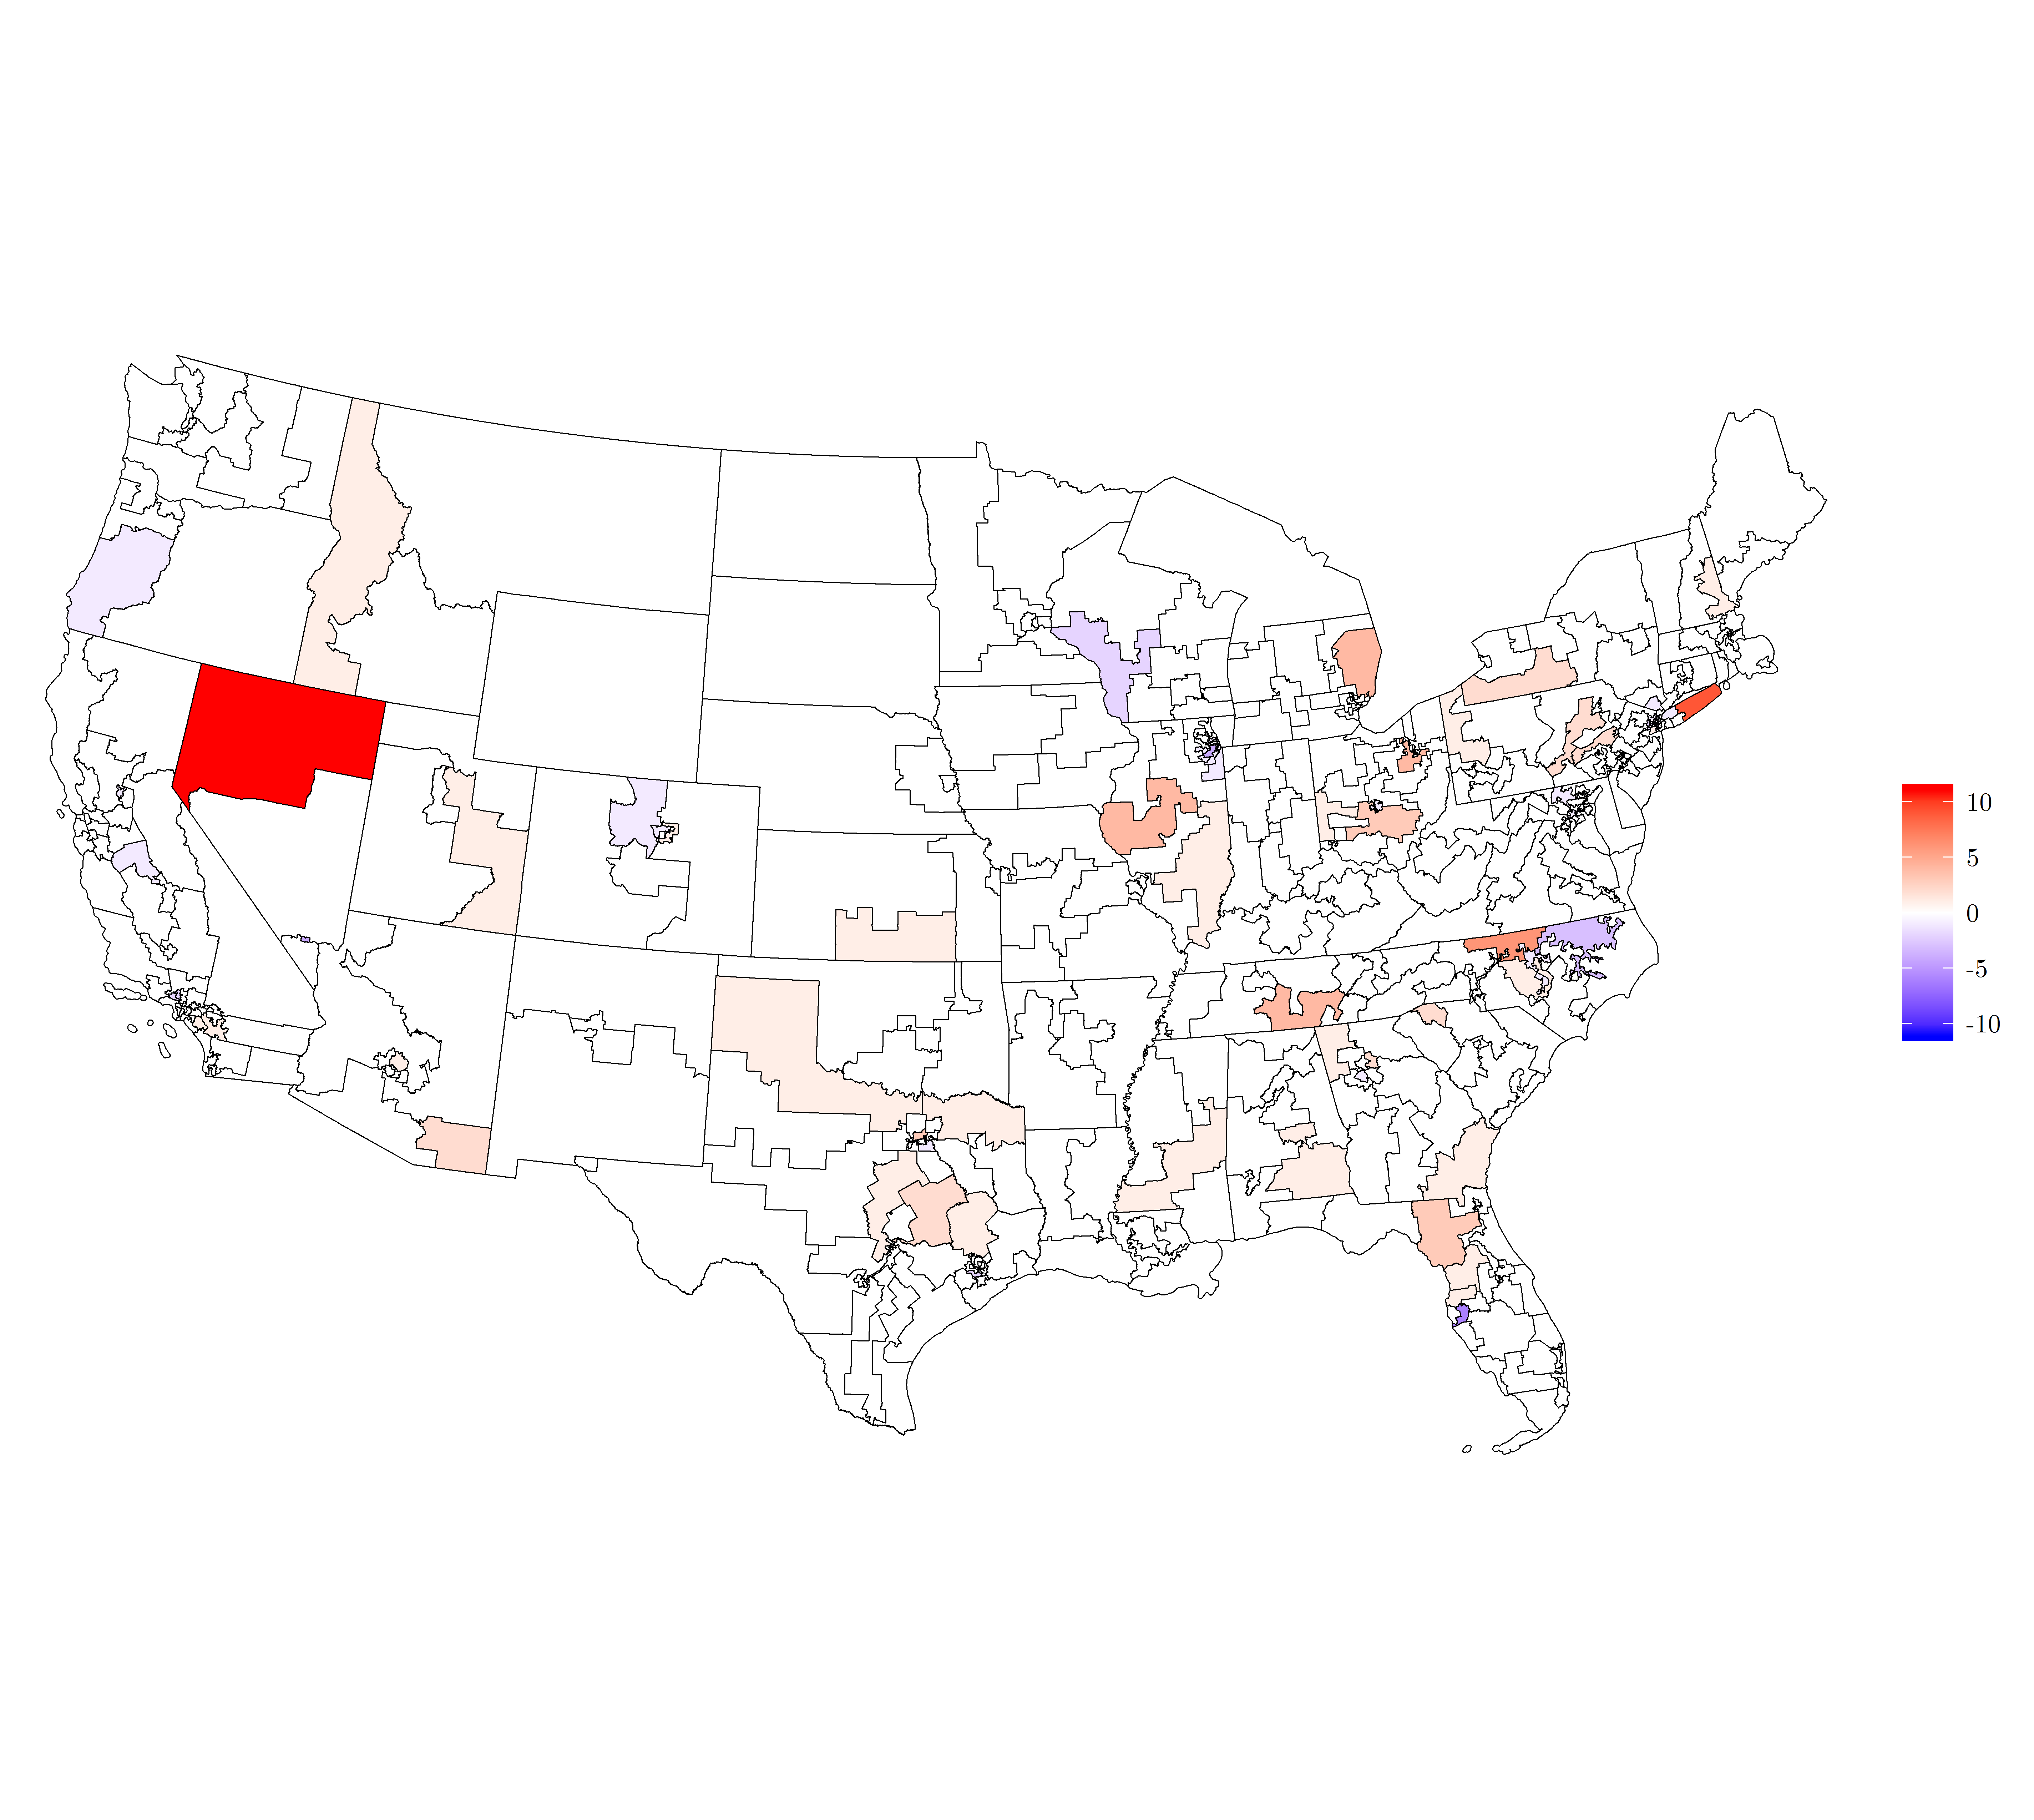
\includegraphics[scale=.17]{uc_5_map_editsanonbefore.png}
\end{center}
\end{figure}
\begin{tikzpicture}[remember picture,overlay]
\node at (5.3,7.75) {\small all edits};
\node at (5.3,4) {\small ISP -- House};
\end{tikzpicture}
\end{frame}

\begin{frame}{Use Cases (6)}
\begin{figure}[t]
\begin{center}
\vspace{-.3cm}
\hspace*{-0.5cm}
	
\includegraphics[scale=.33]{uc_5_wc_dels.png}
\hspace*{0.4cm}
	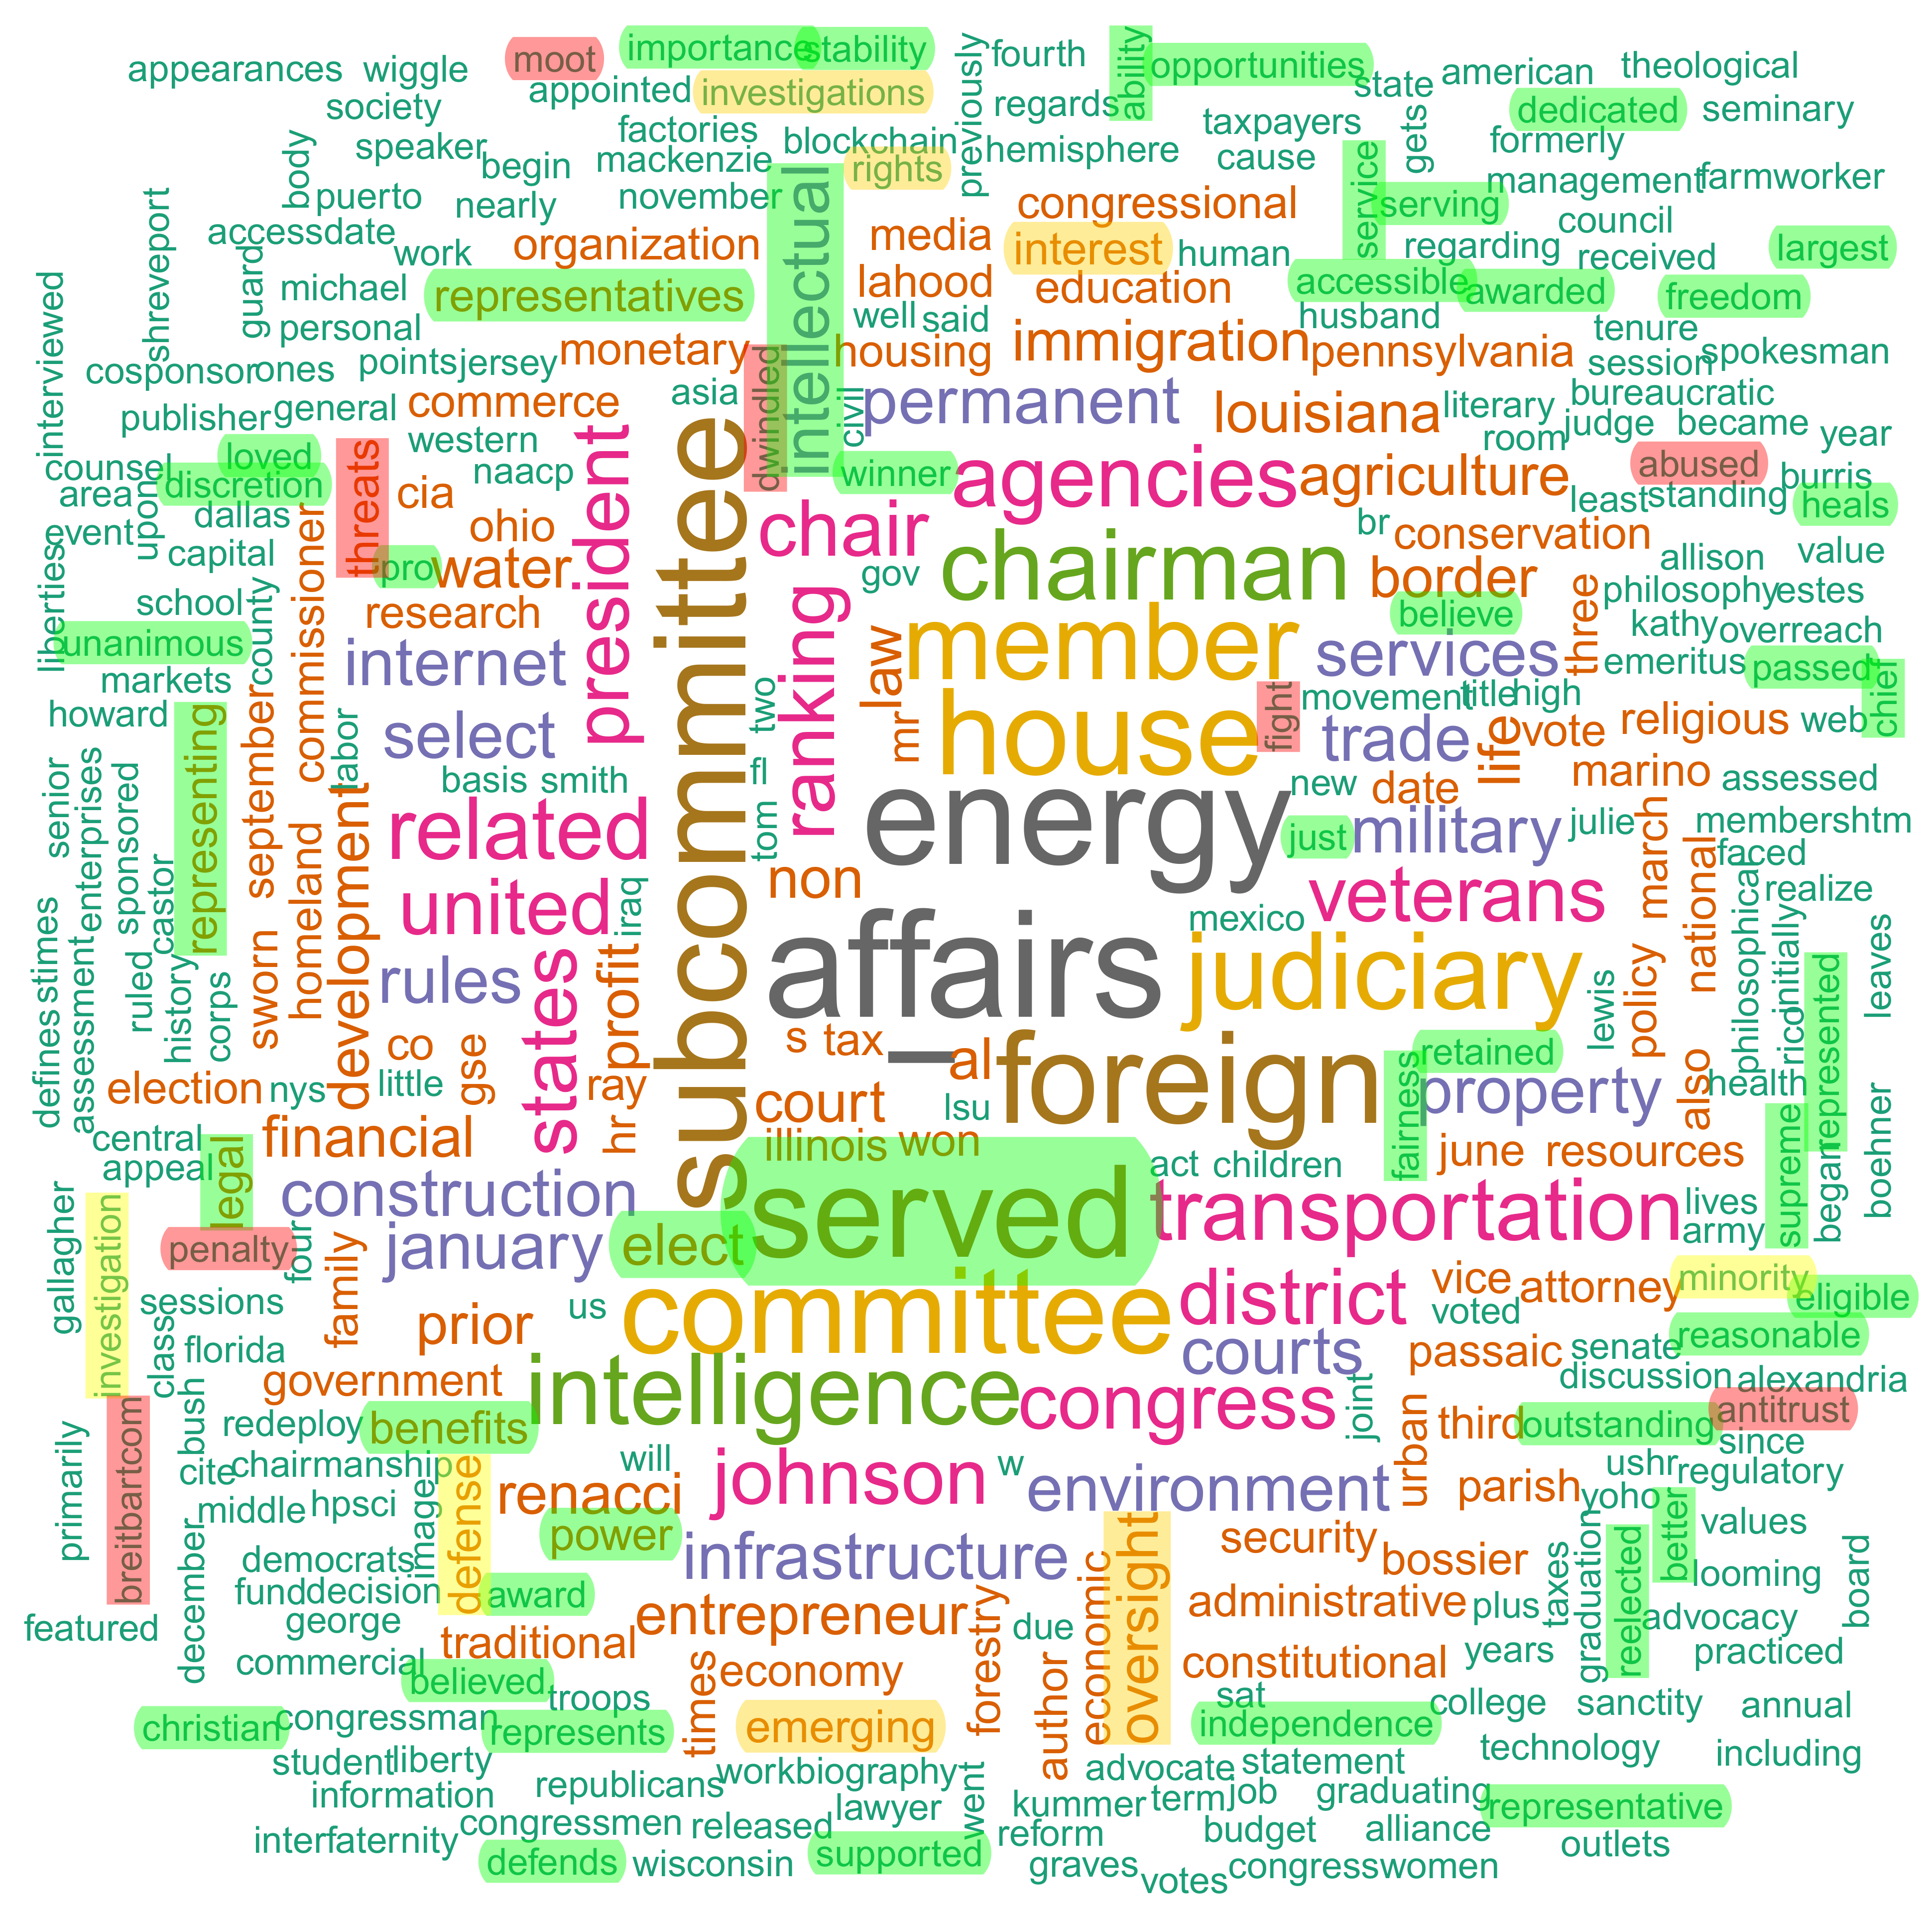
\includegraphics[scale=.33]{uc_5_wc_ins.png}
	\vspace{-.5cm}
\end{center}
\end{figure}
\begin{tikzpicture}[remember picture,overlay]
\node at (5.3,0) {\small sentiment};
\node at (2.3,0) {\small -0.4};
\node at (8.3,0) {\small +1.3};
\node at (2.3,6.5) {\small deletions};
\node at (8.3,6.5) {\small insertions};
\end{tikzpicture}
\end{frame}
\fi

\iffalse
\begin{frame}
\vspace{2.5cm}
\begin{center}
\LARGE Thank you for your attention!
\end{center}
\vspace{1.5cm}
\begin{flushright}
Sascha Göbel \\
\url{sascha.goebel@uni-konstanz.de} \\ 
\smallskip
Simon Munzert \\
\url{munzert@hertie-school.org} \\
\end{flushright}
\end{frame}
\fi

\end{document}
